
%%%%%%%% ICML 2018 EXAMPLE LATEX SUBMISSION FILE %%%%%%%%%%%%%%%%%

\documentclass{article}
\usepackage[margin=1in]{geometry}
\usepackage{dblfloatfix}    % To enable figures at the bottom of page
% Recommended, but optional, packages for figures and better typesetting:
\usepackage{microtype}
\usepackage{graphicx}
%\usepackage{subfigure}
\usepackage{booktabs} \usepackage{stmaryrd}% for professional tables
 
\usepackage[section]{placeins}
% hyperref makes hyperlinks in the resulting PDF.
% If your build breaks (sometimes temporarily if a hyperlink spans a page)
% please comment out the following usepackage line and replace
% \usepackage{icml2018} with \usepackage[nohyperref]{icml2018} above.
%\usepackage{hyperref}

% Attempt to make hyperref and algorithmic work together better:
\newcommand{\theHalgorithm}{\arabic{algorithm}}

\newcommand{\system}{\textsc{DreamCoder}~}
\newcommand{\systemEnding}{\textsc{DreamCoder}}
\newcommand{\lowerBound}{\mathscr{L}}
\newcommand{\denotation}[1]{{\llbracket #1 \rrbracket}}
\newcommand{\code}[1]{{\footnotesize\texttt{#1}}}
\newcommand{\scode}[1]{{\tiny\texttt{#1}}}
\newcommand{\mcode}[1]{{\scriptsize\texttt{#1}}}
\newcommand{\codechar}[1]{{\footnotesize{\texttt{"#1"}}}}
% Use the following line for the initial blind version submitted for review:
%\usepackage[nohyperref]{icml2018}

\usepackage{xcolor}
\definecolor{pop1}{HTML}{1F78b4}
\definecolor{pop2}{HTML}{164C13}
\definecolor{pop3}{HTML}{d95F02}
\definecolor{orange}{HTML}{d95F02}
\definecolor{teal}{HTML}{1b9e77}
\newcommand{\pop}[1]{\textcolor{pop1}{#1}}
\newcommand{\popp}[1]{\textcolor{pop2}{#1}}
\newcommand{\tree}[1]{\textcolor{pop3}{#1}}
\newcommand{\orange}[1]{\textcolor{orange}{#1}}
\newcommand{\teal}[1]{\textcolor{teal}{#1}}

\newcommand{\greenCode}[1]{{\footnotesize\popp{\code{#1}}}}
\newcommand{\blueCode}[1]{{\footnotesize\pop{\code{#1}}}}

%\usepackage{hyperref}       % hyperlinks
\usepackage{url}            % simple URL typesetting
\usepackage{booktabs}       % professional-quality tables
\usepackage{amsfonts}       % blackboard math symbols
\usepackage{nicefrac}       % compact symbols for 1/2, etc.
\usepackage{microtype}      % microtypography
\usepackage{mathrsfs}
\usepackage{listings}
\usepackage{amsthm}
% use Times
\usepackage{times}
% For figures
\usepackage{graphicx} % more modern
%\usepackage{epsfig} % less modern
\usepackage{subfig} 
\usepackage{fancyvrb}


\usepackage{caption}
%\usepackage{subcaption}

\fvset{fontsize=\footnotesize}

\usepackage{amssymb}
\usepackage{listings}
\usepackage{wrapfig}
\usepackage{tabularx}


\usepackage{verbatim}
 \usepackage{booktabs}
 % For algorithms
\usepackage{algorithm}
%\usepackage{algorithmic}
\usepackage{algpseudocode}% http://ctan.org/pkg/algorithmicx
\usepackage{tikz}
\usepackage{circuitikz}
\usetikzlibrary{fit,bayesnet,calc,tikzmark}
\usetikzlibrary{arrows.meta}
\usetikzlibrary{positioning}
\usetikzlibrary{decorations.text}
\usetikzlibrary{decorations.pathmorphing}
\tikzset{squiggle/.style={decorate, decoration={snake,amplitude=.4mm}}}
\usepackage{dsfont}
\usepackage{amsmath}

\DeclareMathOperator*{\argmin}{arg\,min} % thin space, limits underneath in displays
\DeclareMathOperator*{\argmax}{arg\,max} % thin space, limits underneath in displays
 


% Packages hyperref and algorithmic misbehave sometimes.  We can fix
% this with the following command.

\newcommand{\Expect}{\mathds{E}} %{{\rm I\kern-.3em E}}
\newcommand{\indicator}{\mathds{1}} %{{\rm I\kern-.3em E}}
\newcommand{\expect}{\mathds{E}} %{{\rm I\kern-.3em E}}
\newcommand{\probability}{\mathds{P}} %{{\rm I\kern-.3em P}}
\newcommand{\shift}[1]{\uparrow^{#1}}
\newcommand{\downshift}[1]{\downarrow^{#1}}
\newcommand{\substitute}[2]{[\$ #1 \mapsto #2]}
\newcommand{\reduce}{\longrightarrow}
\newcommand{\manyReduce}{\longrightarrow^*}

\newtheorem{definition}{Definition}
\newtheorem{theorem}{Theorem}
\newtheorem{lemma}{Lemma}

\newcommand{\NeuralNetwork}[1]{    \begin{tikzpicture}[x=2.5cm,y=1.25cm,transform canvas={scale=#1,shift={+(-1,2.5)}}]
      \tikzstyle{neuron}=[circle,fill=blue!50,minimum size=20pt]
      \fill[fill=white] (-0.25,-0.5) rectangle (2.25,-4.5);
      \node[rectangle] at (1,1) {};
      \foreach \name / \y in {1,...,4}
          \node[neuron] (I-\name) at (0,-\y) {};
      \foreach \name / \y in {1,...,3}
          \node[neuron] (H-\name) at (1,-\y-0.5) {};
      \foreach \name / \y in {1,...,4}
          \node[neuron] (O-\name) at (2,-\y) {};
      \foreach \source in {1,...,4}
          \foreach \dest in {1,...,3}
              \draw [-latex] (I-\source) -- (H-\dest);
      \foreach \source in {1,...,3}
          \foreach \dest in {1,...,4}
              \draw [-latex] (H-\source) -- (O-\dest);
    \end{tikzpicture}}
\newcommand{\spiral}[2]{
  \draw[ultra thick,->] ([shift={#1}]-30:#2) arc [radius = #2, start angle = -30, end angle = 90];
  \draw[ultra thick,->] ([shift={#1}]-30:#2) arc [radius = #2, start angle = -30, end angle = 95];

  
      \draw[ultra thick,->] ([shift={#1}]90:#2) arc [radius = #2, start angle = 90, end angle = 210];
      \draw[ultra thick,->] ([shift={#1}]90:#2) arc [radius = #2, start angle = 90, end angle = 205];
      
      \draw[ultra thick,->] ([shift={#1}]210:#2) arc [radius = #2, start angle = 210, end angle = 340];
      \draw[ultra thick,->] ([shift={#1}]210:#2) arc [radius = #2, start angle = 210, end angle = 335];
}
\newcommand{\legend}{
  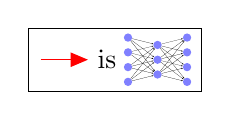
\begin{tikzpicture}
    \node at (0,0) (uses){is};
    \draw[->,red] ([xshift=-0.6cm]uses.west)  -- (uses.west);
    \node at ([xshift=0.4cm]uses.east) {\NeuralNetwork{0.15}};
    \draw[thin] (-1,-0.4) rectangle (1.2,0.4);
  \end{tikzpicture}
  }

\tikzstyle{vecArrow} = [thick, decoration={markings,mark=at position                                
   1 with {\arrow[semithick]{open triangle 60}}},                                                   
   double distance=1.4pt, shorten >= 5.5pt,                                                         
   preaction = {decorate},                                                                          
   postaction = {draw,line width=1.4pt, white,shorten >= 4.5pt}]                                    
\tikzstyle{innerWhite} = [semithick, white,line width=1.4pt, shorten >= 4.5pt]                      
         
\begin{document}

\begin{figure}
  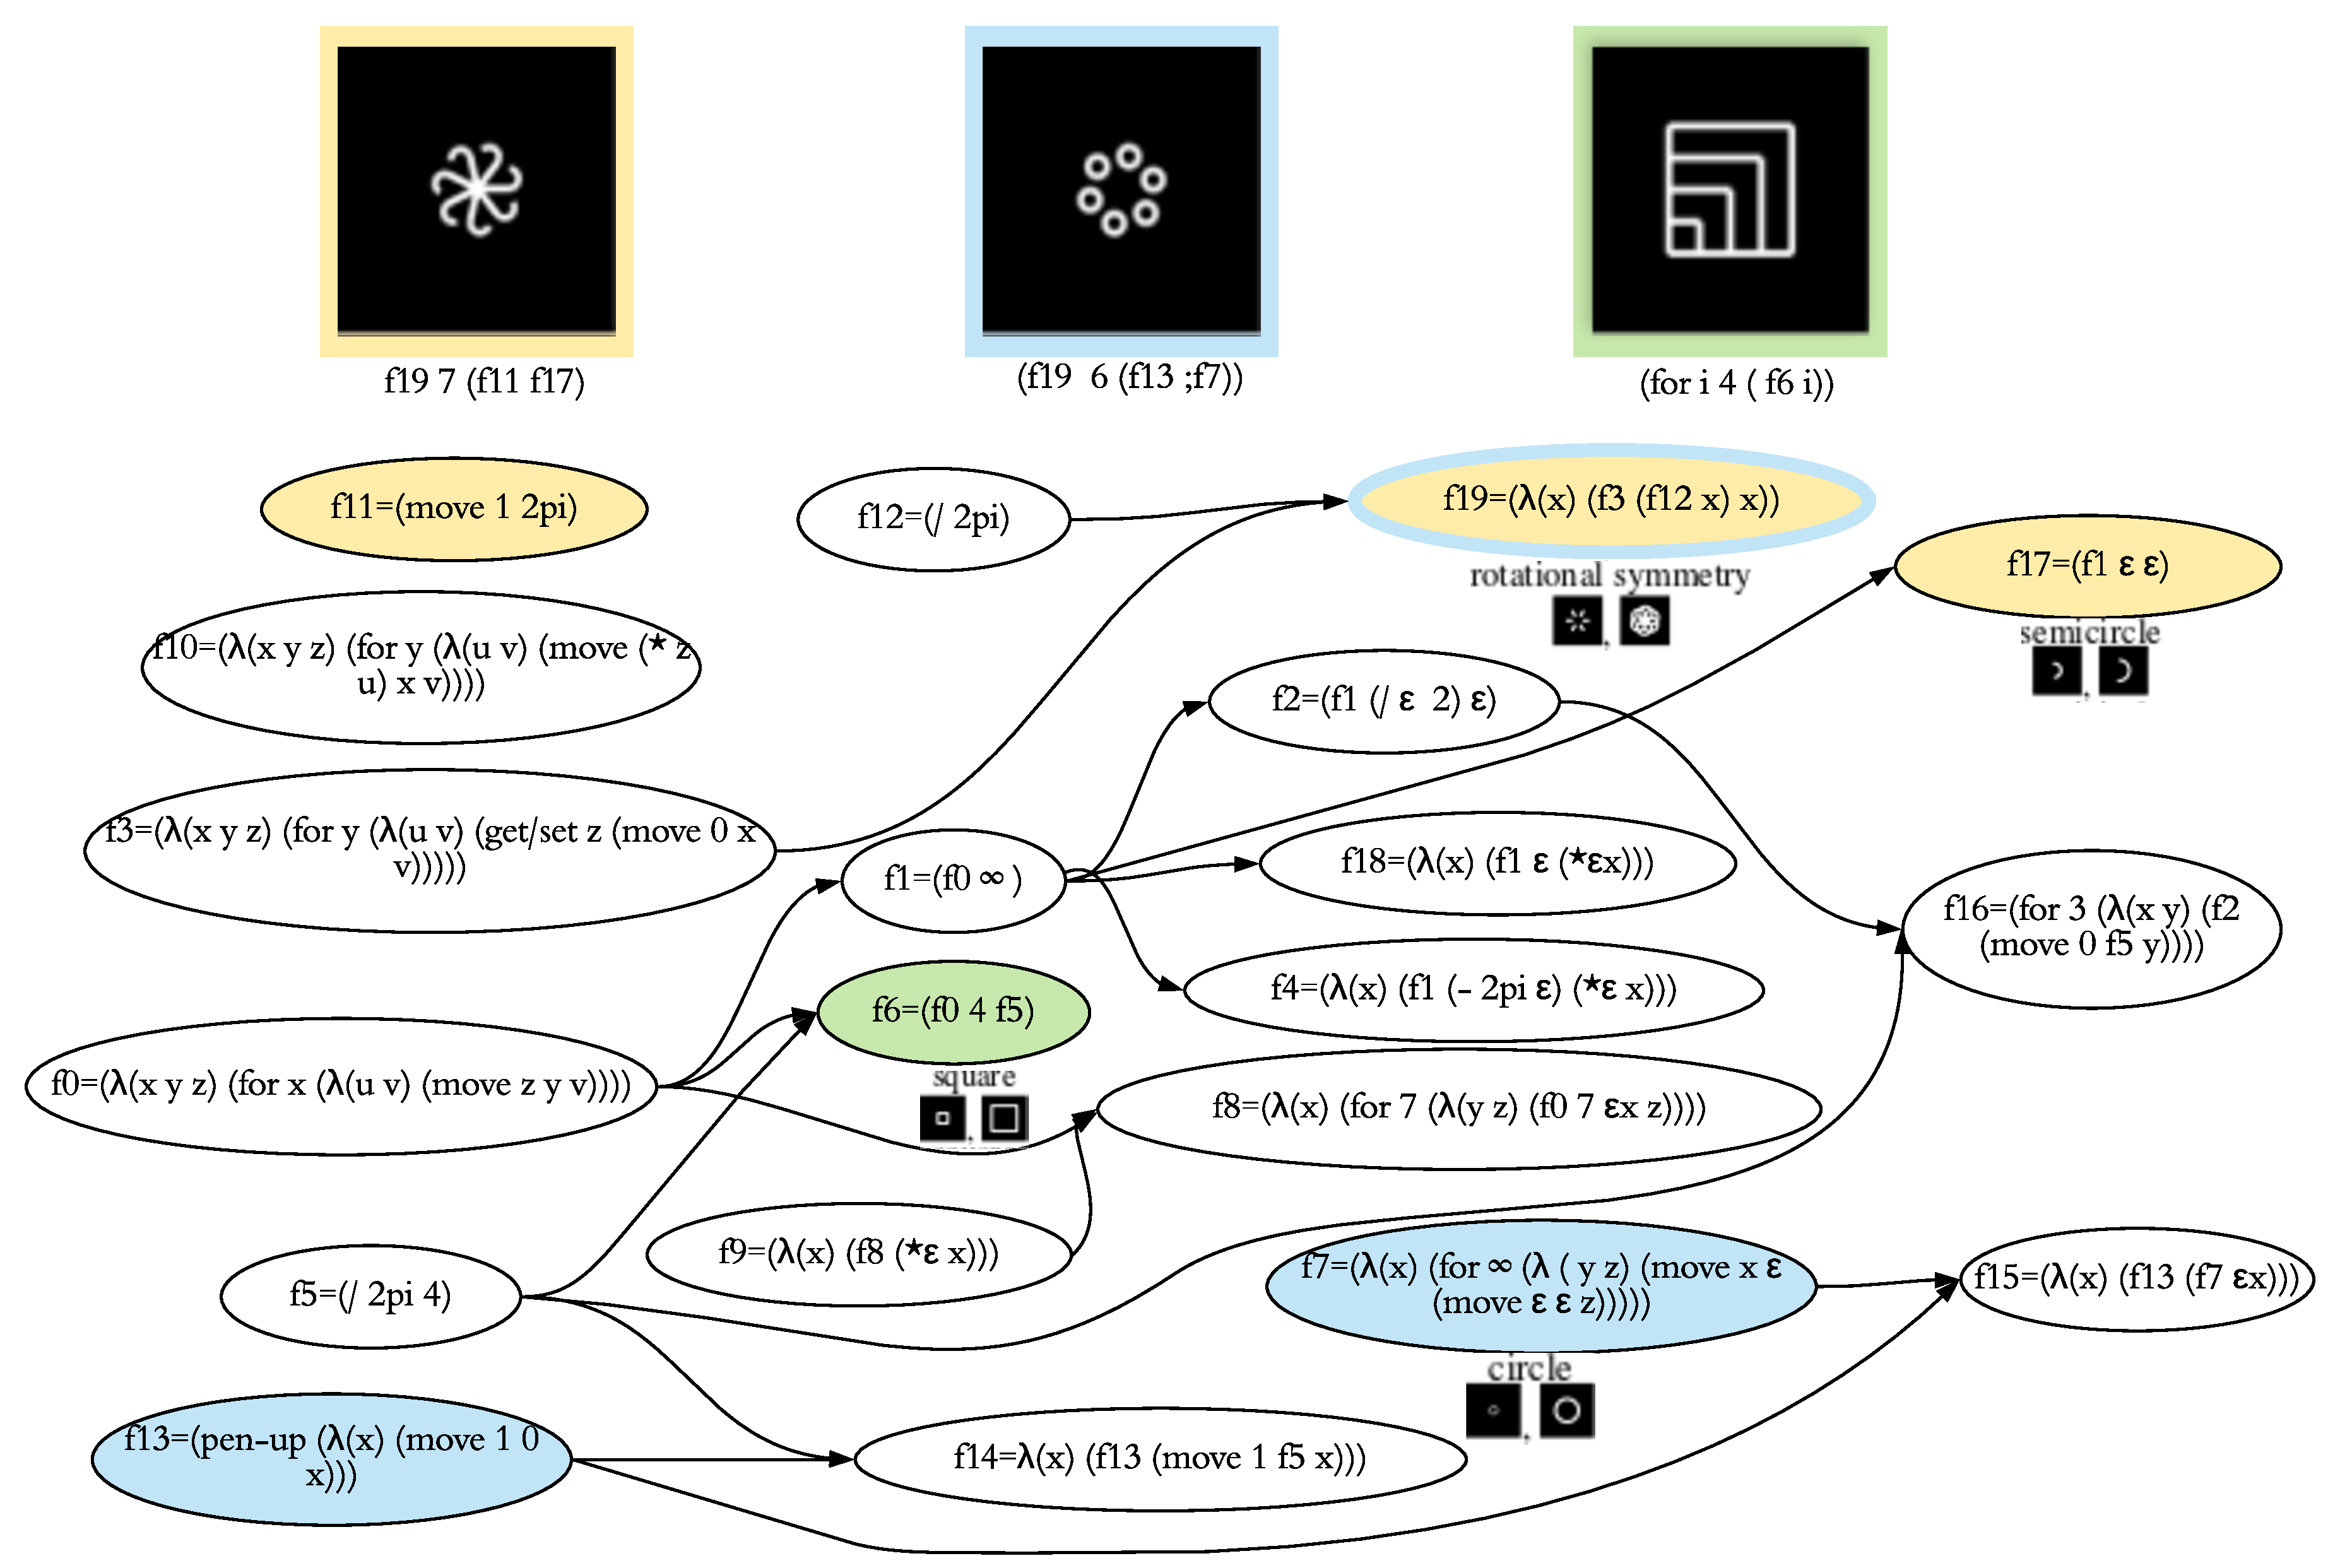
\includegraphics[width = \textwidth]{figures/DeepLogo.pdf}
  \caption{\textbf{Bottom}: Learned graphics programing DSL. Each circle encloses a different learned component; arrows point from a component to other components that use it. \textbf{Top}: 3 tasks, and below them the programs that solve them. Yellow/Blue/Green highlighting indicates which DSL components are used to solve which tasks.}
  \end{figure}

\begin{figure}
  \begin{tikzpicture}
    \renewcommand{\baselinestretch}{0.5}
    \renewcommand{\inventionColor}{orange}
    \newcommand{\name}[2]{
      \mcode{{\color{\inventionColor}$f_{#1}$}$($#2$)\,=\,$}
    }
    \newcommand{\noArguments}[1]{
      \mcode{{\color{\inventionColor}$f_{#1}\,=\,$}}
    }

    
    \renewcommand{\horizontalSpacing}{3.8cm}
    \renewcommand{\verticalSpacing}{2cm}

    
%    \draw (0,0) rectangle (10,5);
    \node(t1)[align=left] at (1,-1) {
      \footnotesize +106 769-43$\to $106.769.43\\
      \footnotesize +83 973-831$\to $83.973.831\\
      \footnotesize $f(\text{\mcode{s}}) = $\mcode{(}\subnode{f01}{${\color{\inventionColor}f_0}$}\mcode{  \codechar{.} \codechar{-}}\\
      \footnotesize \hspace{1.25cm}\mcode{(${\color{\inventionColor}f_0}$ \codechar{.} \codechar{ }}\\
      \footnotesize \hspace{1.4cm}\mcode{(cdr s)))}
    };
    \node(t2)[align=left,anchor=center] at ([xshift=\horizontalSpacing]t1.center) {
      \footnotesize Dream Coder$\to$Dr. Dream\\
      \footnotesize Andy Cencici$\to$Dr. Andy\\
      \footnotesize Jan Kotas$\to$Dr. Jan\\
      \footnotesize Nancy Jones$\to$Dr. Nancy\\
      \footnotesize $f(\text{\mcode{s}}) = $\mcode{(${\color{\inventionColor}f_3}$ (${\color{\inventionColor}f_4}$ \codechar{ } s))}
    };
    \node(t3)[align=left] at ([xshift=2cm]t2.east) {
      \footnotesize Dream (Coder)$\to$Coder\\
      \footnotesize 1 (2) 3 4$\to$2\\
      \footnotesize the (dog) ran$\to$ran\\
      \footnotesize +817(33)99$\to$33\\
      \footnotesize $f(\text{\mcode{s}}) = $\mcode{(${\color{\inventionColor}f_6}$ \codechar{(} \codechar{)} s)}
    };

    \draw (-2,-2.5) -- (15,-2.5);
    \node[align=left,rotate=90] at (-1.5,-1.3) {Tasks and\\\\\texttt{Programs}};

    \node[align=left,rotate=90] at (-1.5,-6.3) {Domain Specific Language (DSL)\\\\System discovers subroutines in {\color{\inventionColor}orange}};

    
    \newcommand{\invention}[4]{
      \node(#1)[inner sep=1,anchor=center,text width=2cm,draw,rounded corners,align=center] at (#2) {
        \footnotesize #3
      };
      \node[anchor=north] at ([yshift=3.5pt]#1.south) {#4};
    }
    \newcommand{\vinvention}[4]{
      \invention{#1}{[yshift=-\verticalSpacing]#2.center}{#3}{#4}
    }
    \newcommand{\hinvention}[4]{
      \invention{#1}{[xshift=\horizontalSpacing]#2.center}{#3}{#4}
    }


    \invention{substitution}{1,-4}{
      ${\color{\inventionColor}f_0}($\mcode{s}$,$\mcode{a}$,$\mcode{b}$) \,=\, $\\
       \mcode{(map ($\lambda$ (x) (if (= x a)\\ b x)) s)}
    }{substitute chars}
    \vinvention{cat}{substitution}{
      ${\color{\inventionColor}f_1}($\mcode{a}$,$\mcode{b}$) \,=\, $\\
      \mcode{(fold ($\lambda$ (x y)\\ (cons x y))\\ a b))}
    }{concat strings}
    \vinvention{looping}{cat}{
       ${\color{\inventionColor}f_2}($\mcode{c}$,$\mcode{p}$,$\mcode{s}$) \,=\, $\\
      \mcode{(unfold l ($\lambda$ (x) (= c (car x))) p ($\lambda$ (z) (cdr z)))}
    }{loop until char}

    \hinvention{constant}{substitution}{
      ${\color{\inventionColor}f_3}($\mcode{s}$) \,=\, $\\
      \mcode{(${\color{\inventionColor}f_1}$ s string)}
    }{prepend constant}
    \vinvention{drop}{constant}{
      ${\color{\inventionColor}f_4}($\mcode{c}$) \,=\, $\\
      \mcode{(${\color{\inventionColor}f_2}$ c ($\lambda$ }\\\mcode{(z) (car z)))}
    }{prefix}
    \vinvention{suffix}{drop}{
      ${\color{\inventionColor}f_5}($\mcode{s}$,$\mcode{c}$) \,=\, $\\
      \mcode{(fold ($\lambda$ (x y) }\\\mcode{(cdr (if (= x c)}\\\mcode{ s y))) s s)}
    }{suffix}

    \hinvention{delimited}{constant}{
      \mcode{${\color{\inventionColor}f_6}($x$,$y$,$s$)\,=\,$}\\
      \mcode{(${\color{\inventionColor}f_4}$ x (${\color{\inventionColor}f_5}$ y c))}
    }{delimited substring}
    \draw[->] (delimited.west) -- (drop.east);
    \draw[->] (delimited.west) -- (suffix.east);

    \vinvention{appendSingle}{delimited}{
      \mcode{${\color{\inventionColor}f_7}($c$,$s$)\,=\,$}\\
      \mcode{(${\color{\inventionColor}f_1}$ (cons c nil) s)}}{append character}
    
    \vinvention{surround}{appendSingle}{
      \mcode{${\color{\inventionColor}f_8}($s$)\,=\,$}\\
      \mcode{(cons \codechar{(} (${\color{\inventionColor}f_7}$ \codechar{)} s))}}{surround in parens}
    \draw[->] (surround.west) to[in=200,out=160] ([yshift=-0.25cm]appendSingle.west);
    \draw[->] (appendSingle.west) to[in=40,out=120] ([yshift=0.25cm]cat.east);
    
    \draw[->] (drop.west) -- (looping.east);
    \draw[->] (constant.west) -- (cat.east);

    \draw[->] ([xshift=-0.5cm]t2.south) -- (constant.north);
    \draw[->] ([xshift=0.3cm]t2.south) to[in=30,out=-30] ([xshift=1cm]drop.north);

    \draw[->] ([yshift=0.2cm,xshift=-0.2cm]t1.south) to[in=100,out=200] (substitution.north);
    \draw[->] ([yshift=0.5cm,xshift=-0.5cm]t1.south) to[in=120,out=200] ([xshift=-0.5cm]substitution.north);
    \draw[->] ([xshift=-0.5cm]t3.south) -- (delimited.north);
          
    \begin{scope}[shift={(0,-15)}]
      \invention{filter}{0,0}{
        \name{0}{p$,$z}\mcode{\\(fold ($\lambda$ (x a)\\ (if (p x) (cons x a) a))\\ nil z)} 
        }{higher-order `filter'}

      \vinvention{three}{filter}{\footnotesize ${\color{\inventionColor}f_1} = $\\\mcode{(+ 1 (+ 1 1))}}{The number `3'}
      \vinvention{prefix}{three}{\name{2}{n$,$z}\\\mcode{(map ($\lambda$ (i) (index i z)) (range (+ 1 n)))}}{First $n$ elements}
      \hinvention{single}{filter}{\name{3}{z$,$l}\\\mcode{(fold ($\lambda$ (x y)\\(cons x y))\\ z l)}}{Append element}
      \vinvention{for}{single}{\footnotesize ${\color{\inventionColor}f_4} = $\mcode{(+ 1 ${\color{\inventionColor}f_1}$)}}{The number `4'}
      \vinvention{Max}{for}{\name{5}{l}\\\mcode{%
          (car (${\color{\inventionColor}f_0}$ ($\lambda$ (x) (nil? (${\color{\inventionColor}f_0}$ l ($\lambda$ (z) (> z x))))) l))}}{max of list}
      \hinvention{largest}{single}{\name{6}{l$,$n}\\\mcode{(${\color{\inventionColor}f_5}$ (${\color{\inventionColor}f_0}$ ($\lambda$ (x) \\(> n (length (${\color{\inventionColor}f_0}$ ($\lambda$ (y) (> x y)) l)))) l))}}{$n^{\text{th}}$ largest element}
      \vinvention{count}{largest}{\name{7}{p$,$l}\\\mcode{(length\\ (${\color{\inventionColor}f_0}$ ($\lambda$ (y) (= x y)) l))}}{count}
      \vinvention{weird}{count}{\name{8}{p$,$l}\mcode{
          (map ($\lambda$ (x) (if (p x) (+ 1 x) 0))))}}
                 {Higher-order incrementer}

      \draw[->] (for.west) -- (three.east);
      \draw[->] ([yshift=-0.0cm]largest.west) -- (Max.east);
      \draw[->] ([yshift=-0.cm]largest.west) to[out=240,in=330] ([yshift=-0.1cm]filter.east);
      \draw[->] (Max.west) -- (filter.east);
      \draw[->] ([yshift=0.1cm]count.west) -- ([yshift=-0.3cm]filter.east);

      \node(t1)[align=left,anchor=center] at (0,3) {
        \mcode{[1 4 5 8]$\to$[5 8]}\\
        \mcode{[9 8 3 8]$\to$[9 8 8]}\\
        \mcode{[3 4 5 6]$\to$[5 6]}\\
        \mcode{[6 5 4 3]$\to$[6 5]}\\
        \footnotesize $f(\text{\mcode{z}}) = $\mcode{(${\color{\inventionColor}f_0}$ ($\lambda$ (x)}\\\hspace{0.5cm}\mcode{ (> x ${\color{\inventionColor}f_4}$)) z)}
      };
      \node(t2)[align=left] at ([xshift=\horizontalSpacing]t1.center) {
        \mcode{[9 2 4]$\to$[4 2 9]}\\
        \mcode{[4 3]$\to$[3 4]}\\
        \mcode{[3 4 5 6]$\to$[6 5 4 3]}\\
        \mcode{[]$\to$[]}\\
        \footnotesize $f(\text{\mcode{z}}) = $\mcode{(fold ($\lambda$ (x a)}\\\hspace{0.25cm}\mcode{ (${\color{\inventionColor}f_3}$ x a)) nil z)}
      };
      \node(t3)[align=left] at ([xshift=\horizontalSpacing]t2.center) {
        \mcode{[9 2 3]$\to$[2 3 9]}\\
        \mcode{[2 1]$\to$[1 2]}\\
        \mcode{[8 7 9 2 5]$\to$[2 5 7 8 9]}\\
        \footnotesize $f(\text{\mcode{z}}) = $\mcode{(map ($\lambda$ (i)}\\\hspace{0.5cm}\mcode{(${\color{\inventionColor}f_6}$ z i)) }\\\hspace{0.5cm}\mcode{(+ 1 (range }\\\hspace{0.5cm}\mcode{(length z)))}
      };

      \draw[->] ([yshift=0.35cm,xshift=-0.3cm]t1.south) to[out=250] (filter.north);
      \draw[->] ([yshift=0.0cm,xshift=0.3cm]t1.south) to[out=350,in=100] (for.west);
      \draw[->] ([xshift=-0.7cm]t2.south) -- (single.north);
      \draw[->] ([xshift=-1.3cm,yshift=0.6cm]t3.south) to[out=240] (largest.north);

    \end{scope}
    
    

    

    \end{tikzpicture}
\end{figure}



%% \section{Introduction: Expertise}

%% Human learners acquire expertise in a wide range of domains: some of
%% us become experts in calculus, or cooking, or biology, music, tennis,
%% or software engineering, to name just a few, and every child develops
%% expertise in natural language, intuitive physics~\cite{Pete?},
%% intuitive psychology (theory-of-mind), and motor control.  This
%% picture contrasts sharply with the current state of machine
%% intelligence, where a machine is built to be an expert in a single
%% domain, like boardgames~\cite{alphaGo}, medical
%% diagnosis~\cite{mycin,CNNsForDiseaseDetection}, theorem
%% proving~\cite{eurisko}, or visual object recognition~\cite{alexNet}.
%% Thus an outstanding challenge in the long-term program of building
%% more humanlike machines is to develop an algorithm that, like people,
%% autonomously acquires expertise across many different kinds of
%% domains.

%% We contribute a model of the development of expertise that combines
%% two key ingredients.  First, an expert needs a sufficiently expressive
%% knowledge representation.  Following a long tradition in cognitive
%% science and AI, we represent knowledge as programs, which prior work
%% has used to represent expertise in recognition and generation of
%% handwriting and speech~\cite{lake2015human}, intuitive theories (of
%% kinship, taxonomy, etc.)~\cite{Ullman2012}, and natural language
%% grammar and
%% semantics~\cite{DBLP:journals/cogsr/SchmidK11,piantadosi2011learning}.
%% Second, atop this program representation, experts possess two kinds of
%% domain expertise.  They have at their disposal a powerful, yet
%% specialized, repertoire of concepts and abstractions: e.g., in
%% architecture, these are concepts like `arch' or `foundation'; in
%% software engineering these are libraries of code and domain-specific
%% languages (DSLs).  Here our model represents knowledge as programs,
%% and so we identify this kind of expertise with a DSL.  Experts also
%% have knowledge of when and how to deploy these domain-specific
%% concepts efficiently when solving new problems: e.g., mathematicians
%% efficiently search the space of proofs, intuiting which lemmas are
%% appropriate when; expert chefs intuit which compositions of
%% ingredients are likely tasty, before they actually start cooking.  For
%% our model, this aspect of expertise corresponds to the ability to
%% quickly assemble new, useful programs out of its DSL.

%% We integrate these ideas into a model called DreamCoder which acquires
%% expertise through a novel kind of wake/sleep or `dream' learning. The
%% model iterates through wake cycles -- where it solves problems by
%% writing programs -- and a pair of sleep cycles: a sleep cycle that
%% grows its DSL by replaying experiences from waking and consolidating
%% them into new abstractions, and a sleep cycle that improves its
%% knowledge of how to write programs by training a neural network on
%% replayed experiences as well as `dreams', or samples, from its DSL.

%% DreamCoder builds on multiple generations of AI research, going back
%% to the 1960's~\cite{solomonoff1964formal} when program-learning was
%% proposed as a paradigm for general AI.  Broadly speaking recent work
%% has either developed neural approaches for learning to efficiently
%% deploy a fixed
%% DSL~\cite{devlin2017robustfill,balog2016deepcoder,NGDS,spiral}, or
%% developed symbolic approaches for representing and searching through
%% spaces of
%% programs~\cite{gulwani2011automating,solar2008program,DBLP:books/daglib/0070933}.
%% We were motivated by approaches that learn or grow the
%% DSL~\cite{Dechter:2013:BLV:2540128.2540316,DBLP:conf/icml/LiangJK10,solomonoff1989system,DBLP:journals/corr/abs-1110-5667,stolle2002learning}.
%% Our goal with DreamCoder is to show that the combination of
%% neurally-guided search and DSL learning is a uniquely powerful way of
%% building systems that, like human learners, autonomously acquire the
%% expertise needed to navigate a new domain of problems.





\section{Introduction}


An age-old dream within AI is a machine that learns and reasons by
writing its own programs.  This vision stretches back to the
1960's~\cite{solomonoff1964formal} and and is central to much of
what it would take to build machines that learn and think like humans.
Computational models of cognition often explain the flexibility and
richness of human thinking in terms of program learning: from everyday
thinking and problem solving (motor program induction as an account of
recognition and generation of handwriting and
speech~\cite{lake2015human}; functional programs as a model of natural
language semantics~\cite{SOMETHING}) to learning problems that unfold
over longer developmental time scales: the child's acquisition of
intuitive theories (of kinship, taxonomy, etc.)~\cite{Ullman2012} and
natural language grammar~\cite{DBLP:journals/cogsr/SchmidK11}, to name
just a few.  An outstanding challenge, however, is to engineer
program-learners that display the same level of domain-generality as
the humans they are meant to model.

Recent program-learning systems developed within the AI and machine
learning community are impressive along many dimensions, authoring
programs for problem domains like drawing
pictures~\cite{spiral,ellis2017learning}, transforming
text~\cite{gulwani2011automating} and numerical
sequences~\cite{balog2016deepcoder}, and reasoning over common sense
knowledge bases~\cite{muggleton2015meta}.  These systems work in
different ways, but typically hinge upon a carefully hand-engineered
Domain Specific Language (DSL).  The DSL restricts the space of
programs to contain the kinds of concepts needed for one specific
domain.  For example, a picture-drawing DSL could include concepts
like circles and spirals, and a DSL for numerical sequences could
include sorting and reversing lists of numbers.  Modern systems also
learn how to efficiently deploy the DSL on new
problems~\cite{devlin2017robustfill,balog2016deepcoder,NGDS}, but --
unlike human learners -- do not discover the underlying system of
concepts needed to navigate the domain.

We contribute a program-induction system that learns the
domain-specific concepts (DSL) while jointly learning how to use those
concepts.  This joint learning problem models two complementary
notions of domain expertise: (1) domain experts have at their disposal
a powerful, yet specialized repertoire of concepts and abstractions
(analogous to the DSL) while also (2) having accurate intuitions about
when and how to use those concepts to solve new problems.
Representative domains,
along with DSLs we learn for them,
are shown in Figure~\ref{exampleDSL}.

We call our system `DreamCoder' because it acquires these two kinds of
expertise through a novel kind of wake/sleep or `dream'
learning~\cite{hinton1995wake}, iterating through a wake cycle --
where it solves problems by writing programs -- and a pair of sleep
cycles, both of which are loosely biologically inspired by actual
human sleep.  The first sleep cycle, which we refer to as
\textbf{consolidation}, grows the DSL by replying experiences from
waking and consolidating them into new code abstractions.  This cycle
is inspired by the formation of abstractions during sleep memory
consolidation~\cite{DUDAI201520}.  The second sleep cycle, which we
refer to as \textbf{dreaming}, improves the agents knowledge of how to
write programs by training a neural network to help search for
programs. The neural net is trained on replayed experiences as well as
`fantasies', or samples, from the DSL.  These two kinds of dreams are
inspired by the distinct episodic replay and hallucination components
of dream sleep~\cite{fosse2003dreaming}.

This dream-learning architecture brings together two lines of prior work,
both of which have been separately influential within
artificial intelligence.
One line of work
considers the problem of learning new concepts, abstractions, or
`options' from
experience~\cite{Dechter:2013:BLV:2540128.2540316,DBLP:conf/icml/LiangJK10,solomonoff1989system,DBLP:journals/corr/abs-1110-5667,stolle2002learning},
while the other line of work considers the problem of learning how to
deploy those concepts
efficiently~\cite{devlin2017robustfill,balog2016deepcoder,NGDS}.  Our
goal with DreamCoder is to show that the combination of these ideas is
uniquely powerful, and pushes us toward program-writing systems that,
like human learners, autonomously acquire the expertise needed to
navigate a new domain of problems.

Because any learning problem can in principle be cast as program
induction, it is important to delimit our focus.  In contrast to
computer assisted programming~\cite{solar2008program} or genetic
programming~\cite{DBLP:books/daglib/0070933}, our goal is not to
automate software engineering, or to synthesize large bodies of code
starting from scratch.  Ours is a basic AI goal: capturing the human
ability to learn to think flexibly and efficiently in new domains ---
to learn what you need to know about a domain so you don't have to
solve new problems starting from scratch.  We are focused on problems
that people solve relatively quickly, once they acquire the relevant
domain expertise.  These correspond to tasks solved by short programs
--- if you have an expressive DSL.



\begin{figure}\centering
  \begin{tikzpicture}
    \renewcommand{\baselinestretch}{0.5}
    \renewcommand{\inventionColor}{orange}

    \newcommand{\name}[2]{
      \mcode{{\color{\inventionColor}$f_{#1}$}$($#2$)\,=\,$}
    }
    \newcommand{\noArguments}[1]{
      \mcode{{\color{\inventionColor}$f_{#1}$}$\,=\,$}
    }
    \newcommand{\use}[1]{{\color{\inventionColor}$f_{#1}$}}
    \renewcommand{\horizontalSpacing}{4.2cm}
    \renewcommand{\verticalSpacing}{2cm}
    
    \newcommand{\invention}[4]{
      \node(#1)[inner sep=1,anchor=south,text width=2.2cm,draw,rounded corners,align=center] at (#2) {
        \footnotesize #3
      };
      \node[anchor=north,align=center] at ([yshift=3.5pt]#1.south) {#4};
    }
    \newcommand{\vinvention}[4]{
      \invention{#1}{[yshift=-\verticalSpacing]#2.south}{#3}{#4}
    }
    \newcommand{\hinvention}[4]{
      \invention{#1}{[xshift=\horizontalSpacing]#2.south}{#3}{#4}
    }
    \newcommand{\exampleFunction}[2]{
      \includegraphics[width = 0.5cm]{#1}, \includegraphics[width = 0.5cm]{#2}
    }
    \renewcommand{\task}[4]{
      \node[align=left,anchor=center](t#1) at (#2) {#3};
      \node[align=left](p#1) at ([yshift=-0.75cm]t#1.south) {#4};
    }
    \renewcommand{\nextTask}[4]{
      \task{#1}{[xshift=\horizontalSpacing]#2.center}{#3}{#4}
    }

    \begin{scope}[shift={(0,8)}]
      \task{1}{2,3}{
        \textsc{Reverse}\\
        \mcode{[9 2 4]$\to$[4 2 9]}\\
        \mcode{[4 3]$\to$[3 4]}\\
        \mcode{[3 4 5 6]$\to$[6 5 4 3]}\\
        \mcode{[]$\to$[]}
      }{\footnotesize $f(\text{\mcode{z}}) = $\mcode{(fold ($\lambda$ (x a)}\\\hspace{0.25cm}\mcode{ (${\color{\inventionColor}f_3}$ x a)) nil z)}}
      \nextTask{2}{t1}{
        \textsc{Take if $\geq 5$}\\
        \mcode{[1 4 5 8]$\to$[5 8]}\\
        \mcode{[9 8 3 8]$\to$[9 8 8]}\\
        \mcode{[3 4 5 6]$\to$[5 6]}\\
        \mcode{[6 5 4 3]$\to$[6 5]}
      }{\footnotesize $f(\text{\mcode{z}}) = $\mcode{(${\color{\inventionColor}f_0}$ ($\lambda$ (x)}\\\hspace{0.5cm}\mcode{ (> x ${\color{\inventionColor}f_4}$)) z)}}
      
      \nextTask{3}{t2}{
        \textsc{Sort}\\
        \mcode{[9 2 3]$\to$[2 3 9]}\\
        \mcode{[2 1]$\to$[1 2]}\\
        \mcode{[8 7 9 2 5]$\to$[2 5 7 8 9]}\\
        \mcode{[9 8 9]$\to$[8 9 9]}
      }{\footnotesize $f(\text{\mcode{z}}) = $\mcode{(map ($\lambda$ (i)}\\\hspace{0.5cm}\mcode{(${\color{\inventionColor}f_6}$ z i)) }\\\hspace{0.5cm}\mcode{(+ 1 (range }\\\hspace{0.5cm}\mcode{(length z)))}}

      %% \vinvention{filter}{p1}{
      %%   \name{0}{p$,$z}\mcode{\\(fold ($\lambda$ (x a)\\ (if (p x) (cons x a) a))\\ nil z)} 
      %% }{higher-order `filter'}
      \vinvention{single}{p1}{\name{3}{z$,$l}\\\mcode{(fold ($\lambda$ (x y)\\(cons x y))\\ z l)}}{Append element}

      \vinvention{three}{single}{\footnotesize \noArguments{1}\\\mcode{(+ 1 (+ 1 1))}}{The number `3'}
      \vinvention{prefix}{three}{\name{2}{n$,$z}\\\mcode{(map ($\lambda$ (i) (index i z)) (range (+ 1 n)))}}{First $n$ elements}
      \hinvention{filter}{single}{
        \name{0}{p$,$z}\mcode{\\(fold ($\lambda$ (x a)\\ (if (p x) (cons x a) a))\\ nil z)} 
      }{higher-order `filter'}
      \vinvention{for}{filter}{\noArguments{4}\\\mcode{(+ 1 ${\color{\inventionColor}f_1}$)}}{The number `4'}
      \vinvention{weird}{for}{\name{8}{p$,$l}\mcode{
          (map ($\lambda$ (x) (if (p x) (+ 1 x) 0)))}}{Higher-order incrementer}                 
      \hinvention{largest}{filter}{\name{6}{l$,$n}\\\mcode{(${\color{\inventionColor}f_5}$ (${\color{\inventionColor}f_0}$ ($\lambda$ (x) \\(> n (length (${\color{\inventionColor}f_0}$ ($\lambda$ (y) (> x y)) l)))) l))}}{$n^{\text{th}}$ largest element}
      \vinvention{Max}{largest}{\name{5}{l}\\\mcode{%
          (car (${\color{\inventionColor}f_0}$ ($\lambda$ (x) (nil? (${\color{\inventionColor}f_0}$ l ($\lambda$ (z) (> z x))))) l))}}{max of list}
      \vinvention{count}{Max}{\name{7}{p$,$l}\\\mcode{(length\\ (${\color{\inventionColor}f_0}$ ($\lambda$ (y) (= x y)) l))}}{count}

      \node[rotate=90,align=center] at ([xshift=-2cm]t1.center) {\textbf{\textsc{Tasks}}\\};
      \node(programLabel)[rotate=90,align=center] at ([xshift=-2cm]p1.center) {\texttt{\textbf{Progs.}}\\};
      \node[rotate=90,align=center] at ([xshift=-2cm]three.center) {\textbf{\textsc{Domain Specific Language}}\\
        \small Learned routines in {\color{orange}orange}};
      \node at ([yshift=0.5cm]t2.north) {\textbf{\Large \textsc{Domain: List Processing}}};

      \draw [dashed] ([xshift=0.5cm,yshift=-0.25\verticalSpacing]programLabel.east) -- ([xshift=15cm,yshift=-0.25\verticalSpacing]programLabel.east);
    \node[align=left,anchor=center] at ([xshift=14cm,yshift=-0.3\verticalSpacing]programLabel.east) {\large $\uparrow$\;system inputs\\\\\\\large $\downarrow$\;system outputs};


      \draw[->] (for.west) -- (three.east);
      \draw[->] (largest.east) to[out=0,in=0] (Max.east);
      \draw[->] ([yshift=-0.cm]largest.west) -- ([yshift=0.2cm]filter.east);
      \draw[->] (Max.west) -- (filter.east);
      \draw[->] ([yshift=0.1cm]count.west) -- ([yshift=-0.3cm]filter.east);


      \draw[->] ([yshift=0.35cm,xshift=-0.3cm]p2.south) to[out=250] (filter.north);
      \draw[->] ([yshift=0.0cm,xshift=0.3cm]p2.south) to[out=350,in=0] (for.east);
      \draw[->] ([xshift=-0.7cm]p1.south) -- (single.north);
      \draw[->] ([xshift=-1.3cm,yshift=0.6cm]p3.south) to[out=240] (largest.north);

      
    \end{scope}
    
    \renewcommand{\task}[4]{
      \node(t#1) at (#2) {\includegraphics[width = 2cm]{#3}};
      \node(p#1) at ([yshift=-0.75cm]t#1.south) {#4};
    }
    \newcommand{\nextTask}[4]{
      \task{#1}{[xshift=\horizontalSpacing]#2.center}{#3}{#4}
    }
    
    
    \task{1}{2,0}{figures/logoTasks/logo144.png}{\mcode{(for (i 4) (\use{3} i))}}
    \nextTask{2}{t1}{figures/logoTasks/logo121.png}{\mcode{(\use{7} 6 (\use{1}; (\use{0} 1)))}}
    \nextTask{3}{t2}{figures/logoTasks/logo133.png}{\mcode{(\use{7} 7 (\use{8}; \use{6}))}}
    
    \vinvention{circle}{p1}{
      \name{0}{r}\mcode{(for (i $\infty$) (move r $\epsilon$) (move $\epsilon$ $\epsilon$))}
    }{circle\\\exampleFunction{figures/logoTasks/logo51}{figures/logoTasks/logo63_dilated}}
    \vinvention{pu}{circle}{
      \noArguments{1}\mcode{(pen-up (move 1 0))}
    }{pick up pen\\and move}
    \vinvention{repeated}{pu}{
      \name{2}{n$,$d$,$a}\mcode{(for (i n) (move d a))}
    }{repeated segment\\\exampleFunction{figures/logoTasks/logoDemo1_dilated}{figures/logoTasks/logoDemo0_dilated.png}}
    \hinvention{square}{circle}{
      \name{3}{d}\mcode{(\use{2} 4 d (/ $2\pi$ 4))}
    }{square\\\exampleFunction{figures/logoTasks/logo139_dilated}{figures/logoTasks/logo142_dilated}}
    \vinvention{smooth}{square}{
      \name{4}{d$,$a}\mcode{(\use{2} $\infty$ d a)}
    }{Smooth curve\\\exampleFunction{figures/logoTasks/logoDemo2_dilated}{figures/logoTasks/logoDemo3_dilated}}
    \vinvention{angle}{smooth}{
      \name{5}{n}\mcode{(/ $2\pi$ n)}
    }{$\frac{2\pi}{n}$}
    \hinvention{semi}{square}{
      \noArguments{6}\mcode{(\use{4} $\epsilon$ $\epsilon$)}
    }{semicircle\\\exampleFunction{figures/logoTasks/logo55_dilated}{figures/logoTasks/logo62_dilated}}
    \vinvention{snow}{semi}{
      \name{7}{n$,$f}\mcode{(for (i n) \\(move 0 (\use{5} n))\\ (get/set f))}
    }{rotational symmetry\\\exampleFunction{figures/logoTasks/logo119_dilated}{figures/logoTasks/logo68_dilated}}
    \vinvention{line}{snow}{
      \noArguments{8}\mcode{(move 1 0)}
    }{line segment}

    \draw[->] (p1.south) -- (square.north);
    \draw[->] (p2.south) -- (circle.north);
    \draw[->] (p3.south) -- (semi.north);
    \draw[->] (p2.south) -- (snow.west);
    \draw[->] (p2.south) -- (pu.east);
    \draw[->] (p3.south) to[out=320,in=45] (line.east);
    \draw[->] (p3.south) to[out=200,in=120] (snow.west);

    \draw[->,orange] (snow.west) -- (angle.east);
    \draw[->,orange] (smooth.west) -- (repeated.east);
    \draw[->,orange] (semi.west) -- (smooth.east);
    \draw[->,orange] (square.west) -- (repeated.east);

    \node[align=center,rotate=90] at ([xshift=-2cm]t1.center) {\textbf{\textsc{Tasks}}\\};
    \node(programLabel)[align=center,rotate=90] at ([xshift=-2cm]p1.center) {\texttt{\textbf{Progs.}}\\};
    \node[rotate=90,align=center] at ([xshift=-2cm]pu.center) {\textbf{\textsc{Domain Specific Language}}\\
      \small Learned routines in {\color{orange}orange}};
          \node at ([yshift=0.5cm]t2.north) {\textbf{\Large \textsc{Domain: Graphics Programming}}};

    \draw [dashed] ([xshift=0.5cm,yshift=-0.25\verticalSpacing]programLabel.east) -- ([xshift=15cm,yshift=-0.25\verticalSpacing]programLabel.east);
    \node[align=left,anchor=center] at ([xshift=14cm,yshift=-0.3\verticalSpacing]programLabel.east) {\large $\uparrow$\;system inputs\\\\\\\large $\downarrow$\;system outputs};
  \end{tikzpicture}
  \caption{Two of the six domains we apply our system to. Agent observes tasks (top rows) which it solves by writing programs (middle rows) while jointly growing a library (DSL; bottom rows). Learned DSLs rediscover multiple higher-order functions (\code{filter} for list functions and rotational symmetry for generative graphics). Learned DSL components call each other (arrows).}  \label{exampleDSL}
\end{figure}

\section{Wake/Sleep Program Induction}\label{overviewSection}

\system~takes as its goal to acquire domain-specific expertise, which
it learns by solving a collection of programming \textbf{tasks}.  It
alternatingly finds programs that solve tasks (Wake --
Figure~\ref{threeCycles} top); improves its DSL by discovering and
reusing domain-specific subroutines (Consolidation --
Figure~\ref{threeCycles} left); and trains a neural network that
efficiently guides search for programs in the DSL (Dreaming --
Figure~\ref{threeCycles} right).  The learned DSL acts as a a prior on
programs likely to solve tasks in the domain, while the neural net
looks at a specific task and produces a ``posterior'' for programs
likely to solve that specific task (Figure~\ref{threeCycles} middle).
The neural network thus functions as a \textbf{recognition model}
supporting a form of approximate Bayesian program induction, jointly
trained with a \textbf{generative model} for programs encoded in the
DSL, in the spirit of the Helmholtz machine~\cite{hinton1995wake}. The
recognition model ensures that searching for programs remains
tractable even as the DSL (and hence the search space for programs)
expands.  The generative model, or DSL, distills out common
abstractions across programs discovered during waking, growing a
network of increasingly deep and specialized domain-specific concepts
(Figure~\ref{exampleDSL}, bottom rows).

Viewed as an inference problem, our goal is to start with a collection
of tasks, written $X$, and infer both a program for each task, as well
as a distribution over programs encoded by a DSL, written
$\mathcal{D}$.  We equip $\mathcal{D}$ with a learned weight vector
$\theta$, and together $(\mathcal{D},\theta)$ define a generative
model over programs (see Appendix~\ref{sampleProgram}).  We perform
maximum a posteriori (MAP) inference of $(\mathcal{D},\theta)$ given
$X$.  Writing $J$ for the joint probability of $(\mathcal{D},\theta)$
and $X$, we want the $\mathcal{D}^*$ and $\theta^*$ solving:
\begin{align}\label{intractableObjectives}
\nonumber  J(\mathcal{D},\theta)\triangleq \probability[\mathcal{D},\theta]&\prod_{x\in X} \sum_p \probability[x|p]\probability[p|\mathcal{D},\theta]\\
  \mathcal{D}^* = \argmax_{\mathcal{D}}\int J(\mathcal{D},\theta)\;\mathrm{d}\theta &\qquad
  \theta^* =\argmax_\theta J(\mathcal{D}^*,\theta)
\end{align}
where $\probability[x|p]$ scores the likelihood of a task
$x\in X$ given a program $p$.\footnote{For example, for list
  processing, the likelihood is 1 if the program predicts the observed
  outputs on the observed inputs, and 0 otherwise; when learning a
  generative model or probabilistic program, the likelihood is the
  probability of the program sampling the observation.}
The above equations summarize the problem from the point of view of an ideal Bayesian learner.
However, Eq.~\ref{intractableObjectives}
is wildly intractable because evaluating $J(\mathcal{D},\theta)$ involves
summing over the  infinite set of all programs.
In practice we will only ever be able to sum over a finite set of programs.
So, for each task, we define a finite set of programs, called a \emph{frontier}, and only marginalize over the frontiers:

\begin{definition}
A \textbf{frontier of task $x$}, written $\mathcal{F}_x$,
is a finite set of programs s.t. $\probability[x|p] > 0$ for all $p\in \mathcal{F}_x$.
\end{definition}
\noindent Using the frontiers we  define the following intuitive lower bound on the joint probability, called $\lowerBound$:
\begin{align}
 J\geq \lowerBound\triangleq\probability[\mathcal{D},\theta]\prod_{x\in X} \sum_{p\in \mathcal{F}_x} \probability[x|p]\probability[p|\mathcal{D},\theta]
\end{align}
Our wake and sleep cycles correspond to alternate maximization of $\lowerBound$ w.r.t. $\left\{\mathcal{F}_x \right\}_{x\in X}$  (\textbf{Wake})
and $(\mathcal{D},\theta)$ (\textbf{Consolidation}):
\\\noindent \textbf{Wake: Maxing $\lowerBound$ w.r.t.\ the frontiers.} Here $(\mathcal{D},\theta)$ is fixed and we
want to find new programs to add to  the frontiers so that $\lowerBound$ increases the most.
$\lowerBound$ most increases by finding programs where $\probability[x|p]\probability[p|\mathcal{D},\theta]\propto\probability[p|x,\mathcal{D},\theta]$ 
is large (i.e., programs with high posterior probability).
%Here we use a simple and generic enumerative program synthesis algorithm.
%% which we can accomplish by adding new programs to the frontiers means searching for new programs $p$ for task $x$
%% where  is large.
\\\noindent \textbf{Sleep (Consolidation): Maxing $ \lowerBound$ w.r.t.\ the DSL.} Here $\left\{\mathcal{F}_x \right\}_{x\in X}$ is held fixed, and so we can evaluate $\lowerBound$. Now the problem is that of searching the discrete space of DSLs and finding one maximizing $\int \lowerBound \;\mathrm{d}\theta$,
and then updating $\theta$ to $\argmax_\theta \lowerBound(\mathcal{D},\theta,\left\{\mathcal{F}_x \right\})$.

Searching for programs is hard because
of the large combinatorial search space. We ease this difficulty by training a neural recognition model, $Q(\cdot |\cdot )$,
during the \textbf{Dreaming} phase: $Q$ is trained to approximate the
posterior over programs, $Q(p|x)\approx \probability[p|x,\mathcal{D}]\propto\probability[x|p]\probability[p|\mathcal{D}]$.
  Thus training the neural network amortizes the cost of finding programs with high posterior probability.

\noindent\textbf{Sleep (Dreaming): tractably maxing $\lowerBound$ w.r.t. the
  frontiers.}  Here we train %% a neural network, $q$, to predict a
%% distribution over programs conditioned on a task. The objective of $q$
%% is
$Q(p|x)$ to assign high probability to programs $p$ where
$\probability[x|p]\probability[p|\mathcal{D},\theta]$ is large, because incorporating those programs
into the frontiers will most increase $\lowerBound$.

Intuitively, this 3-phase inference procedure can work in practice because each of the 3 phases bootstraps off of the others. As the DSL grows and as the recognition model becomes more accurate, waking becomes more effective, allowing the agent to solve more tasks; when we solve more tasks during waking,
the Consolidation cycle has more data from which to learn the DSL; and, because the recognition model is trained on both
samples from the DSL and programs found during waking,
the recognition model gets both more data, and higher-quality data, whenever the DSL improves and whenever we discover more successful programs.
\begin{figure}
  \begin{tikzpicture}[line width=0.4mm]
    \draw[fill=white!5!white] (-1,1) -- (13,1) -- (13,-4) -- (-1,-4) -- (-1,1);
    \node at (5.5,1.25) {\textsc{\textbf{Wake}}};

    
    \begin{scope}[shift={(0.5,0.5)}]
      \node[align=right] at (0,-0.5) (d){\textbf{DSL}\\
        $f_1$, $f_2$, ...};
      \node[align=center] at ([yshift = -2cm]d) (t){\textbf{Task}\\
        \footnotesize            \code{[7\, 2\, 3]}$\to$\code{[7\, 3]}         \\
        \footnotesize    \code{[4\, 3\, 2\, 1]}$\to$\code{[4\, 3]} };

      \node at ([xshift = 1.25cm]t.east) (nn){\NeuralNetwork{0.25}};
      \node[align = center, text width = 1cm] at ([yshift = 0.7cm,xshift=0cm]nn.north) {\baselineskip=0pt \small Recog. model\par};
      \draw [red,-{>[scale=0.2]}] (t.east) -- ([xshift = -0.5cm]nn.west);

      \node[draw,rounded corners, align=center, inner sep = 10] at ([xshift = 4.2cm,yshift = 1cm]t.east) (s){Neurally-Guided\\ Enumerative Search};

      \draw [red,->] ([xshift = 0.5cm]nn.east) -- ([yshift = -0.25cm]s.west);
      \draw [->,rounded corners,] (d.east) -- ([yshift = 2cm]nn.center) -- ([yshift = 0.25cm]s.west);

      \node[align=left] at ([xshift=3cm]s.east) (f) {\textbf{Programs:}\\
        \small    \code{($f_1$ $\ell$ ($\lambda$ (x) (> x 2)))}\\
        \small $\cdots\cdots\cdots$};
      \draw [->  ] (s.east) -- (f.west);

      \draw [->  ,rounded corners] (t.south) -- ([yshift = -0.5cm]t.south) -- ([yshift = -0.5cm] s.south |- t.south) -- (s.south);
    \end{scope}
    \begin{scope}[shift={(9.4,-3.5)},scale=0.6,line width=0.05mm]
      \node[obs,scale=0.7] at (3.5,3) (dx){DSL};
      \node[latent,scale=0.7] at ([yshift=-1.7cm,xshift=0cm]dx) (zp){prog};
      \node[obs,scale=0.7] at ([yshift=-1.45cm]zp) (xp) {task};
      \node[latent,scale=0.7] at ([xshift=1.5cm]zp) (zp1){prog};
      \node[obs,scale=0.7] at ([xshift=1.5cm]xp) (xp1) {task};
      \draw [->] (zp1.south) -- (xp1.north);
      \draw [->] (dx.south) -- (zp1.north);
      \draw [->,red] (xp1.east) to[out = 30,in = -30] node(nn){} (zp1.east);
      \node[latent,scale=0.7] at ([xshift=-1.5cm]zp) (zp1){prog};
      \node[obs,scale=0.7] at ([xshift=-1.5cm]xp) (xp1) {task};
      \draw [->] (zp1.south) -- (xp1.north);
      \draw [->] (dx.south) -- (zp1.north);
      \draw [->] (dx.south) -- (zp.north);
      \draw [->] (zp.south) -- (xp.north);
      \draw [->,red] (xp1.east) to[out = 30,in = -30] node(nn){} (zp1.east);
      \draw [->,red] (xp.east) to[out = 30,in = -30] node(nn){} (zp.east);
    \end{scope}


    \node at (0,-4.75) {\textbf{\textsc{Sleep: Consolidation}}};
    \draw[fill=white!5!white] (-3,-5) -- (3,-5) -- (3,-10) -- (5.5,-10) -- (5.5,-13) -- (-3,-13) -- (-3,-5);
    \node at (12,-4.75) {\textbf{\textsc{Sleep: Dreaming}}};
    \draw[fill=white!5!white] (15,-5) -- (9,-5) -- (9,-10) -- (6.5,-10) -- (6.5,-13) -- (15,-13) -- (15,-5);

    \begin{scope}[shift={(9.5,-4.5)}]
      \node(dreaming) at (2,-1) {\underline{Fantasies}};
      \node at ([yshift=-0.75cm,xshift=-1.5cm]dreaming.south) (d){DSL};
      \node at ([xshift=1.5cm]d.east) (p1){prog.};
      \draw[squiggle,-> ] (d.east) -- node[sloped,above]{\small sample} (p1.west);
      \node at ([xshift = 1.5cm]p1.east) (t1){ task};
      \draw [-> ] (p1.east) -- node[above]{\small run} (t1.west);
      \node(n) at ([yshift=-1.2cm,xshift=0.4cm]p1.south) {
        \NeuralNetwork{0.17}};
      \draw [->,red] (t1.south) to[out = -90,in = 0]  ([xshift=0.4cm]n.east);
      \draw [dashed] (p1.south) to[out=-120,in=180] node[above,fill=white]{\color{black}Loss} ([xshift=-0.4cm]n.west);


      \node(replay) at (2,-5) {\underline{Replays}};
      \node[align=center] at ([yshift=-0.75cm,xshift=-1.5cm]replay.south) (d){progs.\\for\\task};
      \node at ([xshift=1.5cm]d.east) (p1){prog.};
      \draw[squiggle,-> ] (d.east) -- node[sloped,above]{\small sample} (p1.west);
      \node at ([xshift = 1.5cm]p1.east) (t1){ task};
      \draw [-> ] (p1.east) -- node[above]{\small run} (t1.west);
      \node(n) at ([yshift=-1.2cm,xshift=0.4cm]p1.south) {
        \NeuralNetwork{0.17}};
      \draw [->,red] (t1.south) to[out = -90,in = 0]  ([xshift=0.4cm]n.east);
      \draw [dashed] (p1.south) to[out=-120,in=180] node[above,fill=white]{\color{black}Loss} ([xshift=-0.4cm]n.west);

      \begin{scope}[shift={(-3.8,-8)},scale=0.6,line width=0.05mm]
        \node[obs,scale=0.7] at (3.5,3) (dx){DSL};
        \node[obs,scale=0.7] at ([yshift=-1.7cm,xshift=0cm]dx) (zp){prog};
        \node[obs,scale=0.7] at ([yshift=-1.45cm]zp) (xp) {task};
        \node[obs,scale=0.7] at ([xshift=1.5cm]zp) (zp1){prog};
        \node[obs,scale=0.7] at ([xshift=1.5cm]xp) (xp1) {task};
        \draw [->] (zp1.south) -- (xp1.north);
        \draw [->] (dx.south) -- (zp1.north);
        \draw [->,red] (xp1.east) to[out = 30,in = -30] node(nn){} (zp1.east);
        \node[obs,scale=0.7] at ([xshift=-1.5cm]zp) (zp1){prog};
        \node[obs,scale=0.7] at ([xshift=-1.5cm]xp) (xp1) {task};
        \draw [->] (zp1.south) -- (xp1.north);
        \draw [->] (dx.south) -- (zp1.north);
        \draw [->] (dx.south) -- (zp.north);
        \draw [->] (zp.south) -- (xp.north);
        \draw [->,red] (xp1.east) to[out = 30,in = -30] node(nn){} (zp1.east);
        \draw [->,red] (xp.east) to[out = 30,in = -30] node(nn){} (zp.east);
      \end{scope}


      \end{scope}

    % memory consolidation
    \begin{scope}[shift={(-2,-4.5)}]

      %% defined routines for creating fragmented syntax trees
      \renewcommand{\syntaxOne}[1]{
        \begin{tikzpicture}[scale=#1,line width=0.35mm]          
          \node(l1) at (0,0) {};
          \node[color=pop3](p1) at (-1,-1) {\texttt{+}};
          \node[color=pop3](n1) at (0.7,-0.9) {\texttt{1}};
          \node(x1) at (0,-1) {\texttt{1}};
          \draw[color=pop3] (l1.south) -- (p1.north);
          \draw[color=pop3] (l1.south) -- (n1.north);
          \draw[color=pop3] (-0.5,-0.45) -- (x1.north);

          \node(t) at (-0.5,0.5) {};
          \draw (l1.south) -- (t.south);
          \node(c) at (-1.5,-0.2) {\texttt{cons}};
          \draw (t.south) -- (c.north);
        \end{tikzpicture}
      }
      \renewcommand{\syntaxTo}[1]{
        \begin{tikzpicture}[scale=#1,line width=0.35mm]          
            \node(l1) at (0,0) {};
            \node[color=pop3](p1) at (-1,-1) {\texttt{+}};
            \node[color=pop3](n1) at (0.7,-0.9) {\texttt{1}};
            \draw[color=pop3] (l1.south) -- (p1.north);
            \draw[color=pop3] (l1.south) -- (n1.north);
            \draw[color=pop3] (-0.5,-0.45) -- (0,-1);
            \node(c) at (-0.5,-1.5) {\texttt{car}};
            \node(z) at (0.5,-1.5) {\texttt{z}};
            \draw (0,-1) -- (c.north);
            \draw (0,-1) -- (z.north);
        \end{tikzpicture}
      }

      \node[align=center,anchor=center] at (0.4,-1.2) (f1){\textbf{Progs. for Task 1}:\\\code{(+ (car z) 1)}};
      \node[align=center] at ([xshift = 1.75cm]f1.east) (f2){\textbf{Progs. for Task 2}:\\\code{(cons (+ 1 1))}};
      \node(s1) at ([yshift=-0.5cm]f1.south) {\syntaxOne{0.8}};
      \node(s2) at ([yshift=-0.5cm]f2.south) {\syntaxTo{0.8}};
      \node(c)[align=center,rectangle, rounded corners, draw, minimum width = 4cm, minimum height = 1.5cm, anchor = north] at ($(s1.south)!0.5!(s2.south) + (0,-1)$) {Refactoring Algorithm};
      \draw [-> ] (s1.south) -- (s1.south|-c.north);
      \draw [-> ] (s2.south) -- (s2.south|-c.north);

      
      \node(d) at ([yshift = -1.8cm]c.south) {
        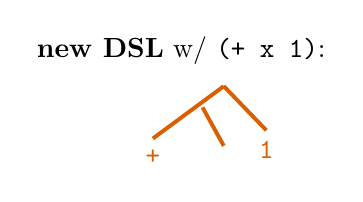
\begin{tikzpicture}[scale=0.9,line width=0.5mm]
          \node[align=center] at (0,0) {\textbf{new DSL} w/ \texttt{(+ x 1)}:};
          \begin{scope}[shift={(0.6,-0.5)}]
            \node[pop3](p1) at (-1,-1) {\texttt{+}};
            \node[pop3](n1) at (0.6,-0.9) {\texttt{1}};
            \node[pop3](a) at (0,-1) {\texttt{ }};
            \draw[pop3] (0,0) -- (p1.north);
            \draw[pop3] (0,0) -- (n1.north);
            \draw[pop3] (-0.3,-0.3) -- (a.north);
          \end{scope}
      \end{tikzpicture}};
      \draw [-> ] (c.south) -- (d.north);



      \begin{scope}[shift={(4,-8)},scale=0.6,line width=0.05mm]
        \node[latent,scale=0.7] at (3.5,3) (dx){DSL};
        \node[obs,scale=0.7] at ([yshift=-1.7cm,xshift=0cm]dx) (zp){prog};
        \node[obs,scale=0.7] at ([yshift=-1.45cm]zp) (xp) {task};
        \node[obs,scale=0.7] at ([xshift=1.5cm]zp) (zp1){prog};
        \node[obs,scale=0.7] at ([xshift=1.5cm]xp) (xp1) {task};
        \draw [->] (zp1.south) -- (xp1.north);
        \draw [->] (dx.south) -- (zp1.north);
        \node[obs,scale=0.7] at ([xshift=-1.5cm]zp) (zp1){prog};
        \node[obs,scale=0.7] at ([xshift=-1.5cm]xp) (xp1) {task};
        \draw [->] (zp1.south) -- (xp1.north);
        \draw [->] (dx.south) -- (zp1.north);
        \draw [->] (dx.south) -- (zp.north);
        \draw [->] (zp.south) -- (xp.north);
      \end{scope}


      \end{scope}


    
    %% center spiral
    \begin{scope}[shift={(3.25,-7.9)},scale=0.8]    
      \spiral{(3.5,1)}{3.5}
      \node[latent,scale=1] at (3.5,3) (dx){DSL};
      \node[latent,scale=1] at ([yshift=-1.7cm,xshift=0cm]dx) (zp){prog};
      \node[obs,scale=1] at ([yshift=-1.45cm]zp) (xp) {task};
      \node[latent,scale=1] at ([xshift=2cm]zp) (zp1){prog};
      \node[obs,scale=1] at ([xshift=2cm]xp) (xp1) {task};
      \draw [->] (zp1.south) -- (xp1.north);
      \draw [->] (dx.south) -- (zp1.north);
      \draw [->,red] (xp1.east) to[out = 30,in = -30] node(nn){} (zp1.east);
      
      \node[latent,scale=1] at ([xshift=-2cm]zp) (zp1){prog};
      \node[obs,scale=1] at ([xshift=-2cm]xp) (xp1) {task};
      \draw [->] (zp1.south) -- (xp1.north);
      \draw [->] (dx.south) -- (zp1.north);
      \draw [->,red] (xp1.east) to[out = 30,in = -30] node(nn){} (zp1.east);


      \draw [->,red] (xp.east) to[out = 30,in = -30] node(nn){} (zp.east);
      \draw [->] (dx.south) -- (zp.north);
      \draw [->] (zp.south) -- (xp.north);

      \node at ([yshift=-0.6cm]xp.south) {\legend};

    \end{scope}
    
  \end{tikzpicture}
  \caption{\textbf{Middle:} \system as a graphical model. Agent observes programming tasks (e.g., input/outputs for list processing or images for graphics programs), which it explains with latent programs, while jointly inferring a latent Domain Specific Language (DSL) capturing cross-program regularities. A neural network, called the \emph{recognition model} (red arrows) is trained to quickly infer programs with high posterior probability. \textbf{Top}: Wake phase infers programs while holding the DSL and recognition model fixed. \textbf{Left}: Sleep (Consolidation) phase infers DSL while holding the programs fixed by refactoring programs found during waking and extracting common components. \textbf{Right}: Sleep (Dreaming) phase trains recognition model to predict approximate posterior over programs conditioned on task. Trained on `Fantasies' (programs sampled from DSL) \& `Replays' (programs found during waking).}\label{threeCycles}
\end{figure}


\subsection{Wake: Solving tasks}\label{explorationSection}

During waking we enumerate programs from the DSL in decreasing order
of their probability according to the recognition model, and then
check if a program $p$ assigns positive probability to a task
($\probability[x|p] > 0$); if so, we incorporate $p$ into the frontier
$\mathcal{F}_x$ (Figure~\ref{neuralPipeline}).  We represent programs
as polymorphicly-typed $\lambda$-calculus expressions, a
representation closely resembling Lisp and functional languages like
Haskell and OCaml, including variables, conditionals, higher-order
recursive functions, and the ability to create new functions.

%% Our programs are all
%% strongly typed.  We use the Hindley-Milner polymorphic typing
%% system~\cite{pierce} which is used in functional programming languages
%% like OCaml and Haskell.  We now define DSLs:
%% \begin{definition}
%% A DSL $\mathcal{D}$ is a set of typed $\lambda$-calculus expressions.
%% A weight vector $\theta$ for a DSL $\mathcal{D}$ is a vector of $|\mathcal{D}| + 1$ real numbers:
%% one number for each DSL element $e\in \mathcal{D}$, written $\theta_e$ and controlling the probability of  $e$ occurring in a program,
%% and a weight controlling the probability of a variable occurring in a program, $\theta_{\text{var}}$.
%% \end{definition}
%% \noindent Together with its weight vector, a DSL defines a distribution over
%% programs, $\probability[p|\mathcal{D},\theta]$.  We define this
%% distribution by specifying a procedure for drawing samples from
%% $\probability[p|\mathcal{D},\theta]$ (Appendix~\ref{generativeAppendix}).
%% Care must be taken to ensure that variable scoping rules are obeyed
%% and that programs are well-typed.  We ensure well-typed programs by
%% performing Hindley-Milner type inference~\cite{pierce} during
%% sampling, and assume that each task is annotated with the type of the
%% program that will solve it.
%% Appendix~\ref{enumerationAppendix}
%% explains how we enumerate,
%% rather than sample,
%% programs generated by Algorithm~\ref{sampleProgram}.


Why enumerate, when the program synthesis community has invented many
sophisticated algorithms that search for programs?~\cite{solar2008program,schkufza2013stochastic,feser2015synthesizing,osera2015type,polozov2015flashmeta}.
We have two reasons:
(1) A key point of our work is that learning the DSL, along with a neural recognition model, can make program induction tractable, even if the search algorithm is very simple.
(2) Enumeration is a general approach that can be applied to any program induction problem. Many of these more sophisticated approaches require special conditions on
the space of  programs.
\begin{figure}
  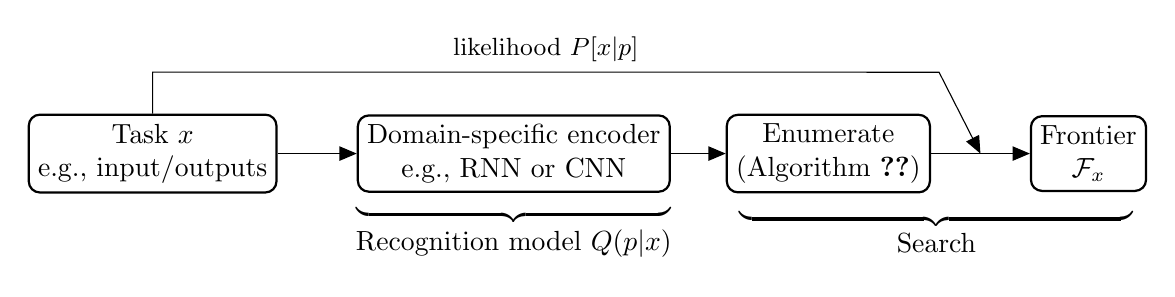
\begin{tikzpicture}[every node/.style={rounded corners,thick}]
    \node(x)[draw,align=center] at (0,0) {Task $x$\\e.g., input/outputs};
    \node(e)[draw, align=center] at ([xshift=3cm]x.east) {Domain-specific encoder\\
      e.g., RNN or CNN};
%    \node(m)[draw,align = center] at ([xshift=1.1cm]e.east) {MLP};%\\Output: $(|\mathcal{D}| + 2)\times(|\mathcal{D}| + 1)\times A$};
    \node[draw,align = center](s) at ([xshift=2cm]e.east) {Enumerate\\(Algorithm~\ref{recognitionSample})};
    \node(f)[draw,align = center] at ([xshift=2cm]s.east) {Frontier\\$\mathcal{F}_x$};

    \draw[->] (x.east) -- (e.west);
    \draw[->] (e.east) -- (s.west);
%    \draw[->] (m.east) -- node(p)[fill=white,align=center,midway,inner sep=0,outer sep=0,rotate=90]{\small $Q_{ijk}(x)$}(s.west);
    \draw[->] (s.east) -- (f.west);
    \draw[->] (x.north) -- ([yshift=15]x.north) -- node[above = 0pt,midway]{\small likelihood $\probability[x|p]$}([yshift=15,xshift=40]s.north) -- ($(s.east)!0.5!(f.west)$);
    \node[align=center] at ($(0,-1) + (e.center)$) {$\underbrace{\hspace{4cm}}_{\normalsize\text{\normalsize Recognition model $Q(p|x)$}}$};
    \node[align=center] at ($(s.west)!0.5!(f.east) + (0,-1)$) {$\underbrace{\hspace{5cm}}_{\text{\normalsize Search}}$};
  \end{tikzpicture}
  \caption{Neurally-guided program inference pipeline. Recognition model outputs distribution over program $Q(p|x)$. Program output by enumerative search incorporated into frontier if likelihood $\probability[x|p] > 0$}
  \label{neuralPipeline}
\end{figure}

%%   However, a drawback of   enumerative search  is that we have no
%% efficient means of solving for arbitrary constants that might occur in a
%% program. In Sec.~\ref{regressionSection},
%% we will show how to find programs with real-valued constants
%% by automatically differentiating through the program and setting the constants using gradient descent.
%% In Sec.~\ref{textSection}
%% we will show that the bottom-up neural recognition model can learn
%% which discrete constants should be included in a program.




\subsection{Consolidation-Sleep: Growing a Domain Specific Language}

The DSL offers a set of abstractions that allow an agent to concisely
express solutions to the tasks at hand. We automatically discover
these new abstractions by combining two ideas. First, we build on
techniques from the programming languages community to develop a new
algorithm for automatically refractoring programs, where this
refactoring exposes common reused subexpressions found across the
programs found during waking.  Second, we use this automatic refactoring
process to search for DSLs that maximally compress these programs by
incorporating reused subexpressions into the DSL.

Mathematically this compression takes the form of
finding the DSL maximizing $\int \lowerBound\;\mathrm{d}\theta$ (Sec.~\ref{overviewSection}).
We replace this marginal with an AIC approximation
and minimize the following expression,
which can be interpreted as a kind of compression:
\begin{equation}
\underbrace{-\log \probability[\mathcal{D}] + \min_{\theta}\Bigg(-\log
\probability[\theta|\mathcal{D}] + \|\theta\|_0}_{\text{Description length of }(\mathcal{D},\theta)} +\sum_{x\in
  X}\underbrace{-\log \sum_{p\in
  \mathcal{F}_x}\probability[x|p]\probability[p|\mathcal{D},\theta]}_{\text{Description length of programs for task }x}\Bigg)
\label{AIC}
  \end{equation}
At a high level, our approach is to search locally through the space 
of DSLs, proposing small changes to $\mathcal{D}$ until Eq.~\ref{AIC}
fails to decrease.  These small changes consist of introducing new
candidate $\lambda$-expressions into the DSL.

However, there is a snag with this simple approach:
whenever we add a new expression $e$ to the DSL,
the programs found during waking ($\left\{\mathcal{F}_x \right\}$)
are not written in terms of $e$.
Concretely, imagine we wanted to discover a new DSL procedure for doubling numbers,
after having found the programs
\code{(cons (+ 9 9) nil)} and \code{($\lambda$ (x) (+ (car x) (car x)))}.
As human programmers,
we can look at these pieces of code and recognize that,
if we define a new procedure called \code{double},
defined as \code{($\lambda$ (x) (+ x x))},
then we can rewrite the original programs as
\code{(cons (double 9) nil)} and \code{($\lambda$ (x) (double (car x)))}.
This process is a kind of refactoring
where a new subroutine is defined (\code{double})
and the old programs rewritten
in terms of the new subroutine.
Figure~\ref{mapFactor}A
diagrams this refactoring
process for a more complicated
setting,
where the agent must rediscover the higher-order function \code{map}
starting from the basics of Lisp and the Y-combinator.

We refine our objective to compress
\emph{refactorings} of the programs found during waking, minimizing
\begin{equation}
        -\log \probability[\mathcal{D}] + 
\min_{\theta}\Bigg(-\log \probability[\theta|\mathcal{D}] + \|\theta\|_0 +\sum_{x\in X} - \log \underbrace{\sum_{\substack{p:\\\exists p'\in \mathcal{F}_x: p\manyReduce p'}}}_{\text{Refactors }\mathcal{F}_x}\probability[x|p]\probability[p|\mathcal{D},\theta]\Bigg)
\label{factorObjective}
\end{equation}
where $p\manyReduce p'$ is the standard notation for ``expression $p$
evaluates to $p'$ by the rules of $\lambda$-calculus''~\cite{pierce}.
Equation~\ref{factorObjective} captures the idea that we want to add
new components to the DSL while jointly refactoring our old programs
in terms of these new components.  But this joint optimization is
intractable, because there are infinitely many ways of refactoring a
program.  To make refactoring tractable we first limit the degree to
which a piece of code can be refactored: rather than consider every
refactoring, we bound the number of $\lambda$-calculus evaluation
steps separating a refactoring from its original program.  Now the
number of refactoring this is finite but astronomically large: for the
example in Figure~\ref{mapFactor} there are approximately $10^{14}$
possible refactorings -- a quantity that grows exponentially both as a
function of program size and a function of the bound on evaluation
steps. How can we tame this combinatorial explosion?

A structure called a \textbf{version space
  algebra}~\cite{lau2001programming,mitchell1977version,polozov2015flashmeta}
neatly resolves this exponential growth.  A version space is a
tree-shaped data structure that compactly represents a large set of
programs and supports efficient set operations like union,
intersection, and membership checking.  In
Appendix~\ref{appendixVersion}, we give a dynamic program that takes
as input a program $p$ and then outputs a version space containing the
refactorings of $p$. Figure~\ref{mapFactor}B diagrams a subtree of a
version space containing refactorings of a small program. Our
technique is substantially more efficient than explicitly representing
the space of possible refactorings: for the example in
Figure~\ref{mapFactor}A, we represent the space of refactorings using
a version space with $10^6$ nodes, which encodes $10^{14}$
refactorings.










%% \textbf{Idea 1:} Limit the degree to which
%% a piece of code can be refactored.
%% Instead of considering every refactoring,
%% bound the number of $\lambda$-calculus evaluation steps
%% separating a refactoring from its original program.
%% Formally,
%% we define the set of $n$-step refactorings as:
%% \begin{equation}
%%   R_n(p) = \left\{p'\;:\;p'\underbrace{\reduce p''\reduce\cdots\reduce}_{\text{$\leq n$ times}} p \right\}
%% \end{equation}
%% where $p_1\reduce p_2$ is the standard notation for ``$p_1$ rewrites to $p_2$
%% in one step according to the rules of $\lambda$-calculus''~\cite{pierce}.
%% For example,
%% \begin{align*}
%%   \code{((lambda (x) (x x)) (lambda (y) y))}\reduce&\\
%%   \code{((lambda (y) y) (lambda (y) y))}\reduce&\\
%%   \code{(lambda (y) y)}&
%% \end{align*}
%% Returning to Equation~\ref{factorObjective},
%% this approximation gives the following objective:
%% \begin{equation}
%%         \log \probability[\mathcal{D}] + \argmax_{\theta}\Bigg(\log \probability[\theta|\mathcal{D}] - \|\theta\|_0 +\sum_{x\in X}\log \sum_{p\in \mathcal{F}_x}\probability[x|p]\max_{p'\in R_n(p)}\probability[p'|\mathcal{D},\theta]\Bigg)
%% \label{limitedObjective}
%%   \end{equation}
%% In practice, setting the number of refactoring steps $n$ to 3 suffices
%% to give a competent DSL learning algorithm.  Although the number of
%% refactorings is now finite, it is still prohibitively large, and in
%% fact grows exponentially quickly both as a function of $n$ and as a
%% function of the size of the program being refactored.  For example,
%% for the programs in Figure~\ref{mapFactor}, there are approximately
%% $10^{14}$ possible refactorings.  Next, we show how to tame this
%% exponential explosion.



%% In Appendix~\ref{appendixVersion}, we describe a dynamic program for
%% efficiently constructing a version space containing every $n$-step
%% refactoring.
%% This dynamic program, which we call $I\beta_n(p)$,
%% satisfies $\denotation{I\beta_n(p)} =  R_n(p)$.
%% In other words,
%% this dynamic program
%% builds a data structure
%% that represents the entire set of
%% refactorings -- but without having to explicitly enumerate all of the refactorings.

With this machinery in hand, we now have all the pieces needed to
learn a DSL (Algorithm~\ref{grammarInductionAlgorithm}).
The functions $I\beta(\cdot )$ and \textsc{refactor} construct
a version space from a program and extract the shortest program from a version space, respectively (Algorithm~\ref{grammarInductionAlgorithm}, lines 5-6, 14; see Appendix~\ref{appendixVersion}).
To define the prior distribution over $(\mathcal{D},\theta})$ (Algorithm~\ref{grammarInductionAlgorithm}, lines 7-8), we penalize the syntactic complexity of the $\lambda$-calculus expressions in the DSL, defining $    \probability[\mathcal{D}]\propto\exp(-\lambda\sum_{p\in \mathcal{D}}\text{size}(p) )$ where $\text{size}(p)$  measures the size of the syntax tree of program $p$,
  and $\lambda$ controls how strongly we regularize the size of the DSL.
  We place a symmetric Dirichlet prior over the weight vector $\theta$.

To appropriately score each proposed $\mathcal{D}$ we must reestimate
 the weight vector $\theta$ (Algorithm~\ref{grammarInductionAlgorithm}, line 7).
Although this  may seem 
very similar to estimating the parameters of a probabilistic context free grammar,
for which we have effective approaches like the Inside/Outside algorithm~\cite{international2000derivation},
our DSLs are context-sensitive due to the presence of variables
in the programs and also due to the polymorphic typing system.
Appendix~\ref{mapAppendix} derives a tractable MAP estimator for $\theta$.



\begin{algorithm}%[H]
  %\setcounter{algorithm}{2} % there are two algorithms in the main paper.
  \caption{DSL Induction Algorithm}
  \label{grammarInductionAlgorithm}
  \begin{algorithmic}[1]
    \State {\bfseries Input:} Set of frontiers $\{\mathcal{F}_x\}$
    %         \STATE \textbf{Hyperparameters:} Pseudocounts $\alpha$, regularization parameter $\lambda$
    \State \textbf{Output:} DSL $\mathcal{D}$, weight vector $\theta$
    \State $\mathcal{D}\gets$ every primitive in $\{\mathcal{F}_x\}$
    \While{true}         
    \State $\forall p\in \bigcup_{x}\mathcal{F}_x: $ $v_p\gets I\beta(p)$ \Comment{Construct a version space for each program}
    \State Define $L(\mathcal{D}',\theta) =  \prod_x \sum_{p\in \mathcal{F}_x} \probability[x|p]\probability[\text{\textsc{refactor}}(p|\mathcal{D}')|\mathcal{D}',\theta]$ \Comment{Likelihood if $(\mathcal{D}',\theta)$ were the DSL}
    \State Define $\theta^*(\mathcal{D}') = \argmax_\theta \probability[\theta|\mathcal{D}'] L(\mathcal{D}',\theta)$ \Comment{MAP estimate of $\theta$}
    \State Define $\text{score}(\mathcal{D}') = \log \probability[\mathcal{D}'] + L(\mathcal{D}',\theta^*) - \|\theta\|_0$ \Comment{objective function}
    \State components $\gets$ $\left\{\textsc{refactor}(v|\mathcal{D})\;:\;\forall x, \forall p\in \mathcal{F}_x, \forall v\in \text{children}(v_p) \right\}$ \Comment{Propose many new DSL components}
    \State proposals $\gets$ $\left\{\mathcal{D}\cup\left\{c \right\}\;:\;\forall c\in \text{components} \right\}$ \Comment{Propose many new DSLs}
    \State $\mathcal{D}'\gets \argmax_{\mathcal{D}'\in \text{proposals}}\text{score}(\mathcal{D}') $\Comment{Get highest scoring new DSL}
    \State \textbf{if }$\text{score}(\mathcal{D}') < \text{score}(\mathcal{D})$\textbf{ return }$\mathcal{D},\theta^*(\mathcal{D})$\Comment{No changes to DSL led to a better score}
    \State $\mathcal{D}\gets\mathcal{D}'$ \Comment{Found better DSL. Update DSL.}
    \State $\forall x\;:\;\mathcal{F}_x\gets\left\{\text{\textsc{refactor}}(p|\mathcal{D})\;:\; p\in \mathcal{F}_x\right\}$\Comment{Refactor frontiers in terms of new DSL}
    \EndWhile
  \end{algorithmic}
\end{algorithm}




\begin{figure*}
  \centering\begin{tikzpicture}[every node/.style={inner sep=1,outer sep=0,rounded corners,thick}]
  \node(p1)[draw,rounded corners,thick] at (-1,0) {
    \begin{tabular}{l}
      \texttt{(Y ($\lambda$ (r l) (if (nil? l) nil}\\
      \texttt{ (cons (+ (car l) (car l))}\\
      \phantom{\texttt{(cons }}\texttt{ (r (cdr l))))))}
    \end{tabular}
  };
  \node(r1)[draw,inner sep=0,outer sep=0] at ([yshift=-2.5cm]p1.south) {
    \begin{tabular}{l}
      \texttt{(}\orange{\texttt{($\lambda$ (f) (Y ($\lambda$ (r l) (if (nil? l)}}\\
      \phantom{(($\lambda$ (f) (Y ($\lambda$ (r l)}\orange{\texttt{nil}}\\
      \phantom{(($\lambda$ (f) (Y ($\lambda$ (r l)}\orange{\texttt{(cons (f (car l))}}\\
      \phantom{(($\lambda$ (f) (Y ($\lambda$ (r l)}\orange{\texttt{ (r (cdr l)))))))}}\\
      \texttt{ ($\lambda$ (z) (+ z z)))}
    \end{tabular}
  };

  \node(p2)[draw] at ([xshift=4.5cm]p1.east) {
    \begin{tabular}{l}
      \texttt{(Y ($\lambda$ (r l) (if (nil? l) nil}\\
      \texttt{ (cons (- (car l) 1)}\\
      \phantom{\texttt{(cons }}\texttt{ (r (cdr l))))))}
    \end{tabular}
    
  };
  \node(r2)[draw] at ([yshift=-2.5cm]p2.south) {
    \begin{tabular}{l}
      \texttt{(}\orange{\texttt{($\lambda$ (f) (Y ($\lambda$ (r l) (if (nil? l)}}\\
      \phantom{(($\lambda$ (f) (Y ($\lambda$ (r l)}\orange{\texttt{nil}}\\
      \phantom{(($\lambda$ (f) (Y ($\lambda$ (r l)}\orange{\texttt{(cons (f (car l))}}\\
      \phantom{(($\lambda$ (f) (Y ($\lambda$ (r l)}\orange{\texttt{ (r (cdr l)))))))}}\\
      \texttt{ ($\lambda$ (z) (- z 1)))}
    \end{tabular}

  };

  \draw [->] (p1.south)  --(r1.north) node[fill=white,midway,align=center] {refactor\\($\approx 10^{14}$ refactorings)};
  \draw [->] (p2.south)  --(r2.north) node[fill=white,midway,align=center] {refactor\\($\approx 10^{14}$ refactorings)};

  \node[draw](m) at (3,-6.5) {
    \begin{tabular}{l}
      \fbox{\textsc{map}} = \orange{\texttt{($\lambda$ (f) (Y ($\lambda$ (r l) (if (nil? l) nil}}\\
      \phantom{\texttt{\emph{map}} = \texttt{($\lambda$ (f) (Y ($\lambda$ (r l) (if }}\orange{\texttt{(cons (f (car l))}}\\
      \phantom{\texttt{\emph{map}} = \texttt{($\lambda$ (f) (Y ($\lambda$ (r l) (if }}\orange{\texttt{(r (cdr l))))))}}\\
      \code{(}\fbox{\textsc{map}}\code{ ($\lambda$ (z) (+ z z)))}\quad(program rewritten w/ new \fbox{\textsc{map}} primitive)\\
      \code{(}\fbox{\textsc{map}}\code{ ($\lambda$ (z) (- z 1)))}\quad(program rewritten w/ new \fbox{\textsc{map}} primitive)\\
    \end{tabular}      
  };
  \draw [->](r1.south)--(m.north);
  \draw [->](r2.south)--(m.north);
  \node[fill=white] at ([yshift=0.5cm]m.north) {\textbf{Compress (MDL/Bayes objective)}};

  \node(t1)[draw] at ([yshift=1.5cm]p1.north) {\begin{tabular}{ll}
      \textbf{Task}:&\texttt{(1 2 3)$\to$(2 4 6)}\\
      &\texttt{(4 3 4)$\to$(8 6 8)}
  \end{tabular}};
  \draw [->] (t1.south)  --(p1.north) node[fill=white,midway] {Wake: program search};
  \node(t2)[draw] at ([yshift=1.5cm]p2.north) {\begin{tabular}{ll}
      \textbf{Task}:&\texttt{(1 2 3)$\to$(0 1 2)}\\
      &\texttt{(4 3 4)$\to$(3 2 3)}
  \end{tabular}};
  \draw [->] (t2.south)  --(p2.north) node[fill=white,midway] {Wake: program search};

  \node(panelA)[ultra thick, rounded corners=0, inner sep=10,outer sep=10, draw, fit=(t1) (t2) (m) (r1) (r2)] {}; \node at ($(0.5,0) + (panelA.west |- panelA.north)$) {\textbf{A}};

  \footnotesize
  \begin{scope}[shift={(2,-11)}]  
    \node[draw, rounded corners](u1) at (0,0) {union};
    \node[draw, rounded corners](u2) at ($(0,-1) + (u1.south)$) {\code{(}union\code{ 1)}}; \draw (u1.south) -- (u2.north);
    \node[draw, rounded corners](u21) at ($(-1.3,-1) + (u2.south)$) {\code{(($\lambda$ (x) (x 1)) +)}}; \draw ([xshift=-0.2cm]u2.south) -- (u21.north);
    \node[draw, rounded corners](u22) at ($(2.3,-1) + (u2.south)$) {\code{(($\lambda$ (x) (+ x)) 1)}};  \draw ([xshift=-0.2cm]u2.south) -- (u22.north);

    \node[draw, rounded corners](u11) at ($(-1.75,-1) + (u1.south)$) {\code{(+ 1 1)}}; \draw (u1.south) -- (u11.north);
    \node[draw, rounded corners](u12) at ($(2.75,-1) + (u1.south)$) {\code{(($\lambda$ (x) (x 1 1)) +)}}; \draw (u1.south) -- (u12.north);

    \node(vs) at ($(u21.west)!0.5!(u12.east) + (0,-1.25)$) {$\underbrace{\hspace{8cm}}_{\text{\normalsize Subset of version space}}$};

    \node[anchor=north](p) at ($(-6,0) + (u2)$) {\normalsize $\underbrace{\texttt{(+ 1 1)}}_{\text{\normalsize  Program}}$};
    \draw[ultra thick,->] ($(0.5,0) + (p.east)$) -- ($(1.5,0) + (p.east)$);
    \node at ($(1,0.25) + (p.east)$) {Refactors};
    \node(g)[anchor=left] at ($(7,0) + (u12.east)$) {\includegraphics[width = 6cm]{figures/vs.eps}};
    \node(panelB)[ultra thick, rounded corners=0, inner sep=10,outer sep=10, draw, fit=(p) (u1) (vs) (g)] {}; \node at ($(0.5,0) + (panelB.west |- panelB.north)$) {\normalsize\textbf{B}}; 


    %% \node(panelC)[ultra thick, rounded corners=0, inner sep=8,outer sep=8, draw, fit=(g)] {}; \node at ($(0.5,0) + (panelC.west |- panelC.north)$) {\normalsize\textbf{C}}; 
  \end{scope}
  
  \end{tikzpicture}
  \caption{DSL learning as code refactoring. \textbf{Panel A:} For each task we discover programs during waking, then refactor the code from those programs to expose common subprograms (highlighted in \orange{orange}). Common subprograms are incorporated into the DSL when they increase a Bayesian objective. Intuitively, these new DSL components best compress the programs found during waking. \textbf{Panel B:} \# of possible refactorings grows exponentially with program size, so we represent refactorings using version spaces, which augment syntax trees with a \emph{union} operator whose children are themselves version spaces. Right graph: version spaces are exponentially more efficient than explicitly constructing set of refactorings. In this graph, refactored programs are of the form $1+1+\cdots  + 1$.}\label{mapFactor}
\end{figure*}


\subsection{Dream Sleep: Training a Neural Recognition Model}\label{recognitionSection}

During ``dreaming'' the system learns a recognition model that guides
program search.  It learns from (program, task) pairs drawn from two
sources of self-supervised data: \emph{replays} of programs discovered
during waking, and \emph{fantasies}, or programs drawn from the DSL.
Replays ensure that the recognition model is trained on the actual
tasks it needs to solve, and does not forget how to solve them.
Fantasies ensure that the recognition model has a large and highly
varied corpus of (program, task) pairs to learn from.

Formally, the recognition model $Q(p|x)$ should approximate the posterior
$\probability[p|\mathcal{D},\theta,x]$.
We can either train $Q$ to perform full posterior inference by minimizing the expected KL-divergence, $  \expect\left[\text{KL}\left(\probability[p|x,\mathcal{D},\theta]\|Q(p|x) \right) \right]$,
or we can train $Q$ to perform MAP inference
by maximizing $\expect\left[\max_{p\text{ maxing }\probability[\cdot |x,\mathcal{D},\theta]} \log Q(p|x) \right]$,
where in both cases the expectation is taken over tasks. Taking this expectation over the empirical distribution of tasks trains $Q$ on replays; taking it over samples from the generative model trains $Q$ on fantasies.
We define a pair of alternative objectives for the recognition model,
$\mathcal{L}^{\text{posterior}}$ and $\mathcal{L}^{\text{MAP}}$,
which either train $Q$ to perform full posterior inference or MAP inference, respectively.
These objectives combine replays and fantasies:
\begin{align*}
  \mathcal{L}^{\text{posterior}} &= \mathcal{L}_{\text{Replay}}^{\text{posterior}} + \mathcal{L}_{\text{Fantasy}}^{\text{posterior}}&
  \mathcal{L}^{\text{MAP}} &= \mathcal{L}_{\text{Replay}}^{\text{MAP}} + \mathcal{L}_{\text{Fantasy}}^{\text{MAP}}\\
  \mathcal{L}_{\text{Replay}}^{\text{posterior}}& = \expect_{x\sim X}\left[\sum_{p\in \mathcal{F}_x}
    \frac{\probability\left[x,p|\mathcal{D},\theta \right]\log Q(p|x)}{\sum_{p'\in \mathcal{F}_x}\probability\left[x,p'|\mathcal{D},\theta \right]}\right] &
  \mathcal{L}_{\text{Replay}}^{\text{MAP}}& = \expect_{x\sim X}\left[\max_{\substack{p\in \mathcal{F}_x\\p\text{ maxing }\probability[\cdot |x,\mathcal{D},\theta]}} \log Q(p|x) \right]  \\
  \mathcal{L}_{\text{Fantasy}}^{\text{posterior}} &= \expect_{(p,x)\sim(\mathcal{D},\theta) }\left[\log Q(p|x)\right]&
  \mathcal{L}_{\text{Fantasy}}^{\text{MAP}} &= \expect_{x\sim(\mathcal{D},\theta) }\left[\max_{\substack{p\\p\text{ maxing }\probability[\cdot |x,\mathcal{D},\theta]}}\log Q(p)\right]
\end{align*}
We maximize $\mathcal{L}^{\text{MAP}}$ rather than
$\mathcal{L}^{\text{posterior}}$ for two reasons:
$\mathcal{L}^{\text{MAP}}$ prioritizes the shortest program solving a
task, thus more strongly accelerating enumerative search during waking;
and, combined with our parameterization of $Q$, described next, we
will show that $\mathcal{L}^{\text{MAP}}$ forces the recognition model
to break symmetries in the space of programs
(Sec.~\ref{symmetricSection}).

\subsubsection{Parameterizing $Q$}\label{recognitionParameterization}

Broadly the literature contains two different approaches to
parameterizing conditional distributions over programs.  The first
approach~\cite{devlin2017robustfill,zavershynskyi2018naps} is to use a
recurrent network to predict the entire program token-by-token, which
has the advantage that, if the network is sufficiently powerful, it
can completely solve the synthesis problem.  The disadvantage is that
these models can perform poorly at out-of-sample
generalization~\cite{}, which is critical for our setting, as the
agent may need to solve new tasks that are qualitatively different
from the tasks it has solved so far.

%% Second, a powerful deep
%% recurrent network may be costly to sample or enumerate from --- so if
%% the network cannot easily solve a task, we cannot compensate with
%% rapid sampling or enumeration.  In contrast, state-of-the-art
%% enumerative program synthesizers evaluate millions of programs per
%% second~\cite{feser2015synthesizing}.

The second approach is to have $Q$ predict a fixed-dimensional weight
vector, which then biases a fast enumerator~\cite{balog2016deepcoder,ec2}
or sampler~\cite{menon2013machine}.  This approach can enjoy strong
out-of-sample generalization, because it can fall back on enumeration
or sampling when the target program is unlike the training programs.
A main drawback is that the neural net is deliberately handicapped,
and can only send so much information about the target program.

We adopt a middle ground between these two extremes.  Our recognition
model predicts a distribution over primitives in the DSL,
conditioned on the local context in the syntax tree of the
program. When predicting the next node to add to the syntax tree of a program,
the recognition model
conditions on the parent node, as well as
which argument is being generated.
This is a kind of `bigram' model over trees,
where the bigrams
take the form of (parent, child, argument index).
Figure~\ref{bg} diagrams this generative process and Algorithm~\ref{recognitionSample}
specifies a sampling procedure for $Q(\cdot |x)$.
This parameterization
has three main advantages:
(1) it supports fast enumeration
and sampling of programs,
because the
recognition model
only needs to run once for each task;
(2) it allows the recognition model to provide fine-grained
information about the structure of the target program;
and (3)
training this recognition model
causes it to learn to break symmetries in the space of programs,
described next.
\begin{figure}
\centering  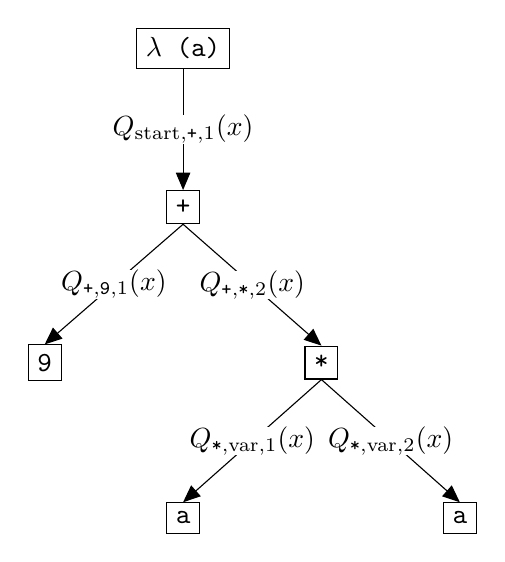
\begin{tikzpicture}%[every node/.style={inner sep=0,outer sep=0}]
    \node(l)[draw] at (0,0) {\texttt{$\lambda$ (a)}};
    \node(k)[draw] at ([yshift=-50]l.south) {\texttt{+}};
    \node(o)[draw] at ([xshift=-50,yshift=-50]k.south) {\texttt{9}};
    \node(m)[draw] at ([xshift=50,yshift=-50]k.south) {\texttt{*}};
    \node(x1)[draw] at ([xshift=50,yshift=-50]m.south) {\texttt{a}};
    \node(x2)[draw] at ([xshift=-50,yshift=-50]m.south) {\texttt{a}};

    \draw[->] (l.south)-- node[fill=white,align=center,midway,inner sep=0,outer sep=0]{$Q_{\text{start},\texttt{+},1}(x)$}(k.north);
    \draw[->] (k.south)--node[fill=white,align=center,midway,inner sep=0,outer sep=0]{$Q_{\texttt{+},\texttt{9},1}(x)$}(o.north);
    \draw[->] (k.south)--node[fill=white,align=center,midway,inner sep=0,outer sep=0]{$Q_{\texttt{+},\texttt{*},2}(x)$}(m.north);
    \draw[->] (m.south)--node[fill=white,align=center,midway,inner sep=0,outer sep=0]{$Q_{\texttt{*},\text{var},2}(x)$}(x1.north);
    \draw[->] (m.south)--node[fill=white,align=center,midway,inner sep=0,outer sep=0]{$Q_{\texttt{*},\text{var},1}(x)$}(x2.north);
\end{tikzpicture}
\caption{Parameterization of distribution over programs predicted by recognition model.
  Here the program (syntax tree shown above) is \texttt{($\lambda$ (a) (+ 9 (* a a )))}.
Each conditional distribution predicted by the recognition model is written $Q_{\text{parent},\text{child},\text{argument index}}(x)$, where $x$ is a task.}\label{bg}
\end{figure}

\subsubsection{Learning to break symmetries in program space}\label{symmetricSection}

A good DSL not only exposes high-level building blocks, but also
carefully restricts the ways in which those building blocks are
allowed to compose.  For example,
%% a DSL for list manipulation should
%% contain both the empty list and a routine for appending lists, but
%% should not allow appending the empty list.  Similarly 
a DSL for arithmetic should contain both addition and the number zero
but disallow adding zero.  These restrictions break symmetries in the
space of programs.  A bigram parameterization of the recognition
model, combined with the $\mathcal{L}^{\text{MAP}}$ training
objective, interact in a way that breaks symmetries in the program
space, allowing the agent to more efficiently explore the space of
programs.  This interaction occurs because the bigram parameterization
can disallow DSL primitives depending on their local syntactic
context, while the $\mathcal{L}^{\text{MAP}}$ objective forces all
probability mass onto a single member of a set of syntactically
distinct but semantically equivalent expressions
(Appendix~\ref{recognitionAppendix}).




We experimentally confirm this symmetry-breaking
behavior by training recognition models that minimize either
$\mathcal{L}^{\text{MAP}}$/$\mathcal{L}^\text{posterior}$ and which
use either a bigram parameterization/unigram\footnote{In the unigram variant $Q$ predicts a $|\mathcal{D}| + 1$-dimensional vector: $Q(p|x) = \probability[p|\mathcal{D},\theta_i = Q_i(x)]$,
  and was used in our prior work~\cite{ecc}} parameterization.
Figure~\ref{symmetry} shows the result of training $Q$ in these four regimes for a DSL containing \code{+}, \code{0}, and \code{1}
and then sampling programs.
On this particular run,
the combination of
bigrams and $\mathcal{L}^{\text{MAP}}$ learns to
avoid adding zero and associate addition to the right ---
different random initializations
lead to either right or left association.

\begin{figure}
  \begin{minipage}[c]{0.3\textwidth}
    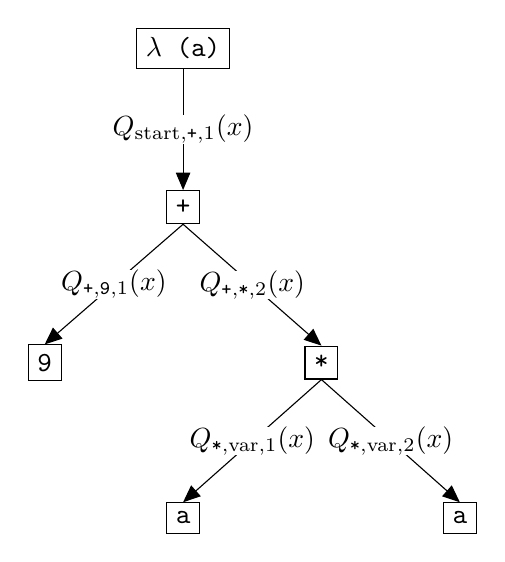
\begin{tikzpicture}%[every node/.style={inner sep=0,outer sep=0}]
    \node(l)[draw] at (0,0) {\texttt{$\lambda$ (a)}};
    \node(k)[draw] at ([yshift=-50]l.south) {\texttt{+}};
    \node(o)[draw] at ([xshift=-50,yshift=-50]k.south) {\texttt{9}};
    \node(m)[draw] at ([xshift=50,yshift=-50]k.south) {\texttt{*}};
    \node(x1)[draw] at ([xshift=50,yshift=-50]m.south) {\texttt{a}};
    \node(x2)[draw] at ([xshift=-50,yshift=-50]m.south) {\texttt{a}};

    \draw[->] (l.south)-- node[fill=white,align=center,midway,inner sep=0,outer sep=0]{$Q_{\text{start},\texttt{+},1}(x)$}(k.north);
    \draw[->] (k.south)--node[fill=white,align=center,midway,inner sep=0,outer sep=0]{$Q_{\texttt{+},\texttt{9},1}(x)$}(o.north);
    \draw[->] (k.south)--node[fill=white,align=center,midway,inner sep=0,outer sep=0]{$Q_{\texttt{+},\texttt{*},2}(x)$}(m.north);
    \draw[->] (m.south)--node[fill=white,align=center,midway,inner sep=0,outer sep=0]{$Q_{\texttt{*},\text{var},2}(x)$}(x1.north);
    \draw[->] (m.south)--node[fill=white,align=center,midway,inner sep=0,outer sep=0]{$Q_{\texttt{*},\text{var},1}(x)$}(x2.north);
\end{tikzpicture}
    \end{minipage}\hfill%
  \begin{tabular}{cll}
     \toprule
&     \multicolumn{1}{c}{Unigram}&\multicolumn{1}{c}{Bigram} \\\midrule
     $\mathcal{L}^{\text{posterior}}$&
     \begin{tabular}{l}
       \emph{Three samples:}\\
       \code{(+ 1 0)}\\
\code{(+ (+ 0 0)}\\\code{\phantom{(+ }(+ 1 0))}\\
\code{(+ 1 1)}
\\
63.0\% right-associative\\37.4\% \code{+0}'s
       \end{tabular}
     &
     \begin{tabular}{l}
       \emph{Three samples:}\\
       \code{0}\\
\code{(+ (+ (+ 0 0)}\\\code{\phantom{(+ (+} (+ 0 1)) 1)}\\
\code{1}\\
55.8\% right-associative\\31.9\% \code{+0}'s
       \end{tabular}
     \\\\
     $\mathcal{L}^{\text{MAP}}$&
     \begin{tabular}{l}
       \emph{Three samples:}\\
       \code{1}\\
       \code{(+ 1 (+ 1 (+ (+ 1 }\\\code{\phantom{(+ }(+ 1 1)) 1)))}\\
       \code{(+ (+ 1 1) 1)}
\\48.6\% right-associative\\
       0.5\% \code{+0}'s       
       \end{tabular}
     &
     \begin{tabular}{l}
       \emph{Three Samples:}\\
\code{(+ 1 (+ 1 (+ 1}\\\code{\phantom{(+ 1} (+ 1 (+ 1 1)))))}\\
\code{0}\\
\code{(+ 1 (+ 1 (+ 1 1)))}
       \\
       \textbf{97.9\% right-associative}\\
       2.5\% \code{+0}'s       
       \end{tabular}
\\    \bottomrule 
  \end{tabular}
  \caption{\textbf{Left:} Bigram parameterization of distribution over programs predicted by recognition model.
  Here the program (syntax tree shown above) is \texttt{($\lambda$ (a) (+ 9 (* a a )))}.
Each conditional distribution predicted by the recognition model is written $Q_{\text{parent},\text{child},\text{argument index}}(x)$, where $x$ is a task. \textbf{Right:} Agent learns to break symmetries in program space only when using both bigram parameterization and $\mathcal{L}^{\text{MAP}}$ objective, associating addition to the right and avoiding adding zero. \% right-associative calculated by drawing 500 samples from $Q$. $\mathcal{L}^{\text{MAP}}$/Unigram agent incorrectly learns to never generate programs with \code{0}'s, while $\mathcal{L}^{\text{MAP}}$/Bigram agent correctly learns that \code{0} should only be disallowed as an argument of addition. Tasked with building programs from \code{+}, \code{1}, and \code{0}. }\label{symmetry}
\end{figure}

\begin{figure}
\centering  \begin{tabular}{cll}
     \toprule
&     \multicolumn{1}{c}{Unigram}&\multicolumn{1}{c}{Bigram} \\\midrule
     $\mathcal{L}^{\text{posterior}}$&
     \begin{tabular}{l}
       \emph{Three samples:}\\
       \code{(+ 1 0)}\\
\code{(+ (+ 0 0) (+ 1 0))}\\
\code{(+ 1 1)}
\\
63.0\% right-associative; 37.4\% \code{+0}'s
       \end{tabular}
     &
     \begin{tabular}{l}
       \emph{Three samples:}\\
       \code{0}\\
\code{(+ (+ (+ 0 0) (+ 0 1)) 1)}\\
\code{1}\\
55.8\% right-associative; 31.9\% \code{+0}'s
       \end{tabular}
     \\\\
     $\mathcal{L}^{\text{MAP}}$&
     \begin{tabular}{l}
       \emph{Three samples:}\\
       \code{1}\\
       \code{(+ 1 (+ 1 (+ (+ 1 (+ 1 1)) 1)))}\\
       \code{(+ (+ 1 1) 1)}
\\48.6\% right-associative;
       0.5\% \code{+0}'s       
       \end{tabular}
     &
     \begin{tabular}{l}
       \emph{Three Samples:}\\
\code{(+ 1 (+ 1 (+ 1 (+ 1 (+ 1 1)))))}\\
\code{0}\\
\code{(+ 1 (+ 1 (+ 1 1)))}
       \\
       \textbf{97.9\% right-associative};
       2.5\% \code{+0}'s       
       \end{tabular}
\\    \bottomrule 
  \end{tabular}
  \caption{Agent learns to break symmetries in program space only when using both bigram parameterization and $\mathcal{L}^{\text{MAP}}$ objective, associating addition to the right and avoiding adding zero. \% right-associative calculated by drawing 500 samples from $Q$. $\mathcal{L}^{\text{MAP}}$/Unigram agent incorrectly learns to never generate programs with \code{0}'s, while $\mathcal{L}^{\text{MAP}}$/Bigram agent correctly learns that \code{0} should only be disallowed as an argument of addition. Tasked with building programs from \code{+}, \code{1}, and \code{0}. }\label{symmetry}
  \end{figure}



\section{Experiments}

\subsection{Programs that manipulate sequences}\label{sequences}
We first apply \system to two classic benchmark domains: list
processing and text editing. In both cases we solve tasks specified by
a few input/output examples, using a recurrent neural network for the
recognition model and starting with a generic functional programming
basis: \code{foldr}, \code{unfold}, \code{if}, \code{map},
\code{length}, \code{index}, \code{=}, \code{+}, \code{-}, \code{0},
\code{1}, \code{cons}, \code{car}, \code{cdr}, \code{nil}, and
\code{is-nil}.

\subsubsection{List Processing}\label{listSection}
We took 218 list manipulation tasks from our previous work~\cite{ec2},
each with 15 input/output examples.  In solving these tasks, the
system composed 16 new DSL components, and discovered multiple
higher-order functions, such as \code{filter} ($f_0$ in
Figure~\ref{initialExampleDSL}).  Each round of memory consolidation
built on components discovered in earlier sleep cycles --- for example
the agent first learns \code{filter}, uses filter to learn to take the
maximum element of a list, then uses that routine to learn a new
component for extracting the $n^{\text{th}}$ largest element of a
list, which it finally uses to learn how to sort a list of numbers
(Figure~\ref{initialExampleDSL}).  This incremental, modular learning
of deep hierarchies of DSL components occurs
because of the alternation between code writing and code refactoring.

%% \begin{figure}[b]\centering
%% \vspace{-0.5cm}  \begin{tabular}{lll}
%%     \toprule
%%     Name & Input & Output \\\midrule
%%     repeat-3 & [7\, 0] & [7\, 0\, 7\, 0\, 7\, 0] \\
%%     drop-3 & [0\, 3\, 8\, 6\, 4] & [6\, 4] \\
%%     rotate-2 & [8\, 14\, 1\, 9] & [1\, 9\, 8\, 14] \\
%%     count-head-in-tail & [1\, 2\, 1\, 1\, 3] & 2 \\
%%     keep-div-5 & [5\, 9\, 14\, 6\, 3\, 0] & [5\, 0] \\
%%     product & [7\, 1\, 6\, 2] & 84 \\
%%     \bottomrule
%%   \end{tabular}
%%   \captionof{table}{Some tasks in our list function domain.}\label{listExamples}\vspace{-0.5cm}
%% \end{figure}

\subsubsection{Text Editing}\label{textSection}
Synthesizing programs that edit text is a classic problem in the
programming languages and AI literatures~\cite{lau2001programming},
and algorithms that synthesize text editing programs ship in Microsoft
Excel~\cite{gulwani2011automatin}.  This prior work uses
hand-engineered DSLs and hand-engineered search strategies.  Here, we
will show that we can jointly learn both these ingredients and surpass
the state-of-the-art domain-general program synthesizers on a standard
text editing benchmark.

%% Because our enumerative search procedure cannot generate string %
%% constants, we instead enumerate programs with string-valued
%% parameters.  For example, to learn a program that prepends ``Dr.'', we
%% enumerate $\text{\code{(}}f_3\code{ string s)}$ -- where $f_3$ is the
%% learned appending primitive (Fig.~\ref{initialExampleDSL}) --- and then
%% define $\probability[x|p]$ by approximately marginalizing out the
%% string parameters via a simple dynamic program.
%% In Sec.~\ref{regressionSection}, we will use a similar trick to
%% synthesize programs containing real numbers, but using gradient
%% descent instead of dynamic programming.

We trained our system on 128 automatically-generated text editing tasks, with 4 input/output examples each.
We tested, but did not train, on the 108 text editing problems from the SyGuS~\cite{alur2016sygus} program synthesis competition. Before any learning,
\system solves 3.7\% of the problems within 10 minutes with an average search time of 235 seconds.
After learning,
it solves 79.6\%, and does so much faster,
solving them in an average of 40 seconds.
As of the 2017 SyGuS competition,
the best-performing synthesizer (CVC4) solves 82.4\% of the problems ---
but here, the competition conditions are 1 hour \& 8 CPUs per problem,
and with this more generous compute budget we
surpass
this previous
result and solve
84.3\% of the problems.
SyGuS additionally comes with a
different hand-engineered DSL \emph{for each text editing problem}. %\footnote{SyGuS text editing problems also prespecify the set of allowed string constants for each task. For these experiments, our system did not use this assistance.}
Here  we learned a single DSL
that applied generically to
all of the tasks,
and perform comparably to the best
prior work.

\subsection{Programs from visual input}
We consider three domains where the agent must infer a program from an
image (Figure~\ref{visualSpecs}).
\subsubsection{Programs that make plans and take actions}

We apply \system to two domains where the agent plans a series of actions
in order to draw a picture (Sec.~\ref{logoSection}) or build a tower out of blocks (Sec.~\ref{towerSection}).
For drawing pictures,
the agent controls a `pen' that it can pick up or place down while moving across a canvas.
For building towers,
the agent controls a `hand' that it moves through a simulated world while
placing down differently sized blocks.
For each of these domains,
the agent observes a target picture or block tower,
and must either draw the picture or build the tower.
The recognition model is a CNN that
observes an image of the target picture or tower.
The system is initially provided with two control flow operators:
\code{loop} (a `for' loop) and \code{get/set},
which saves and then restores the current state of the pen or hand.

\subsubsection{Programs that draw pictures}\label{logoSection}

Procedural visual concepts are studied across AI and cognitive science
--- Bongard problems~\cite{Moscow}, Raven's progressive
matrices~\cite{raven2003raven}, and Lake et al.'s BPL model of
omniglot~\cite{lake2015human} are prominent examples.  Here we take
inspiration from LOGO Turtle graphics~\cite{turtle}, and give our
agent the ability to control a pen, along with arithmetic operations
on angles and distances and simple control flow primitives.  We task
it with drawing a small corpus of images starting from this basis.

Inside its learned DSL we find interpretable parametric drawing
routines corresponding to the families of visual objects in its
training data, like polygons, circles, and spirals
(Figure~\ref{logoPrimitives}, left). It additionally learns more
abstract visual relationships, like rotational symmetry, which it
models by incorporating a higher-order function into its DSL
(Figure~\ref{logoPrimitives}, right).  This abstraction comes from
jointly compressing programs for all of the training images into its
DSL.

What does \system dream of?  Prior to learning samples from the DSL
are simple and largely unstructured (Figure~\ref{logoDreams}, left).
After training the samples become richly structured
(Figure~\ref{logoDreams}, right), compositionally recombining latent
building blocks and motifs acquired from the training data. This
offers a window into how the generative model bootstraps recognition
model training: as the DSL grows more finely tuned to the domain, the
neural net gets richer and more highly varied training data.


%% has primitives for moving the pen forward and rotating it (\code{move}),
%% picking the pen up and then putting it down (\code{pen-up}),
%% arithmetic operations on angles and distances,
%% and constants ($2\pi$, 0 through 9, and $\infty$\footnote{To ensure that programs terminate, we set $\infty = 20$}).

\begin{figure}\centering
  
\includegraphics[width = 0.3\textwidth]{figures/logo16.png}
  \includegraphics[width = 0.3\textwidth]{figures/tower9.png}
  \includegraphics[width = 0.3\textwidth]{figures/sr16.png}
  \caption{Three domains where the agent infers a program from visual input. \textbf{Left}: 16 (out of 145) LOGO graphics tasks. Agent writes a program controlling a `pen' that draws the target picture. \textbf{Middle}: 9 (out of 112) tower building tasks. Agent writes a program controlling a `hand' that builds the target tower. \textbf{Right}: 16 (out of 200) symbolic regression tasks. Agent writes a program containing continuous real numbers that fits the points along the curve.}\label{visualSpecs}
\end{figure}
\begin{figure}
\centering  \begin{tabular}{cc}
    \toprule
    Parametric drawing routines&Higher-order drawing routine\\\midrule
    \begin{tabular}{rl}
      Semicircle:& \raisebox{-.5\height}{\includegraphics[width = 0.3\textwidth]{figures/logo_primitives/logo_primitive_24.png}}\\
      Circles:
      &\raisebox{-.5\height}{\includegraphics[width = 0.3\textwidth]{figures/logo_primitives/logo_primitive_23.png}}\\
      Spiral:&\raisebox{-.5\height}{\includegraphics[width = 0.3\textwidth]{figures/logo_primitives/logo_primitive_25.png}}\\
      Greek Spiral:&\raisebox{-.5\height}{
\includegraphics[width = 0.3\textwidth]{figures/logo_primitives/logo_primitive_10.png}}\\
      S-Curves:&\raisebox{-.5\height}{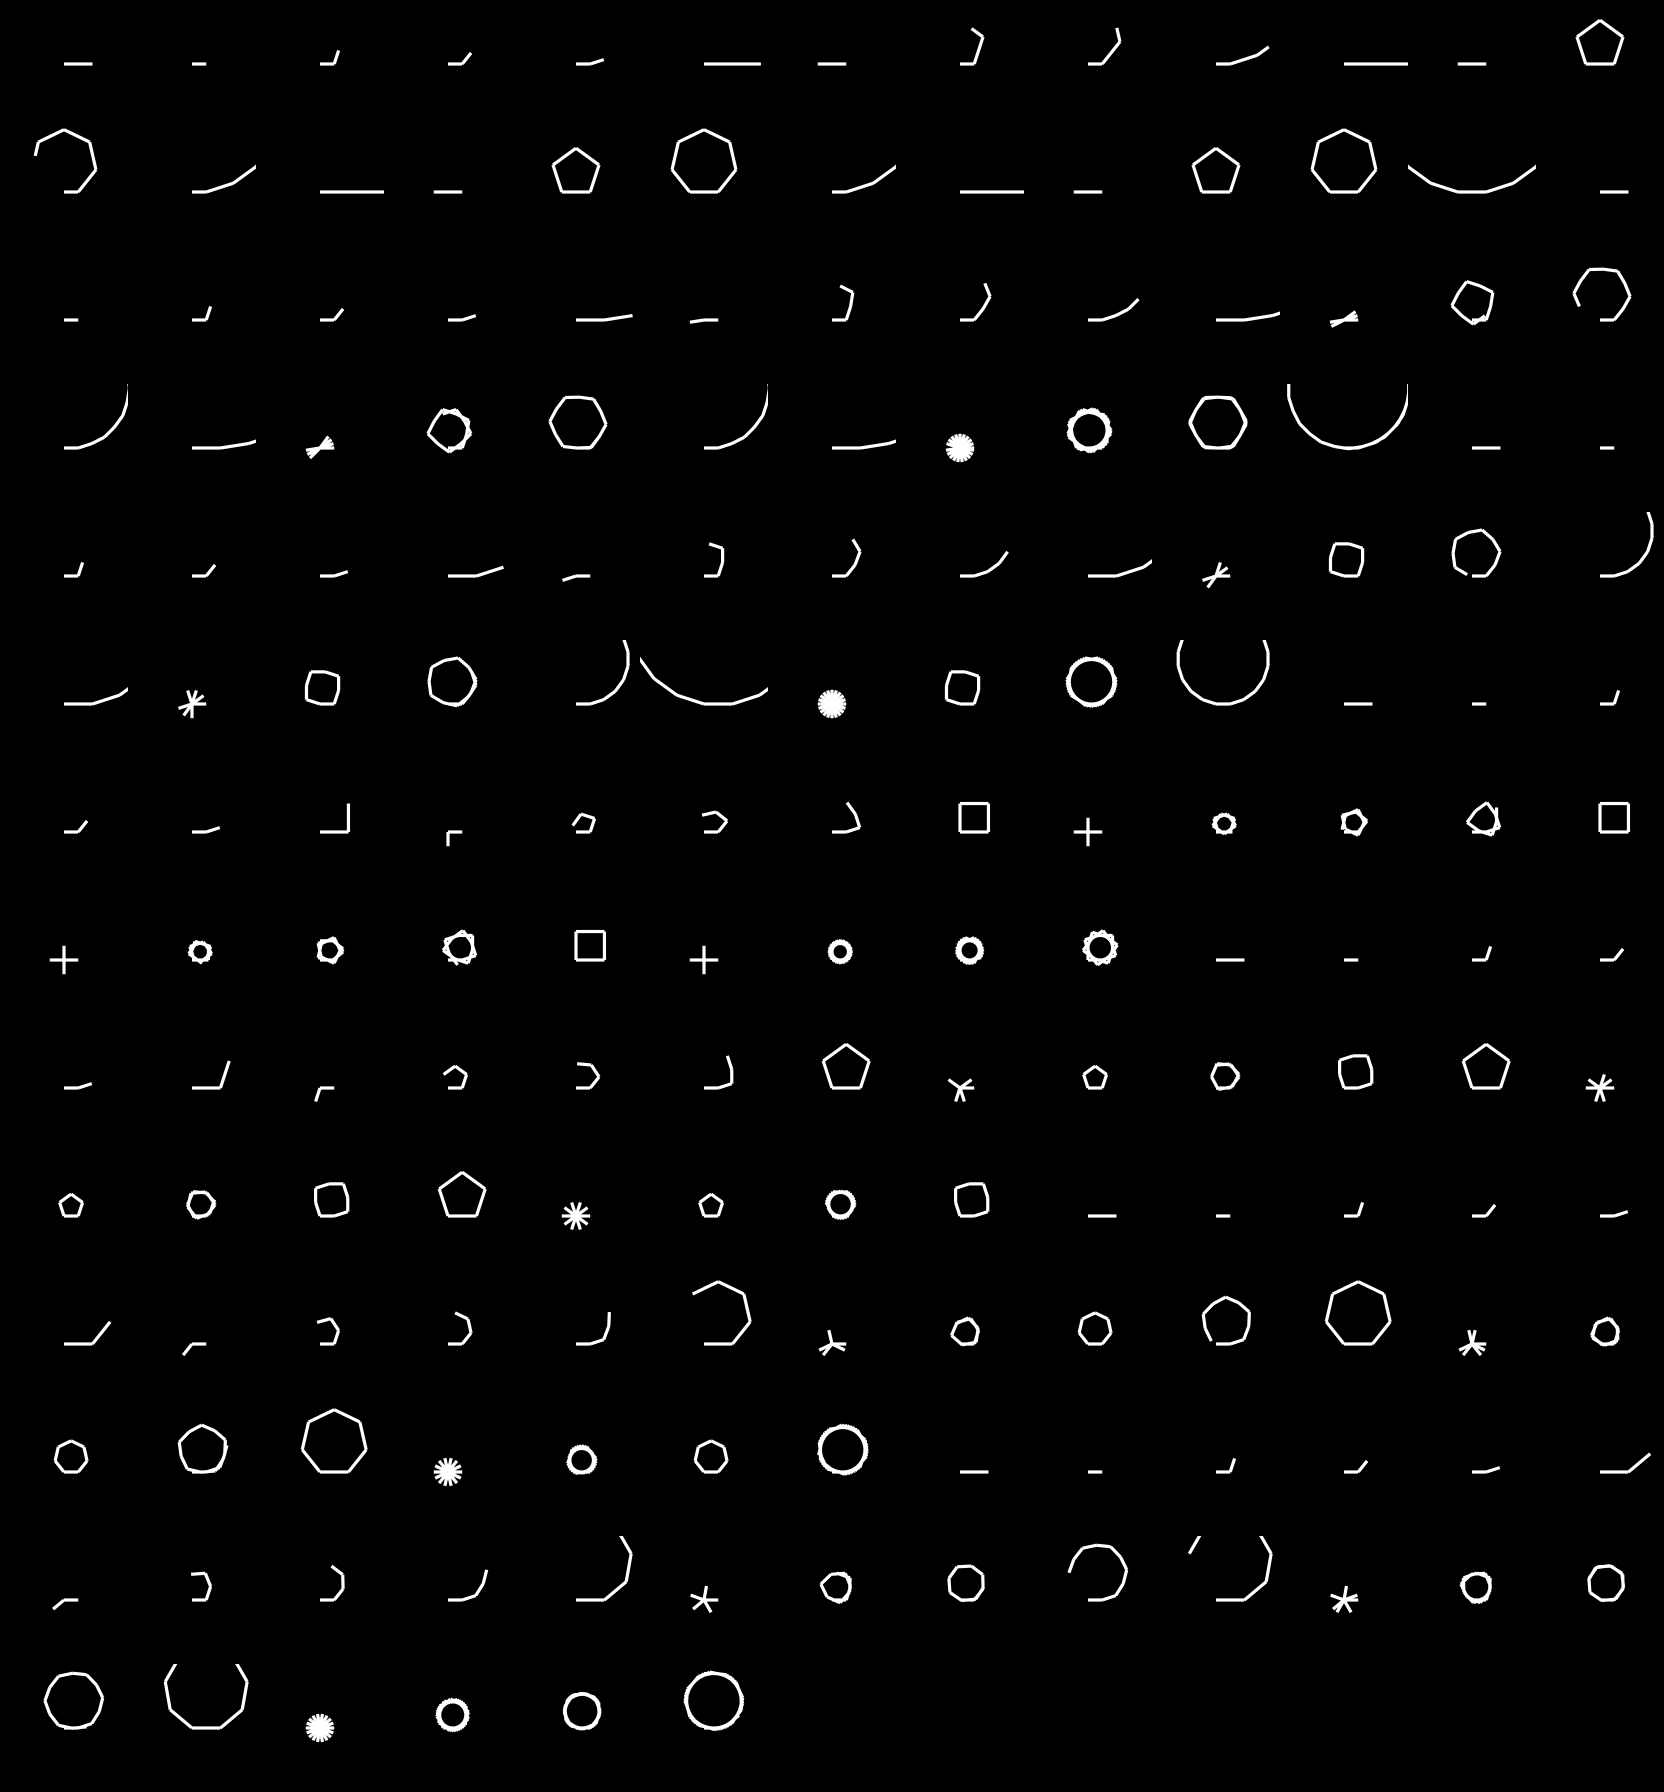
\includegraphics[width = 0.3\textwidth]{figures/logo_primitives/logo_primitive_11.png}}        \\
        Polygons \& Stars:
&\raisebox{-.5\height}{
\includegraphics[width = 0.3\textwidth]{figures/logo_primitives/logo_primitive_12.png}}
    \end{tabular}
    &
    \begin{tabular}{c}
      Rotational Symmetry:\\
          \includegraphics[width = 0.35\textwidth]{figures/rotationalmontage.png}
      \end{tabular}
    
    \\\bottomrule 
  \end{tabular}
  \caption{Example primitives learned by \system when trained on tasks in Figure~\ref{everyLogo}. Agent learns parametric routines for drawing families of curves (left) as well as subroutines that take entire programs as input (right). Each row of images on the left is the same code executed with different parameters. Each image on the right is the same code executed with different parameters and with a different subprogram provided as input.}\label{logoPrimitives}
  \end{figure}
\begin{figure}
\centering  \begin{tabular}{c|c}
      \includegraphics[width = 0.5\textwidth]{figures/initialDreams/montage.png}&
  \includegraphics[width = 0.5\textwidth]{figures/finalDreams/montage.png}
    \end{tabular}
  \caption{Dreams, or samples, from the DSL before (left) and after (right) training on tasks in Figure~\ref{everyLogo}. Blue: where the agent started drawing. Pink: where the agent ended drawing.}\label{logoDreams}
\end{figure}

\subsubsection{Building towers out of `Lego' blocks}\label{towerSection}

Inspired by the classic AI `copy task' --- where an agent must look at
an image of a tower made of toy blocks and re-create the
tower~\cite{towerCopy} --- we give \system 112 tower `copy tasks'
(Figure~\ref{towerTasks}).  Here the agent observes both an image of a
tower and the locations of each of its blocks, and must write a
program that plans how a simulated hand would build the tower.
These towers are built from Lego-style blocks
that snap together on a discrete grid.%%  (e.g., we do not model gravity
%% and discretize the coordinates of the 
%% blocks).
The system starts with the same control flow primitives as with
LOGO graphics,
and learns parametric `options' for building blocks towers (Figure~\ref{tower}),
inferring concepts like arches, staircases, bridges and brick walls.
\begin{figure}
  \begin{tabular}{cc}
    \toprule Example learned DSL components&Samples from DSL\\\midrule
    \begin{tabular}{rl}
      Brickwall&\begin{tabular}{l}
        \includegraphics[width = 5cm]{figures/tower/tower_dsl_bricks.png}
      \end{tabular}\\
      Bridge&\begin{tabular}{l}
        \includegraphics[width = 5cm]{figures/tower/tower_dsl_bridge.png}
      \end{tabular}\\
      Staircase&\begin{tabular}{l}
        \includegraphics[width = 5cm]{figures/tower/tower_dsl_staircase.png}
        \end{tabular}
    \end{tabular}&
    \begin{tabular}{l}
      \includegraphics[width = 5cm]{figures/tower/dreams.png}
      \end{tabular}
    \\\bottomrule 
    \end{tabular}
  \caption{\textbf{Left}: Three (out of 19) learned DSL components for building towers out of Lego-style blocks. These components act like parametric options~\cite{options},
    giving higher-level building blocks that the agent can use to plan. \textbf{Right}: 16 random samples, or `dreams', from learned DSL.}\label{tower}
\end{figure}



\subsubsection{Symbolic Regression}\label{regressionSection}
Here, the agent observes points along the curve of a function, and
must write a program that fits those points.  We initially equip our
learner with addition, multiplication, and division, and task it with
solving 200 symbolic regression problems, each either a polynomial or
rational function.  The recognition model is a convnet that observes
an image of the target function's graph (Fig.~\ref{visualSpecs},
rightmost) --- visually, different kinds of polynomials and rational
functions produce different kinds of graphs, and so the convnet can
look at a graph and predict what kind of function best explains it.  A
key difficulty, however, is that these problems are best solved with
programs containing real numbers.  Our solution to this difficulty is
to enumerate programs with real-valued parameters, and then fit those
parameters by automatically differentiating through the programs the
system writes and use gradient descent to fit the parameters.  We
define the likelihood model, $\probability[x|p]$, by assuming a
Gaussian noise model for the input/output examples, and penalize the
use of real-valued parameters using the
BIC~\cite{Bishop:2006:PRM:1162264}.

We learn a DSL containing 13 new functions, mainly templates for
different pieces of polynomials or ratios of polynomials.  The model
also learns to find programs minimizing the number of continuous
parameters --- for example, learning to represent linear functions
with \code{(* real (+ x real))}.  This phenomenon arises from our
Bayesian framing: both the generative model's bias toward shorter
programs, and the likelihood model's BIC penalty.


\subsection{Quantitative Results on Held-Out Tasks}\label{quantitative}
We evaluate  on held-out testing tasks,
measuring how many
tasks are solved and how long it takes to solve them (Fig.~\ref{learningCurves}).
Prior to any learning,
the system cannot find solutions for most of the tasks,
and those it does solve take a long time;
with more wake/sleep iterations,
we converge upon DSLs and recognition models 
more closely matching the domain.

%% We compare with ablations of our model on held out tasks.
%% The purpose of this ablation study is 
%% both to examine the role of each component of \systemEnding,
%% as well as to compare with
%% prior approaches in the literature:
%% a head-to-head
%% comparison of program synthesizers is complicated by the fact that
%% each system, including ours, makes idiosyncratic 
%% assumptions about the space of programs and the statement of tasks.

%% Nevertheless, much prior work can be modeled within our setup. 
%% We compare with the following ablations (Tbl~\ref{baselineComparisons};
%% Fig~\ref{learningCurves}):
%% \\\noindent \textbf{No NN:} lesions the recognition model.
%% \\\noindent \textbf{NPS}, which does not learn the DSL,
%% instead learning the recognition model
%% from samples drawn from the fixed DSL.
%% We call this NPS (Neural Program Synthesis)
%% because this is closest to how
%% RobustFill~\cite{devlin2017robustfill} and DeepCoder~\cite{balog2016deepcoder} are trained.
%% \\\noindent \textbf{SE}, which lesions the recognition model and restricts the DSL  learning algorithm to
%% only add \textbf{S}ub\textbf{E}xpressions of programs in the frontiers to the DSL. This is how most prior approaches have learned libraries of functions~\cite{Dechter:2013:BLV:2540128.2540316,DBLP:conf/icml/LiangJK10,DBLP:conf/ecai/LinDETM14}.
%% \\\noindent \textbf{PCFG}, which lesions the recognition model and does not learn the DSL,
%% but instead learns the parameters of the DSL ($\theta$), learning the parameters of a PCFG while not learning any of the structure.
%% \\\noindent \textbf{Enum}, which enumerates a frontier without any learning --- equivalently, our first search step.
%For each domain,
%% We are interested both in how many tasks the
%% agent can solve and how quickly it can find those solutions.
%% Tbl.~\ref{baselineComparisons}
%% compares our model against these alternatives.
%% We consistently
%% improve on the baselines,
%% and find that lesioning the recognition model
%% and lesioning it also slows down the convergence of the algorithm,
%% taking more iterations to reach a given number of tasks solved (Fig.~\ref{learningCurves}).
%% This supports a view of the recognition model as a way of amortizing the cost of search.

\begin{figure}
  \begin{tabular}{ccc}
    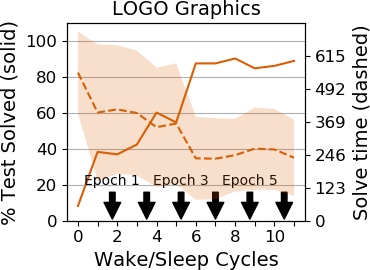
\includegraphics[width = 5cm]{figures/logoLearningCurve_batch.png}&
    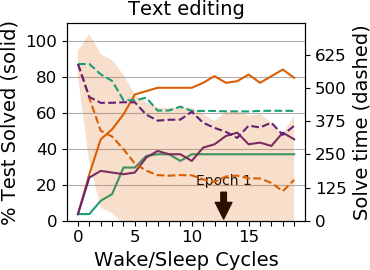
\includegraphics[width = 5cm]{figures/textLearningCurve_batch.png}&
    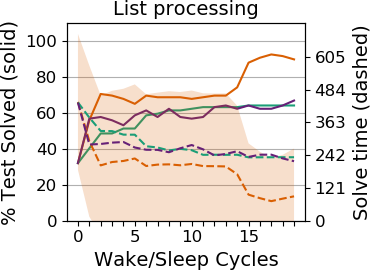
\includegraphics[width = 5cm]{figures/listLearningCurve_batch.png}\\\\
    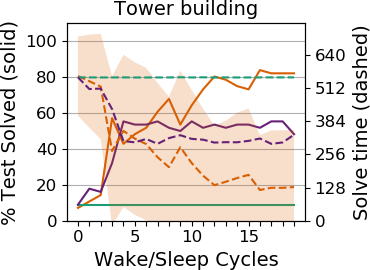
\includegraphics[width = 5cm]{figures/towerLearningCurve_batch.png}&
    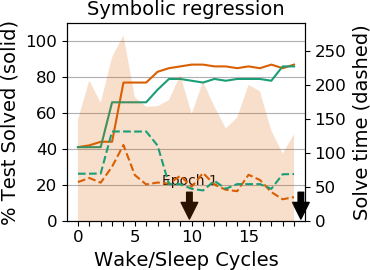
\includegraphics[width = 5cm]{figures/rationalLearningCurve_batch.png}&
  \end{tabular}
  \caption{}\label{learningCurves}
\end{figure}



\section{Discussion}

\subsection{Learning from Scratch}
A long-standing dream within the program induction community
is ``learning from scratch'': starting with a \emph{minimal} Turing-complete programming language,
and then learning to solve a wide swath of
induction problems~\cite{solomonoff1964formal,schmidhuber2004optimal,hutter2004universal,solomonoff1989system}.
All existing systems,
including ours,
fall far short of this dream,
and it is unclear (and we believe unlikely)
that this dream could ever be fully realized.
How far can we push in this direction?
``Learning from scratch'' is subjective, but a reasonable
starting point is the set of primitives provided in 1959
Lisp~\cite{mccarthy1960recursive}: these include
conditionals, recursion, arithmetic, and the 
list operators \code{cons}, \code{car}, \code{cdr}, and \code{nil}.
A  basic first goal is to start with
these primitives,
and then recover a DSL that
more closely resembles modern functional languages like Haskell and OCaml.
Recall (Sec.~\ref{sequences})
that we initially provided our system with functional programming routines like
\code{map} and \code{fold}.

We ran the following experiment: \system was given a subset of the
1959 Lisp primitives, and tasked with solving 22 programming
exercises. A key difference between this setup and our previous
experiments is that, for this experiment, the system is given
primitive recursion, whereas previously we had sequestered recursion
within higher-order functions like \code{map}, \code{fold}, and
\code{unfold}.

After running for 93 hours on 64 CPUs, our
algorithm solves these 22 exercises, along the way assembling a DSL
with a modern repertoire of
functional programming idioms and subroutines, including \code{map},
\code{fold}, \code{zip}, \code{unfold}, \code{index}, \code{length},
and  arithmetic operations like 
building lists of natural numbers between an interval (see  Appendix~\ref{appendixMcCarthy}).

We believe that program learners should \emph{not}
start from scratch,
but instead should start from
a rich, domain-agnostic
basis like those embodied in the standard libraries of modern  languages.
What this experiment shows is that \system doesn't \emph{need} to start from a rich basis,
and can in principle recover many of the amenities of modern programming systems,
provided it is given enough computational power and a suitable
spectrum of tasks.

\subsection{Program Induction as part of the generic AI toolkit}

Our aim with \system is both to show how learning can enable better
program synthesis, and to show how better program synthesis can be
more broadly useful for AI. How could a program induction approach to
AI become broadly useful across a diverse spectrum of AI problems ---
planning, natural language understanding, machine vision, causal
inference, and more?






\bibliography{main}
\bibliographystyle{plain}

\appendix

\section{Appendix}

\subsection{Generative model over programs}\label{generativeAppendix}
Algorithm~\ref{sampleProgram} gives a stochastic procedure for drawing samples from $\probability[\cdot |\mathcal{D},\theta]$.
It takes as input the desired type of the unknown program,
and performs type inference during
sampling to ensure that
the program has the desired type.
It also maintains a \emph{environment}
mapping variables to types,
which ensures
that lexical scoping rules are obeyed.
\begin{algorithm}
  \caption{Generative model over programs}
  \label{sampleProgram}
  \begin{algorithmic}[1]
    \State \textbf{function} sample$(\mathcal{D}, \theta, \tau)$:
    \State {\bfseries Input:} DSL $(\mathcal{D},\theta)$, type $\tau$
    \State \textbf{Output:} a program whose type unifies with $\tau$
    \State  \textbf{return }sample$'(\mathcal{D}, \theta, \varnothing, \tau)$

    \Statex
    \State \textbf{function} sample$'(\mathcal{D}, \theta, \mathcal{E}, \tau)$:
    \State {\bfseries Input:} DSL $(\mathcal{D},\theta)$, environment $\mathcal{E}$, type $\tau$\Comment{Environment $\mathcal{E}$ starts out as $\varnothing$}
    \State \textbf{Output:} a program whose type unifies with $\tau$
    \If{$\tau = \alpha\to\beta$}\Comment{Function type --- start with a lambda}
    \State var $\gets$ an unused variable name
    \State body $\sim$ sample$'(\mathcal{D},\theta,\{\text{var}:\alpha\}\cup\mathcal{E},\beta)$\Comment{Recursively sample function body}
    \State \textbf{return} \code{(lambda (}var\code{) }body\code{)}
    %\Endif
    \Else\Comment{Build an application to give something w/ type $\tau$}
    \State $\text{primitives} \gets \{p | &p: \tau' \in \mathcal{D}\cup\mathcal{E}$
    $\text{if }\tau\text{ can unify with yield}(\tau') \}$\Comment{Everything in scope w/ type $\tau$}
    \State $\text{variables}\gets\left\{p\;|\;p\in \text{primitives}\text{ and }p\text{ a variable} \right\}$
    \State Draw $e\sim \text{primitives}$, w.p. $\propto\begin{cases}
    \theta_e&\text{ if }e\in \mathcal{D}\\
    \theta_{var}/|\text{variables}|&\text{ if }e\in \mathcal{E}
    \end{cases}$
    \State Unify $\tau$ with yield$(\tau')$.\Comment{Ensure well-typed program}
    \State $\left\{\alpha_k \right\}_{k = 1}^K\gets\text{args}(\tau')$ 
    %   \State unify$(\tau,\beta)$
    \For{$k=1$ {\bfseries to} $K$}\Comment{Recursively sample arguments}
    \State $a_k\sim\text{sample}'(\mathcal{D},\theta,\mathcal{E},\alpha_k)$
    \EndFor
    \State \textbf{return} \code{(}$e\;a_1\; a_2\; \cdots\; a_K$\code{)}
    \EndIf
    \Statex
    \Statex\textbf{where:}
    \State yield$(\tau) = \begin{cases}
      \text{yield}(\beta)   &\text{ if }\tau = \alpha\to \beta\\
      \tau   &\text{ otherwise.}
    \end{cases}$ \Comment{Final return type of $\tau$}
    \State  args$(\tau) = \begin{cases}
      [\alpha] + \text{args}(\beta)   &\text{ if }\tau = \alpha\to \beta\\
      []   &\text{ otherwise.}
    \end{cases}$\Comment{Types of arguments needed to get something w/ type $\tau$}
  \end{algorithmic}
\end{algorithm}

\subsection{Enumerative program search}\label{enumerationAppendix}

Our current implementation of \system takes the simple and generic strategy of enumerating programs in
descending order of their probability under either $(\mathcal{D},\theta)$ or $Q(p|x)$.
Algorithm~\ref{sampleProgram} and~\ref{recognitionSample}
specify procedures for sampling
from these distributions,
but not for enumerating from them.
We combine two different enumeration strategies,
which allowed us to build a massively parallel program enumerator:
\begin{itemize}
\item \textbf{Best-first search:} Best-first search maintains a heap of
  partial programs ordered by their
  probability --- here a partial program means a program whose syntax tree
  may contain unspecified `holes'. Best-first search
  is guaranteed to enumerate programs in decreasing order of their probability,
  and has memory requirements that in general grow exponentially as a function of the description length of programs in the heap (thus linearly as a function of run time).
\item \textbf{Depth-first search:} Depth first search
  recursively explores the space of
  execution traces through Algorithm~\ref{sampleProgram} and~\ref{recognitionSample},
  equivalently maintaining a stack of partial programs.  
  In general it does not enumerate programs
  in decreasing order of probability,
  but has memory requirements that grow linearly as a function of the description length of the programs in the stack (thus logarithmically as a function of run time).
\end{itemize}

Our parallel enumeration algorithm (Algorithm~\ref{enumerationAlgorithm})
first performs a best-first search
until the best-first heap
is much larger than the number of CPUs.
At this point,
it switches to performing many depth-first searches in parallel,
initializing a depth first search
with one of the
entries in the best-first heap.
Because depth-first search does not
produce programs in decreasing order of their probability,
we wrap this entire procedure up into an outer loop
that first enumerates programs whose description length is between
$0$ to $\Delta$,
then programs with description length between $\Delta$ and $2\Delta$,
then $2\Delta$ to $3\Delta$, etc.,
until a timeout is reached.
This is similar in spirit to iterative deepening depth first search~\cite{Russell:2003:AIM:773294}.
 \begin{algorithm}
   \caption{Parallel enumerative program search algorithm }
   \label{enumerationAlgorithm}
   \begin{algorithmic}[1]
     \State \textbf{function} enumerate$(\mu, T, \text{CPUs})$:
     \State {\bfseries Input:} Distribution over programs $\mu$, timeout $T$, CPU count
     \State \textbf{Output:} stream of programs in approximately descending order of probability under $\mu$
     \State \textbf{Hyperparameter:} nat increase rate $\Delta$\Comment{We set $\Delta = 1.5$}
     \State lowerBound$\gets 0$
     \While{total elapsed time $ < T$}
     \State heap$\gets$newMaxHeap()\Comment{Heap for best-first search}
     \State heap.insert$(\text{priority} = 0,\text{value} = \text{empty syntax tree})$\Comment{Initialize heap with start state of search space}
     \While{$0 < |\text{heap}|\leq 10\times \text{CPUs}$}\Comment{Each CPU will get approximately 10 jobs (a partial program)}
     \State priority, partialProgram $\gets$ heap.popMaximum()
     \If{partialProgram is finished}\Comment{Nothing more to fill in in the syntax tree}
     \If{$\text{lowerBound}\leq -\text{priority} < \text{lowerBound} + \Delta$}
     \State \textbf{yield }partialProgram
     \EndIf
     \Else
     \For{child$\in $children(partialProgram)}\Comment{children$(\cdot )$ fills in next random choice in syntax tree.}
     \If{$-\log \mu(\text{child}) < \text{lowerBound} + \Delta$}\Comment{Child's description length small enough}
     \State heap.insert$(\text{priority} = \log \mu(\text{child}),\text{value} = \text{child})$
     \EndIf
     \EndFor
     \EndIf
     \EndWhile
     \State \textbf{yield from }ParallelMap$_\text{CPUs}(\text{depthFirst}(\mu,T - \text{elapsed time}, \text{lowerBound}, \cdot ), \text{heap.values()})$%\Comment{Launch parallel workers}
     \State $\text{lowerBound}\gets\text{lowerBound} + \Delta$\Comment{Push up lower bound on MDL by $\Delta$}
     \EndWhile
     \Statex
     \State \textbf{function} depthFirst$(\mu,T,\text{lowerBound},\text{partialProgram})$: \Comment{Each worker does a depth first search. Enumerates completions of partialProgram whose MDL is between lowerBound and $\text{lowerBound} + \Delta$}
     \State stack$\gets$[partialProgram]
     \While{$\text{total elapsed time} < T$ and $\text{stack}$ is not empty}
     \State partialProgram$\gets$stack.pop()
     \If{partialProgram is finished}
     \If{$\text{lowerBound}\leq-\log \mu(\text{partialProgram}) < \text{lowerBound} + \Delta$}
     \State \textbf{yield }partialProgram
     \EndIf
     \Else
     \For{$\text{child}\in \text{children}(\text{partialProgram})$}
     \If{$-\log \mu(\text{child}) < \text{lowerBound} + \Delta$}\Comment{Child's description length small enough}
     \State stack.push$(\text{child})$
     \EndIf
     \EndFor
     \EndIf

     \EndWhile
   \end{algorithmic}
 \end{algorithm}

 \subsection{Refactoring code with version spaces}\label{appendixVersion}
 Formally, a version space is either:
\begin{itemize}
\item A deBuijn\footnote{deBuijn indices are an alternative way of naming variables in $\lambda$-calculus. When using deBuijn indices, $\lambda$-abstractions are written \emph{without} a variable name, and variables are written as the count of the number of $\lambda$-abstractions up in the syntax tree the variable is bound to. For example, $\lambda x.\lambda y. (x\;y)$ is written $\lambda\lambda (\$1\;\$0)$ using deBuijn indices. See~\cite{pierce} for more details.} index: written $\$i$, where $i$ is a natural number
\item An abstraction: written $\lambda v$, where $v$ is a version space
\item An  application: written $(f \;x)$, where both  $f$ and $x$ are version spaces
\item A  union: $\uplus V$, where $V$ is a set of version spaces
\item The empty set, $\varnothing$
\item The set of all $\lambda$-calculus expressions, $\Lambda$
\end{itemize}
The purpose of a version space to compactly represent a set of programs.
We refer to this set as the \textbf{extension} of the version space:
\begin{definition}
  The \textbf{extension} of a version space $v$ is written $\denotation{v}$
  and is defined recursively as:
  \begin{align*}
    \denotation{\$i}& = \left\{\$i \right\}&
    \denotation{\lambda v}& = \left\{\lambda e : e\in \denotation{v} \right\}&
    \denotation{(v_1\; v_2)}& = \left\{(e_1\;e_2) : e_1\in \denotation{v_1},\;e_2\in \denotation{v_2} \right\}\\
    \denotation{\uplus V}& = \left\{e : v\in V,\;e\in \denotation{v} \right\}&
    \denotation{\varnothing}& = \varnothing&
    \denotation{\Lambda}& = \Lambda
    \end{align*}
\end{definition}
Version spaces also support efficient membership checking, which we
write as  $e\in \denotation{v}$.
Important for our purposes, it is also efficient to refactor the
members of a version space's extension in terms of a new DSL.
We define $\textsc{refactor}(v|\mathcal{D})$ inductively as:
\begin{align*}
  \textsc{refactor}(v|\mathcal{D}) &= \begin{cases}
    e\text{, if $e\in \mathcal{D}$ and $e\in \denotation{v}$. Exploits the fact that $\denotation{e}\in v$ can be efficiently computed.}\\
    \textsc{refactor}'(v|\mathcal{D})\text{, otherwise.}
  \end{cases}
\end{align*}\vspace{-\baselineskip}%
\begin{align*}
  \textsc{refactor}'(e|\mathcal{D})& = e\text{, if $e$ is a leaf}&%\\\nonumber
  \textsc{refactor}'(\lambda b|\mathcal{D}) &= \lambda \textsc{refactor}(b|\mathcal{D})\\\nonumber
  \textsc{refactor}'(f\;x|\mathcal{D}) &= \textsc{refactor}(f|\mathcal{D})\;\textsc{refactor}(x|\mathcal{D})&%\\\nonumber
  \textsc{refactor}'(\uplus V|\mathcal{D}) &= \argmin_{e\in \left\{\textsc{refactor}(v|\mathcal{D})\;:\;v\in V \right\}}\text{size}(e|\mathcal{D})\nonumber
  \end{align*}
where $\text{size}(e|\mathcal{D})$ for program $e$ and DSL $\mathcal{D}$
is the size of the syntax tree of $e$,
when members of $\mathcal{D}$ are counted as having size 1.
Concretely, $  \textsc{refactor}(v|\mathcal{D})$ calculates $\argmin_{p\in \denotation{v}}\text{size}(p|\mathcal{D})$.


Recall that our goal is to define an operator over version spaces, $I\beta_n$,
which calculates the set of $n$-step refactorings.
We define this operator in terms of another operator, $I\beta'$, which performs a single step of refactoring:
\begin{align*}
  I\beta_n(v)& = \uplus \left\{ \underbrace{I\beta'(I\beta'(I\beta'(\cdots}_{i \text{ times}} v))) \;:\; 0\leq i \leq n \right\}
\end{align*}
where
  \begin{align*}
    I\beta'(u)& = \uplus \left\{(\lambda b)v\;:\;v\mapsto b\in S_0(u)%\text{, when }v\not=\Lambda
    \right\}\cup
  \begin{cases}
    \text{if $u$ is a primitive or index or $\varnothing $:}&\varnothing\\
    \text{if $u$ is $\Lambda$:}&\left\{\Lambda \right\}\\
    \text{if $u = \lambda b$:}&\left\{\lambda I\beta'(b) \right\}\\
    \text{if $u = (f\;x)$:}&\left\{(I\beta'(f)\;x),\;(f\;I\beta'(x)) \right\}\\
    \text{if $u = \uplus V$:}&\left\{I\beta'(u')\;|\;u'\in V \right\}
  \end{cases}  
  \end{align*}
  where we have defined $I\beta'$
  in terms of another operator, $S_k:\text{VS}\to 2^{\text{VS}\times\text{VS}}$,
  whose purpose is to construct the set of
  substitutions that are refactorings of a program in a version space.
We define $S$ as:
  \begin{align*}
  S_k(v)& = \left\{\downshift{k}_0v\mapsto \$k \right\}\cup
  \begin{cases}
    \text{if $v$ is primitive:}&\left\{\Lambda\mapsto v \right\}\\    
    \text{if $v = \$i$ and $i < k$:}&\left\{\Lambda\mapsto \$i \right\}\\
    \text{if $v = \$i$ and $i\geq k$:}&\left\{\Lambda\mapsto \$(i + 1) \right\}\\
    \text{if $v = \lambda b$:}&\left\{v'\mapsto \lambda b' \;:\; v'\mapsto b'\in S_{k + 1}(b)  \right\}\\
    \text{if $v = (f\;x)$:}&\left\{v_1\cap v_2\mapsto (f'\;x') \;:\; v_1\mapsto f'\in S_k(f),\; v_2\mapsto x'\in S_k(x) \right\}\\
    \text{if $v = \uplus V$:}&\bigcup_{v'\in V}S_n(v')\\
    \text{if $v$ is $\varnothing$:}&\varnothing\\
    \text{if $v$ is $\Lambda$:}&\left\{\Lambda\mapsto\Lambda \right\}
  \end{cases}\\
  \downshift{k}_c \$i& = \$i\text{, when $i < c$}\\
  \downshift{k}_c \$i& = \$(i - k)\text{, when $i\geq c + k$}\\
  \downshift{k}_c \$i& = \varnothing \text{, when $c\leq i <  c + k$}\\
  \downshift{k}_c \lambda b &= \lambda\downshift{k}_{c + 1}b\\
  \downshift{k}_c (f\;x)& = (\downshift{k}_cf\;\downshift{k}_cx)\\
  \downshift{k}_c \uplus V& = \uplus \left\{\downshift{k}_c v \;|\;v\in V \right\}\\
  \downshift{k}_c v& = v\text{, when }v\text{ is a primitive or }\varnothing \text{ or }\Lambda
\end{align*}
where $\shift{k}$ is the shifting operator~\cite{pierce},
which adds $k$ to all of the free variables in a $\lambda$-expression or version space,
and we have defined a new operator, $\downshift$, whose purpose is to
undo the action of $\shift$.
We have written definitions recursively,
but implement them using a dynamic program:
we hash cons each version space,
and only calculate the operators $I\beta_n$,
$I\beta'$, and $S_k$ once per each version space.
%Refactoring is similarly done more quickly with dynamic programming (see Equation~\ref{FACTORING} for the recursive definition of \textsc{refactor}).

We now formally prove that $I\beta$ exhaustively enumerates the space of possible refactorings.
Our approach is to first prove that $S_k$ exhaustively enumerates
the space of possible substitutions that
could give rise to a program.
The following pair of technical lemmas are useful; both are easily proven by structural induction.
\begin{lemma}
  Let $e$ be a program or version space and $n$, $c$ be natural numbers. \\Then $\shift{-1}_{n + c}\shift{n + 1}_ce = \shift{n}_c e$,
  and in particular $\shift{-1}_{n}\shift{n + 1}e = \shift{n} e$.
\label{neutralizeShift}\end{lemma}
\begin{lemma}
  Let $e$ be a program or version space and $n$, $c$ be natural numbers. \\Then $\downshift{n}_{c}\shift{n}_ce =  e$,
  and in particular $\downshift{n}\shift{n}e =  e$.
  \label{neutralizeDown}
\end{lemma}


\begin{theorem}
  \textbf{Consistency of $S_n$}. \\If $(v\mapsto b)\in S_n(u)$ then
  for every $v'\in v$ and $b'\in b$ we have $\shift{-1}_n[\$n\mapsto \shift{1 + n}v']b'\in u$.
\end{theorem}
\begin{proof}
  Suppose $b = \$n$ and therefore, by the definition of $S_n$, also $v = \downshift{n}_0 u$.
  Invoking Lemmas~\ref{neutralizeShift} and~\ref{neutralizeDown}
  we know that $u = \shift{-1}_n\shift{n + 1}v$
  and so for every $v'\in v$ we have $\shift{-1}_n\shift{n + 1}v'\in u$.
  Because $b = \$n = b'$ we can rewrite this to $\shift{-1}_n[\$n\mapsto \shift{n + 1}v']b'\in u$.
  

  
  Otherwise assume $b\not= \$n$ and proceed by structural induction on $u$:

  \begin{itemize}
  \item If $u = \$i < n$ then we have to consider the case that $v = \Lambda$ and $b = u = \$i = b'$.
    Pick $v'\in \Lambda$ arbitrarily. Then $\shift{-1}_n[\$n\mapsto \shift{1 + n}v']b' = \shift{-1}_n\$i = \$i\in u$.
  \item If $u = \$i\geq n$ then we have consider the case that $v = \Lambda$ and $b = \$(i + 1) = b'$.
    Pick $v'\in \Lambda$ arbitrarily. Then $\shift{-1}_n[\$n\mapsto \shift{1 + n}v']b' = \shift{-1}_n\$(i + 1) = \$i\in u$.
  \item If $u$ is primitive then we have to consider the case that $v = \Lambda$ and $b = u = b'$.
    Pick $v'\in \Lambda$ arbitrarily. Then $\shift{-1}_n[\$n\mapsto \shift{1 + n}v']b' = \shift{-1}_nu = u\in u$.
  \item If $u$ is of the form $\lambda a$,
    then $S_n(u)\subset\left\{v\mapsto \lambda b\;|\; (v\mapsto b)\in S_{n + 1}(a) \right\}$.
    Let $v\mapsto \lambda b\in S_n(u)$.
    By induction for every $v'\in v$ and $b'\in b$ we have $\shift{-1}_{n + 1}[\$n\mapsto \shift{2 + n}v']b'\in a$,
    which we can rewrite to $\shift{-1}_{n}[\$n\mapsto \shift{1 + n}v']\lambda b'\in \lambda a = u$.
  \item If $u$ is of the form $(f\;x)$ then
    then $S_n(u)\subset\left\{v_f\cap v_x\mapsto (b_f\;b_x)\;|\; (v_f\mapsto b_f)\in S_{n}(f),\;(v_x\mapsto b_x)\in S_{n}(x) \right\}$.
    Pick $v'\in v_f\cap v_x$ arbitrarily.
    By induction for every $v_f'\in v_f$, $v_x'\in v_x$, $b_f'\in b_f$, $b_x'\in b_x$
    we have $\shift{-1}_{n}[\$n\mapsto \shift{1 + n}v_f'] b_f' \in f$ and $\shift{-1}_{n}[\$n\mapsto \shift{1 + n}v_x'] b_x' \in x$.
    Combining these facts gives
    $\shift{-1}_{n}[\$n\mapsto \shift{1 + n}v'] (b_f'\;b_x') \in (f\;x) = u$.
  \item If $u$ is of the form $\uplus U$ then
    pick $(v\mapsto b)\in S_n(u)$ arbitrarily.
    By the definition of $S_n$ there is a $z$ such that $(v\mapsto b)\in S_n(z)$,
    and the theorem holds immediately by induction.
  \item If $u$  is $\varnothing $ or $\Lambda$ then the theorem holds vacuously.
    \end{itemize}
\end{proof}
\begin{theorem}
  \textbf{Completeness of $S_n$}.\\
  If there exists programs $v'$  and $b'$, and a version space $u$, such that $\shift{-1}_n[\$n\mapsto \shift{1 + n}v']b'\in u$,
  then there also exists $(v\mapsto b)\in S_n(u)$ such that $v'\in v$ and $b'\in b$.
\end{theorem}
\begin{proof}
  As before we first consider the case that $b' = \$n$.
  If so then
  $\shift{-1}_n\shift{1 + n}v'\in u$ or (invoking Lemma~\ref{neutralizeShift}) that $\shift{n}v'\in u$
  and (invoking Lemma~\ref{neutralizeDown}) that $v'\in \downshift{n}u$.
  From the definition of $S_n$ we know that $(\downshift{n}u\mapsto \$n)\in S_n(u)$ which is what was to be shown.

  Otherwise assume that $b'\not=\$n$. Proceeding by structural induction on $u$:
  \begin{itemize}
  \item If $u = \$i$ then,
    because $b'$ is not $\$n$,
    we have $\shift{-1}_nb' = \$i$.
    Let $b' = \$j$,
    and so
    $$
    i =
    \begin{cases}
      j&\text{ if }j < n\\
      j - 1&\text{ if }j > n
    \end{cases}
    $$
    where $j = n$ is impossible because by assumption $b'\not=\$n$.
    
    If $j < n$ then
    $i = j$ and so $u = b'$.
    By the definition of $S_n$ we have
    $(\Lambda\mapsto \$i)\in S_n(u)$,
    completing this inductive step because $v'\in \Lambda$ and $b'\in \$i$.
    Otherwise assume $j > n$
    and so $\$i = \$(j - 1) = u$.
    By the definition of $S_n$ we have
    $(\Lambda\mapsto \$(i + 1))\in S_n(u)$,
    completing this inductive step because $v'\in \Lambda$
    and $b' = \$j = \$(i + 1)$.
  \item If $u$ is a primitive then,
    because $b'$ is not $\$n$,
    we have $\shift{-1}_nb' = u$,
    and so $b' = u$.
    By the definition of $S_n$ we have $(\Lambda\mapsto u)\in S_n(u)$
    completing this inductive step because $v'\in \Lambda$ and $b' = u$.
  \item If $u$ is of the form $\lambda a$ then,
    because of the assumption that $b'\not=\$n$,
    we know that $b'$ is of the form $\lambda c'$ 
    and that $\lambda \shift{-1}_{n + 1}[\$(n + 1)\mapsto \shift{2 + n}v']c'\in \lambda a$.
    By induction this means that there is a $(v\mapsto c)\in S_{n + 1}(a)$
    satisfying $v'\in v$ and $c'\in c$.
    By the definition of $S_n$ we also know that
    $(v\mapsto  \lambda c)\in S_n(u)$,
    completing this inductive step because $b' = \lambda c'\in \lambda c$.
  \item If $u$ is of the form $(f\;x)$
    then,
    because of the assumption that $b'\not=\$n$,
    we know that $b'$ is of the form $(b_f'\;b_x')$
    and that both
    $\shift{-1}_n[\$n\mapsto \shift{1 + n}v']b_f'\in f$ and $\shift{-1}_n[\$n\mapsto \shift{1 + n}v']b_x'\in x$.
    Invoking the inductive hypothesis twice
    gives a
    $(v_f\mapsto b_f)\in S_n(f)$ satisfying $v'\in v_f$, $b_f'\in b_f$
    and a
    $(v_x\mapsto b_x)\in S_n(x)$ satisfying $v'\in v_x$, $b_x'\in b_x$.
    By the definition of $S_n$
    we know that $(v_f\cap v_x\mapsto b_f\;b_x)\in S_n(u)$
    completing the inductive step because $v'$ is guaranteed to be
    in both $v_f$ and $v_x$ and we know that
    $b' = (b_f'\;b_x')\in (b_f\;b_x)$.

  \item If $u$ is of the form $\uplus U$
    then there must be a $z\in U$ such that $\shift{-1}_n[\$n\mapsto \shift{1 + n}v']b'\in z$.
    By induction there is a $(v\mapsto b)\in S_n(z)$ such that $v'\in v$ and $b'\in v$.
    By the definition of $S_n$ we know that $(v\mapsto b)$ is also in $S_n(u)$ completing the inductive step.
  \item If $u$  is $\varnothing $ or $\Lambda$ then the theorem holds vacuously.    
    \end{itemize}
\end{proof}

From these results the consistency and completeness of $I\beta$ follows:
\begin{theorem}
  \textbf{Consistency of $I\beta'$.}\\
  If $p\in \denotation{I\beta'(u)}$ then there exists $p'\in \denotation{u}$ such that $p\reduce p'$.
\end{theorem}
\begin{proof}
  Proceed by structural induction on $u$. If $p\in \denotation{I\beta'(u)}$ then, from the definition of $I\beta'$ and $\denotation{\cdot }$, at least one of the following holds:
  \begin{itemize}
  \item Case $p = (\lambda b')v'$ where $v'\in v$, $b'\in b$, and $v\mapsto b\in S_0(u)$:
    From the definition of $\beta$-reduction we know that $p\reduce \shift{-1}[\$0\mapsto \shift{1}v']b'$.
    From the consistency of $S_n$ we know that $\shift{-1}[\$0\mapsto \shift{1}v']b'\in u$.
    Identify $p' = \shift{-1}[\$0\mapsto \shift{1}v']b'$.
  \item Case $u = \lambda b$ and $p = \lambda b'$
    where $b'\in \denotation{I\beta'(b)}$:
    By induction there exists $b''\in \denotation{b}$ such that $b'\reduce b''$.
    So $p \reduce \lambda b''$.
    But $\lambda b''\in \denotation{\lambda b} = \denotation{u}$,
    so identify $p' = \lambda b''$.
  \item Case $u = (f\; x)$ and $p = (f'\; x')$ where $f'\in \denotation{I\beta'(f)}$ and $x'\in \denotation{x}$:
    By induction there exists $f''\in \denotation{f}$
    such that $f'\reduce f''$.
    So $(f'\;x')\reduce (f''\;x')$.
    But $(f''\;x')\in \denotation{(f\;x)} = \denotation{u}$,
    so identify $p' = (f''\;x')$.
  \item  Case $u = (f\; x)$ and $p = (f'\; x')$ where $x'\in \denotation{I\beta'(x)}$ and $f'\in \denotation{f}$: Symmetric to the previous case.
  \item Case $u = \uplus U$ and $p \in \denotation{I\beta'(u')}$ where $u'\in U$:
    By induction there is a $p'\in \denotation{u'}$ satisfying $p'\reduce p$.
    But $\denotation{u'}\subseteq \denotation{u}$, so also $p'\in \denotation{u}$.
  \item Case $u$ is an index, primitive, $\varnothing$, or $\Lambda$: The theorem holds vacuously.    
    \end{itemize}  
\end{proof}
\begin{theorem}
  \textbf{Completeness of $I\beta'$.}\\
  Let $p\reduce p'$ and $p'\in \denotation{u}$.
  Then $p\in \denotation{I\beta'(u)}$.
\end{theorem}
\begin{proof}
  Structural induction on $u$.
  If $u = \uplus V$
  then there is a $v\in V$
      such that $p' \in \denotation{v}$;
      by induction on $v$ combined with the definition of $I\beta'$ we have $p\in \denotation{I\beta'(v)}\subseteq \denotation{I\beta'(u)}$,
      which is what we were to show.
      Otherwise assume that $u\not=\uplus V$.
  
  From the definition of $p\reduce p'$
  at least one of these cases must hold:
  \begin{itemize}
  \item Case $p = (\lambda b')v'$ and $p' = \shift{-1}[\$0\mapsto \shift{1}v']b'$:
    Using the fact that $\shift{-1}[\$0\mapsto \shift{1}v']b'\in \denotation{u}$, we can invoke the completeness of $S_n$ to construct a $(v\mapsto  b)\in S_0(u)$
    such that $v'\in \denotation{v}$
    and $b'\in \denotation{b}$.
    Combine these facts with the definition of $I\beta'$
    to get
    $p = (\lambda b')v'\in \denotation{(\lambda b)v}\subseteq I\beta'(u)$.
  \item Case $p = \lambda b$ and $p' = \lambda b'$ where
    $b\reduce b'$:
    Because $p' = \lambda b'\in \denotation{u}$
    and by assumption $u\not=\uplus V$,
    we know that $u = \lambda v$ and $b'\in \denotation{v}$. By
    induction $b\in \denotation{I\beta'(v)}$.
    Combine with the definition of $I\beta'$ to get $p = \lambda b \in \denotation{\lambda I\beta'(v)}\subseteq \denotation{I\beta'(u)}$.
  \item Case $p = (f\;x)$ and $p' = (f'\;x)$ where $f\reduce f'$:
    Because $p' = (f'\;x)\in \denotation{u}$
    and by assumption $u\not=\uplus V$
    we know that $u = (a\;b)$
    where $f'\in \denotation{a}$
    and $x\in \denotation{b}$.
    By induction on $a$
    we know
    $f\in \denotation{I\beta'(a)}$.
    Therefore
    $p = (f\;x)\in \denotation{(I\beta'(a)\; b)}\subseteq\denotation{I\beta'((a\;b))}\subseteq\denotation{I\beta'(u)}$.
  \item Case $p = (f\;x)$ and $p' = (f\;x')$ where $x\reduce x'$: Symmetric to the previous case.    
  \end{itemize}
\end{proof}
Finally we have our main result:
\begin{theorem}
  \textbf{Consistency and completeness of $I\beta_n$.}
  Let $p$ and $p'$
  be programs.
  Then $p\underbrace{\reduce q\reduce\cdots\reduce}_{\text{$\leq n$ times}} p'$  if and only
  if $p\in \denotation{I\beta_n(p')}$.
\end{theorem}
\begin{proof}
  Induction on $n$.

  If $n = 0$
  then $\denotation{I\beta_n(p')} = \left\{p \right\}$
  and $p = p'$;
  the theorem holds immediately. Assume $n > 0$.
  
  If $p\underbrace{\reduce q\reduce\cdots\reduce}_{\text{$\leq n$ times}} p'$
  then $q\underbrace{\reduce\cdots\reduce}_{\text{$\leq n - 1$ times}} p'$;
  induction on $n$
  gives $q\in \denotation{I\beta_{n - 1}(p')}$.
  Combined with $p\reduce q$ we can invoke the completeness of $I\beta'$
  to get $p\in \denotation{I\beta'(I\beta_{n - 1}(p'))}\subset\denotation{I\beta_n(p')}$.
  
  If $p\in \denotation{I\beta_n(p')}$
  then
  there exists a $i\leq n$
  such that $p\in \denotation{\underbrace{I\beta'(I\beta'(I\beta'(\cdots}_{i \text{ times}} p')))}$.
  If $i = 0$
  then $p = p'$ and $p$ reduces to $p'$ in $0\leq n$ steps.
  Otherwise $i > 0$
  and $p\in \denotation{I\beta'(\underbrace{I\beta'(I\beta'(\cdots}_{i - 1 \text{ times}} p'))}$.
  Invoking the
  consistency of $I\beta'$
  we know that $p\reduce q$
  for a program $q\in \denotation{\underbrace{I\beta'(I\beta'(\cdots}_{i - 1 \text{ times}} p'))}\subseteq\denotation{I\beta_{i - 1}(p')}$.
  By induction $q\underbrace{\reduce\cdots\reduce}_{\text{$\leq i - 1$ times}} p'$,
  which combined with $p\reduce q$
  gives  $p\underbrace{\reduce q\reduce\cdots\reduce}_{\text{$\leq i\leq n$ times}} p'$.  
\end{proof}

%% First observe that
%% we do not \emph{enumerate} every refactoring,
%% but only those for which every expression of the form $(\lambda x.b)v$ has
%% $x$ free in $b$.
%% For example, we do not refactor $\code{+}$ into $(\lambda x. \code{+})v$ where $v$ is arbitrary,
%% because there are infinitely many such refactorings.
%% Define the following relation,
%% which captures this restricted kind of
%% refactoring:
%% \begin{gather*}
%%   \frac{f\reduce^\sim f'}{f\;x \reduce^\sim f'\;x}\qquad
%%   \frac{x\reduce^\sim x'}{f\;x \reduce^\sim f\;x'}\qquad
%%   \frac{b\reduce^\sim b'}{\lambda b \reduce^\sim \lambda b'}\qquad
%%   \frac{\$0 \text{ occurs free in }b}{(\lambda b)v\reduce^\sim \shift{-1}[\$0\mapsto \shift{1}v]b}
%%   \end{gather*}
%% \begin{theorem}
%%   \textbf{Completeness of $I\beta'$.}
%%   Let $v$ be a version space and let $p\in v$.
%%   If $p'\reduce^\sim p$
%%   then $p'\in I\beta'(v)$.
%% \end{theorem}
%% \begin{proof}
%%   We know (from the definition of $\reduce^\sim$) that $p'$ and $p$ differ only
%%   in that there exists a single subexpression in
%%   $p'$ of the form $(\lambda b)v$
%%   where that subexpression occurs in
%%   $p$ as $\shift{-1}[\$0\mapsto \shift{1}v]b$.
%%   From Theorem~\ref{}
%% \end{proof}


\subsubsection{Computational complexity of DSL learning}

How long does each update to the DSL in
Algorithm~\ref{grammarInductionAlgorithm} take?  Constructing the
version spaces takes time linear in the number of programs (written
$P$) in the frontiers (Algorithm~\ref{grammarInductionAlgorithm}, line
5), and, in the worst case, exponential time as a function of the
number of refactoring steps $n$ --- but we bound the number of steps
to be a small number (typically $n = 3$).  Writing $V$ for the number
of version spaces, this means that $V$ is $O(P2^n)$.  The number of
proposals (line 10) is linear in the number of distinct version
spaces, so is $O(V)$.  For each proposal we have to refactor every
program (line 6), so this means we spend $O(V^2) = O(P^22^n)$ per DSL
update.  In practice this quadratic dependence on $P$ (the number of
programs) is prohibitively slow.  We now describe a linear time
approximation to the refactor step in
Algorithm~\ref{grammarInductionAlgorithm} based on beam search.

For each version space $v$ we calculate a \emph{beam}, which is a
function from a DSL $\mathcal{D}$ to a shortest program in
$\denotation{v}$ using primitives in $\mathcal{D}$.  Our strategy will
be to only maintain the top $B$ shortest programs in the beam;
throughout all of the experiments in this paper, we set $B = 10^6$,
and in the limit $B\to\infty$ we recover the exact behavior of \textsc{refactor}.
The following recursive equations
define how we calculate these beams;
the set `proposals' is defined in line 10 of Algorithm~\ref{grammarInductionAlgorithm},
and $\mathcal{D}$ is the current DSL:
\begin{align*}
  \text{beam}_v(\mathcal{D}')& = \begin{cases}
    \text{if }\mathcal{D}'\in \text{dom}(b_v)\text{: }&b_v(\mathcal{D}')\\
    \text{if }\mathcal{D}'\not\in \text{dom}(b_v)\text{: }&\textsc{refactor}(v,\mathcal{D})
  \end{cases}\\
  b_v& = \text{the $B$ pairs $(\mathcal{D}'\mapsto p)$ in $b_v'$ where the syntax tree of $p$ is smallest}\\
  b_v'(\mathcal{D}')& = \begin{cases}
    \text{if $\mathcal{D}'\in \text{proposals}$ and $e\in \mathcal{D}'$ and  $e\in v$: }e\\
    \text{otherwise if $v$ is a primitive or index:} v
    \text{otherwise if $v = \lambda b$: } \lambda \text{beam}_b(\mathcal{D}')\\
    \text{otherwise if $v = (f\;x)$: } (\text{beam}_f(\mathcal{D}')\;\text{beam}_x\mathcal{D}'))\\
    \text{otherwise if $v = \uplus V$: } \argmin_{e\in \left\{b'_{v'}(\mathcal{D}')\;:\;v'\in V \right\}}\text{size}(e|\mathcal{D}')
    \end{cases}
  \end{align*}
We calculate $\text{beam}_v(\cdot )$ for each version space using
dynamic programming.  Using a minheap to represent
$\text{beam}_v(\cdot )$, this takes time $O(VB\log B)$, replacing the
quadratic dependence on $V$ (and therefore the number of programs,
$P$) with a $B\log B$ term, where the parameter $B$ can be chosen
freely, but at the cost of a less accurate beam search.

After performing this beam search,
we take only the top $I$ proposals as measured by $-\sum_x\min_{p\in \mathcal{F}_x}\text{beam}_{v_p}(\mathcal{D}')$.
We set $I = 300$ in all of our experiments,
so $I \ll B$.
The reason why we
only take the top $I$ proposals (rather than take the top $B$) is because
parameter estimation (estimating $\theta$ for each proposal) is much more expensive than
performing the beam search ---
so we perform a very wide beam search and then at the very end
tim the beam down to
only $I = 300$ proposals.
Next,
we describe our MAP estimator for the continuous parameters ($\theta$) of the DSL.



\subsection{Estimating the continuous parameters $\theta$ of a DSL}\label{mapAppendix}
We use an EM algorithm to estimate the continuous parameters of the DSL, i.e. $\theta$.
Suppressing dependencies on $\mathcal{D}$, the EM updates are
\begin{align}
\label{maximizeStep}  \theta& = \argmax_\theta \log P(\theta) + \sum_x \expect_{q_x}\left[\log \probability\left[p|\theta \right] \right]\\
  q_x(p)&\propto \probability[x|p]\probability[p|\theta]\indicator\left[p\in \mathcal{F}_x \right]
\end{align}
In the M step of EM we will update $\theta$ by instead maximizing a lower bound on $\log \probability[p|\theta]$,
making our approach an instance of Generalized EM.

We write $c(e,p)$ to mean the number of times that primitive $e$ was used in program $p$; $c(p)= \sum_{e\in \mathcal{D}}c(e,p)$ to mean the total number of primitives used in program $p$; $c(\tau,p)$ to mean the number of times that type $\tau$ was the input to sample in Algorithm~\ref{sampleProgram} while sampling program $p$. Jensen's inequality gives a lower bound on the likelihood:
\begin{align*}
  &\sum_x\expect_{q_x}\left[  \log \probability[p|\theta] \right] =\\
  &\sum_{e\in \mathcal{D}} \log \theta_e \sum_x\expect_{q_x}\left[c(e,p_x) \right] -
  \sum_\tau\expect_{q_x}\left[\sum_x c(\tau,p_x)  \right]\log \sum_{\substack{e:\tau'\in \mathcal{D}\\\text{unify}(\tau,\tau')}}\theta_e  \\
 =   &\sum_e C(e)\log \theta_e  - \beta\sum_\tau\frac{\expect_{q_x}\left[\sum_x c(\tau,p_x)  \right]}{\beta}\log \sum_{\substack{e:\tau'\in \mathcal{D}\\\text{unify}(\tau,\tau')}}\theta_e  \\
 \geq    &\sum_e C(e)\log \theta_e  - \beta\log \sum_\tau\frac{\expect_{q_x}\left[\sum_x c(\tau,p_x)  \right]}{\beta}\sum_{\substack{e:\tau'\in \mathcal{D}\\\text{unify}(\tau,\tau')}}\theta_e  \\
     =     &\sum_e C(e)\log \theta_e  - \beta\log \sum_\tau\frac{R(\tau)}{\beta}\sum_{\substack{e:\tau'\in \mathcal{D}\\\text{unify}(\tau,\tau')}}\theta_e  
  %% &\geq\sum_{e\in \mathcal{D}} c(e,p)\log \theta_e - c(p)\log \frac{1}{c(p)}\sum_{\tau\in R(p)} \sum_{\substack{e:\tau'\in \mathcal{D}\\\text{unify}(\tau,\tau')}}\theta_e\\
  %% & = \sum_{e\in \mathcal{D}} c(e,p)\log \theta_e - c(p)\log\frac{1}{c(p)} \sum_{e\in \mathcal{D}} r(e,p)\theta_e
\end{align*}
where we have defined
\begin{align*}
  C(e)&\triangleq  \sum_x\expect_{q_x}\left[c(e,p_x) \right]\\
  R(\tau)&\triangleq \expect_{q_x}\left[\sum_x c(\tau,p_x)  \right]\\
  \beta&\triangleq\sum_\tau \expect_{q_x}\left[\sum_x c(\tau,p_x)  \right]
\end{align*}
Crucially it was defining $\beta$ that let us use Jensen's inequality. 
Recalling from the main paper that $P(\theta)\triangleq\text{Dir}(\alpha)$,
we have the following lower bound on M-step objective:
\begin{align}
\sum_e (C(e) + \alpha)\log \theta_e  - \beta\log \sum_\tau\frac{R(\tau)}{\beta}\sum_{\substack{e:\tau'\in \mathcal{D}\\\text{unify}(\tau,\tau')}}\theta_e    
\end{align}
Differentiate with respect to $\theta_e$, where $e:\tau$, and set to zero to obtain:
\begin{align}
  &  \frac{C(e) + \alpha}{\theta_e}\propto\sum_{\tau'}\indicator\left[\text{unify}(\tau,\tau') \right] R(\tau')\\
&  \theta_e\propto\frac{C(e) + \alpha}{\sum_{\tau'}\indicator\left[\text{unify}(\tau,\tau') \right] R(\tau')}
\end{align}
The above is our estimator for $\theta_e$.
The above estimator has an intuitive interpretation.
The quantity $C(e)$ is the expected number of times that we used $e$.
The quantity $\sum_{\tau'}\indicator\left[\text{unify}(\tau,\tau') \right] R(\tau')$
is the expected number of times that we \emph{could have} used $e$.
The hyperparameter $\alpha$ acts as pseudocounts that are
added to the number of times that we used each primitive,
and are not added to the number of times that we could have used each primitive.


We are only maximizing a lower bound on the log posterior; when is this lower bound tight?
This lower bound is tight whenever all
of the types of the expressions in the DSL are not polymorphic, in which case our DSL is equivalent to a PCFG
and this estimator is equivalent to the inside/outside algorithm.
Polymorphism introduces context-sensitivity to the DSL,
and exactly maximizing the likelihood with respect to $\theta$
becomes intractable,
so for domains with polymorphic types we use this estimator.

\subsection{Recognition model training}\label{recognitionAppendix}

Recall that our goal is to maximize either $\mathcal{L}^{posterior}$ or $\mathcal{L}^{MAP}$, defined as:
\begin{align*}
  \mathcal{L}^{\text{posterior}} &= \mathcal{L}_{\text{Replay}}^{\text{posterior}} + \mathcal{L}_{\text{Fantasy}}^{\text{posterior}}&
  \mathcal{L}^{\text{MAP}} &= \mathcal{L}_{\text{Replay}}^{\text{MAP}} + \mathcal{L}_{\text{Fantasy}}^{\text{MAP}}\\
  \mathcal{L}_{\text{Replay}}^{\text{posterior}}& = \expect_{x\sim X}\left[\sum_{p\in \mathcal{F}_x}
    \frac{\probability\left[x,p|\mathcal{D},\theta \right]\log Q(p|x)}{\sum_{p'\in \mathcal{F}_x}\probability\left[x,p'|\mathcal{D},\theta \right]}\right] &
\mathcal{L}_{\text{Replay}}^{\text{MAP}}& = \expect_{x\sim X}\left[\max_{\substack{p\in \mathcal{F}_x\\p\text{ maxing }\probability[\cdot |x,\mathcal{D},\theta]}} \log Q(p|x) \right]  \\
  \mathcal{L}_{\text{Fantasy}}^{\text{posterior}} &= \expect_{(p,x)\sim(\mathcal{D},\theta) }\left[\log Q(p|x)\right]&
    \mathcal{L}_{\text{Fantasy}}^{\text{MAP}} &= \expect_{x\sim(\mathcal{D},\theta) }\left[\max_{\substack{p\\p\text{ maxing }\probability[\cdot |x,\mathcal{D},\theta]}}\log Q(p)\right]
\end{align*}
The fantasy objectives are essential for data efficiency:
all of our experiments train \system on only a few hundred tasks, which is too little for
a high-capacity neural network.
Once we bootstrap a $(\mathcal{D},\theta)$,
we can draw unlimited samples from $(\mathcal{D},\theta)$
and train $Q$ on those samples.
But, evaluating $\mathcal{L}_{\text{Fantasy}}$ involves drawing programs from
the current DSL, running them to get their outputs,
and then training $Q$ to regress from the input/outputs to the program.
Since these programs map inputs to outputs,
we need to sample the inputs as well.
Our solution is to sample the inputs
from the empirical observed distribution of inputs in $X$.

The $\mathcal{L}_{\text{Fantasy}}^{\text{MAP}}$ objective involves
finding the MAP program solving a task drawn from the DSL.  To make
this tractable, rather than \emph{sample} programs as training data
for $\mathcal{L}_{\text{Fantasy}}^{\text{MAP}}$, we \emph{enumerate}
programs in decreasing order of their prior probability, tracking, for
each dreamed task $x$, the set of enumerated programs maximizing
$\probability[x,p|\mathcal{D},\theta]$.

We parameterize $Q$ using a bigram model over syntax trees.
Formally,
$Q$ predicts a $(|\mathcal{D}|+2)\times (|\mathcal{D}|+1)\times A$-dimensional tensor,
where $A$ is the maximum arity\footnote{The arity of a function is the number of arguments that it takes as input.} of any primitive in the DSL.
Slightly abusing notation, we write this tensor as $Q_{ijk}(x)$,
where $x$ is a task,
$i\in \mathcal{D}\cup\left\{\text{start},\text{var}\right\}$,
$j\in \mathcal{D}\cup\left\{\text{var} \right\}$,
and $k\in \left\{1,2,\cdots,A \right\}$.
The output $Q_{ijk}(x)$
controls the probability of
sampling primitive $j$ given that
$i$ is the parent node in the syntax tree
and we are sampling the $k^{\text{th}}$ argument.
Algorithm~\ref{recognitionSample}
specifies a procedure for drawing samples from $Q(\cdot |X)$.
 \begin{algorithm}
   \caption{Drawing from distribution over programs predicted by recognition model. Compare w/ Algorithm~\ref{sampleProgram}}
   \label{recognitionSample}
   \begin{algorithmic}[1]
     \State \textbf{function} recognitionSample$(Q, x, \mathcal{D}, \tau)$:
     \State {\bfseries Input:} recognition model $Q$, task $x$, DSL $\mathcal{D}$, type $\tau$
     \State \textbf{Output:} a program whose type unifies with $\tau$
     \State \textbf{return } $\text{recognitionSample}'(Q,x,\text{start},1,\mathcal{D},\varnothing,\tau)$
     \Statex

     \State \textbf{function} recognitionSample$'(Q, x, \text{parent}, \text{argumentIndex}, \mathcal{D}, \mathcal{E}, \tau)$:
     \State {\bfseries Input:} recognition model $Q$, task $x$, DSL $\mathcal{D}$, parent $\in \mathcal{D}\cup\left\{\text{start},\text{var} \right\}$, argumentIndex $\in \mathbb{N}$, environment $\mathcal{E}$, type $\tau$
     \State \textbf{Output:} a program whose type unifies with $\tau$
     \If{$\tau = \alpha\to\beta$}\Comment{Function type --- start with a lambda}
     \State var $\gets$ an unused variable name
     \State body $\sim$ recognitionSample$'(Q,x,\text{parent},\text{argumentIndex},\mathcal{D},\{\text{var}:\alpha\}\cup\mathcal{E},\beta)$%\Comment{Recursively sample function body}
     \State \textbf{return} \code{(lambda (}var\code{) }body\code{)}
     %\Endif
     \Else\Comment{Build an application to give something w/ type $\tau$}
     \State $\text{primitives} \gets \{p | &p: \tau' \in \mathcal{D}\cup\mathcal{E}$
     $\text{if }\tau\text{ can unify with yield}(\tau') \}$\Comment{Everything in scope w/ type $\tau$}
     \State $\text{variables}\gets\left\{p\;|\;p\in \text{primitives}\text{ and }p\text{ a variable} \right\}$
     \State Draw $e\sim \text{primitives}$, w.p. $\propto\begin{cases}
       Q_{\text{parent},e,\text{argumentIndex}}(x)&\text{ if }e\in \mathcal{D}\\
Q_{\text{parent},\text{var},\text{argumentIndex}}(x)/|\text{variables}|&\text{ if }e\in \mathcal{E}
       \end{cases}$
     \State Unify $\tau$ with yield$(\tau')$.\Comment{Ensure well-typed program}
     \State newParent$\gets\begin{cases}
     e &\text{ if }e\in \mathcal{D}\\
     \text{var}&\text{ if }e\in \mathcal{E}\end{cases}$
     \State $\left\{\alpha_k \right\}_{k = 1}^K\gets\text{args}(\tau')$ 
     %   \State unify$(\tau,\beta)$
     \For{$k=1$ {\bfseries to} $K$}\Comment{Recursively sample arguments}
     \State $a_k\sim\text{recognitionSample}'(Q,x,\text{newParent},k,\mathcal{D},\mathcal{E},\alpha_k)$
     \EndFor
     \State \textbf{return} \code{(}$e\;a_1\; a_2\; \cdots\; a_K$\code{)}
     \EndIf
   \end{algorithmic}
 \end{algorithm}

 \noindent \textbf{Symmetry breaking.}  Why does the combination of
 $\mathcal{L}^{\text{MAP}}$ and the bigram parameterization lead to
 symmetry breaking?  The reason is twofold: (1) the objective
 $\mathcal{L}^{\text{MAP}}$ prefers symmetry breaking recognition
 models; and (2) the bigram parameterization permits certain kinds of
 symmetry breaking.
 To sharpen these intuitions,
 we prove (Theorem~\ref{symmetricproof})
 that any global optimizer of $\mathcal{L}^{\text{MAP}}$
 breaks symmetries,
 and then give a concrete worked out example
 contrasting the behavior of $\mathcal{L}^{\text{MAP}}$ and $\mathcal{L}^{\text{posterior}}$.
 

 \pagebreak\begin{theorem}\label{symmetricproof}
   Let $\mu(\cdot )$ be a distribution over tasks and let $Q^*(\cdot |\cdot )$ be a task-conditional distribution over programs satisfying
   $$
   Q^* = \argmax_Q\;\expect_\mu\left[\max_{\substack{p\\p\text{ maxing }\probability[\cdot |x,\mathcal{D},\theta]}}\log  Q(p|x) \right]
   $$
   where $(\mathcal{D},\theta)$ is a generative model over programs. Pick a task $x$ where $\mu(x) > 0$.
Partition $\Lambda$ into expressions that are observationally equivalent under $x$:
   $$
\Lambda = \bigcup_i \mathcal{E}^x_i\text{ where for any }p_1\in \mathcal{E}^x_i\text{ and }p_2\in \mathcal{E}^x_j\text{: }\probability[x|p_1] = \probability[x|p_2] \iff i = j
$$
Then there exists an equivalence class $\mathcal{E}^x_i$
that gets all the probability mass of $Q^*$ -- e.g.,
$Q^*(p|x) = 0$ whenever $p\not\in \mathcal{E}^x_i$ --
and there exists a program in that equivalence class
which gets all of the probability mass assigned by $Q^*(\cdot |x)$ -- e.g.,  there is a $p\in \mathcal{E}^x_i$
such that $Q^*(p|x) = 1$ -- and that program maximizes $\probability[\cdot |x,\mathcal{D},\theta ]$.
 \end{theorem}
 \begin{proof}
   We proceed by defining the set of ``best programs'' -- programs maximizing the posterior $\probability[\cdot |x,\mathcal{D},\theta]$ -- and then showing that a best program satisfies $Q^*(p|x) = 1$.
   Define the set of best programs $\mathcal{B}_x$ for the task $x$ by
   $$
\mathcal{B}_x = \left\{p\;|\;\probability[p|x,\mathcal{D},\theta] = \max_{p'\in \Lambda}\probability[p'|x,\mathcal{D},\theta] \right\}
$$
For convenience define
$$
f(Q) = \expect_\mu\left[\max_{p\in \mathcal{B}_x}\log Q(p|x) \right]
$$
and observe that $Q^* = \argmax_Q f(Q)$.


Suppose by way of contradiction that there is a $q\not\in \mathcal{B}_x $
where $Q^*(q|x) = \epsilon > 0$.
Let $p^*= \argmax_{p\in \mathcal{B}_x}\log Q^*(p|x)$.
Define
$$
Q'(p|x) = \begin{cases}
  0&\text{ if }p = q\\
  Q^*(p|x) + \epsilon&\text{ if }p = p^*\\
  Q^*(p|x)&\text{ otherwise.}
\end{cases}
$$
Then
\begin{align*}
  f(Q') - f(Q^*) &= \mu(x) \left(\max_{\substack{p\in \mathcal{B}_x}}\log  Q'(p|x) - \max_{\substack{p\in \mathcal{B}_x}}\log  Q^*(p|x) \right) = \mu(x)\left(\log \left(Q^*(p^*|x) + \epsilon \right) - \log Q^*(p^*|x) \right) > 0
\end{align*}
which contradicts the assumption that $Q^*$ maximizes $f(\cdot )$.
Therefore
for any $p\not\in \mathcal{B}_x$ we have
$Q^*(p|x) = 0$.

Suppose by way of contradiction that there are two distinct programs, $q$ and $r$,
both members of $\mathcal{B}_x$,
where $Q^*(q|x) = \alpha > 0$
and $Q^*(r|x) = \beta > 0$.
Let $p^*= \argmax_{p\in \mathcal{B}_x}\log Q^*(p|x)$.
If $p^*\not\in \left\{q,r \right\}$ then define
$$
Q'(p|x) = \begin{cases}
  0&\text{ if }p\in \left\{q,r \right\}\\
  Q^*(p|x) + \alpha + \beta&\text{ if }p = p^*\\
  Q^*(p|x)&\text{ otherwise.}
\end{cases}
$$
Then
\begin{align*}
  f(Q') - f(Q^*) &= \mu(x) \left(\max_{\substack{p\in \mathcal{B}_x}}\log  Q'(p|x) - \max_{\substack{p\in \mathcal{B}_x}}\log  Q^*(p|x) \right)\\ &= \mu(x)\left(\log \left(Q^*(p^*|x) + \alpha + \beta \right) - \log Q^*(p^*|x) \right) > 0  \end{align*}
which contradicts the assumption that $Q^*$ maximizes $f(\cdot )$.
Otherwise assume $p^*\in \left\{q,r \right\}$.
Without loss of generality let $p^* = q$.
Define
$$
Q'(p|x) = \begin{cases}
  0&\text{ if }p = r\\
  Q^*(p|x) + \beta&\text{ if }p = p^*\\
  Q^*(p|x)&\text{ otherwise.}
\end{cases}
$$
Then
\begin{align*}
  f(Q') - f(Q^*) &= \mu(x) \left(\max_{\substack{p\in \mathcal{B}_x}}\log  Q'(p|x) - \max_{\substack{p\in \mathcal{B}_x}}\log  Q^*(p|x) \right) = \mu(x)\left(\log \left(Q^*(p^*|x) + \beta \right) - \log Q^*(p^*|x) \right) > 0  \end{align*}
 which contradicts the assumption that $Q^*$ maximizes $f(\cdot )$.
 Therefore $Q^*(p|x) > 0$ for at most one $p\in \mathcal{B}_x$.
 But we already know that $Q^*(p|x) = 0$ for any $p\not\in \mathcal{B}_x$,
 so it must be the case that $Q^*(\cdot |x)$
 places all of its probability mass on exactly one $p\in \mathcal{B}_x$.
 Call that program $p^*$.

 Because the equivalence classes $\left\{\mathcal{E}_i^x \right\}$
 form a partition of $\Lambda$
 we know that $p^*$ is a member of exactly one equivalence class; call it $\mathcal{E}_i^x$.
 Let $q\in \mathcal{E}_j^x\not=\mathcal{E}_i^x$.
 Then because the equivalence classes form a partition we know that
 $q\not= p^*$
 and so $Q^*(q|x) = 0$,
 which was our first goal:
 \emph{any}
 program not in $\mathcal{E}_i^x$
 gets no probability mass.

 Our second goal --- that there is a member of $\mathcal{E}_i^x$ which gets all the probability mass assigned by $Q^*(\cdot |x)$ --- is immediate from $Q^*(p^*|x) = 1$.

 Our final goal --- that $p^*$ maximizes $\probability[\cdot |x,\mathcal{D},\theta]$
 --- follows from the fact that $p^*\in \mathcal{B}_x$.
 \end{proof}

 Notice that Theorem~\ref{symmetricproof} makes no guarantees as to the
 cross-task systematicity of the symmetry breaking; for example, an
 optimal recognition model could associate addition to the right for
 one task and associate addition to the left on another task. \emph{Systematic} breaking of symmetries
 must arise only as a consequence as
 the network architecture (i.e., it is more parsimonious to break symmetries the same way for every task than it is to break them differently for each task).
 
As a concrete example of symmetry breaking, consider an agent tasked with writing programs built from addition and the constants zero and one.
A bigram parameterization of $Q$ allows
it to represent the fact that it should never add zero ($Q_{\code{+},\code{0},0} = Q_{\code{+},\code{0},1} = 0$)
%or never multiply by  1 ($Q_{\code{*},\code{1},0} = Q_{\code{*},\code{1},1} = 0$), or
or that addition should always associate to the right
($Q_{\code{+},\code{+},0} = 0$).
The $\mathcal{L}^{\text{MAP}}$ training objective encourages
learning these canonical forms.
Consider two recognition models, $Q_1$ and $Q_2$,
and two programs in frontier $\mathcal{F}_x$,
$p_1=\code{(+ (+ 1 1) 1)}$ and $p_2=\code{(+ 1 (+ 1 1))}$,
where
\begin{align*}
  Q_1(p_1|x) = \frac{\epsilon}{2}&\qquad Q_1(p_2|x) = \frac{\epsilon}{2}\\
  Q_2(p_1|x) = 0&\qquad  Q_2(p_2|x) = \epsilon
\end{align*}
i.e., $Q_2$ breaks a symmetry by forcing right associative addition,
but $Q_1$ does not, instead splitting its probability mass equally between $p_1$ and $p_2$.
Now because $\probability[p_1|\mathcal{D},\theta] = \probability[p_2|\mathcal{D},\theta]$
(Algorithm~\ref{sampleProgram}),
we have
\begin{align*}
  \mathcal{L}^{\text{posterior}}_{\text{real}}(Q_1)& = \frac{\probability[p_1|\mathcal{D},\theta]\log \frac{\epsilon}{2} + \probability[p_2|\mathcal{D},\theta]\log \frac{\epsilon}{2}}{\probability[p_1|\mathcal{D},\theta] + \probability[p_2|\mathcal{D},\theta]} = \log \frac{\epsilon}{2}\\
  \mathcal{L}^{\text{posterior}}_{\text{real}}(Q_2)& = \frac{\probability[p_1|\mathcal{D},\theta]\log 0 + \probability[p_2|\mathcal{D},\theta]\log \epsilon}{\probability[p_1|\mathcal{D},\theta] + \probability[p_2|\mathcal{D},\theta]} = +\infty\\
  \mathcal{L}^{\text{MAP}}_{\text{real}}(Q_1)& = \log Q_1(p_1)           = \log Q_1(p_2)   = \log \frac{\epsilon}{2}\\
  \mathcal{L}^{\text{MAP}}_{\text{real}}(Q_2)& = \log Q_2(p_2) \phantom{ = \log Q_1(p_2) } = \log \epsilon\\
\end{align*}
So $\mathcal{L}^{\text{MAP}}$ prefers $Q_2$ (the symmetry breaking
recognition model), while $\mathcal{L}^{\text{posterior}}$ reverses
this preference.

How would this example work out if we did not have a bigram
parameterization of $Q$?  With a unigram parameterization, $Q_2$ would
be impossible to express, because it depends on local context within
the syntax tree of a program. So even though the objective function would prefer symmetry breaking,
a simple unigram model lacks the expressive power to
encode it.

To be clear,
our recognition model does not learn to break \emph{every} possible symmetry in every possible DSL.
But in practice we found that a bigrams combined with $\mathcal{L}^{\text{MAP}}$
works well,
and we use with this combination throughout the paper.


\subsection{Full set of LOGO  tasks}

\begin{figure}
  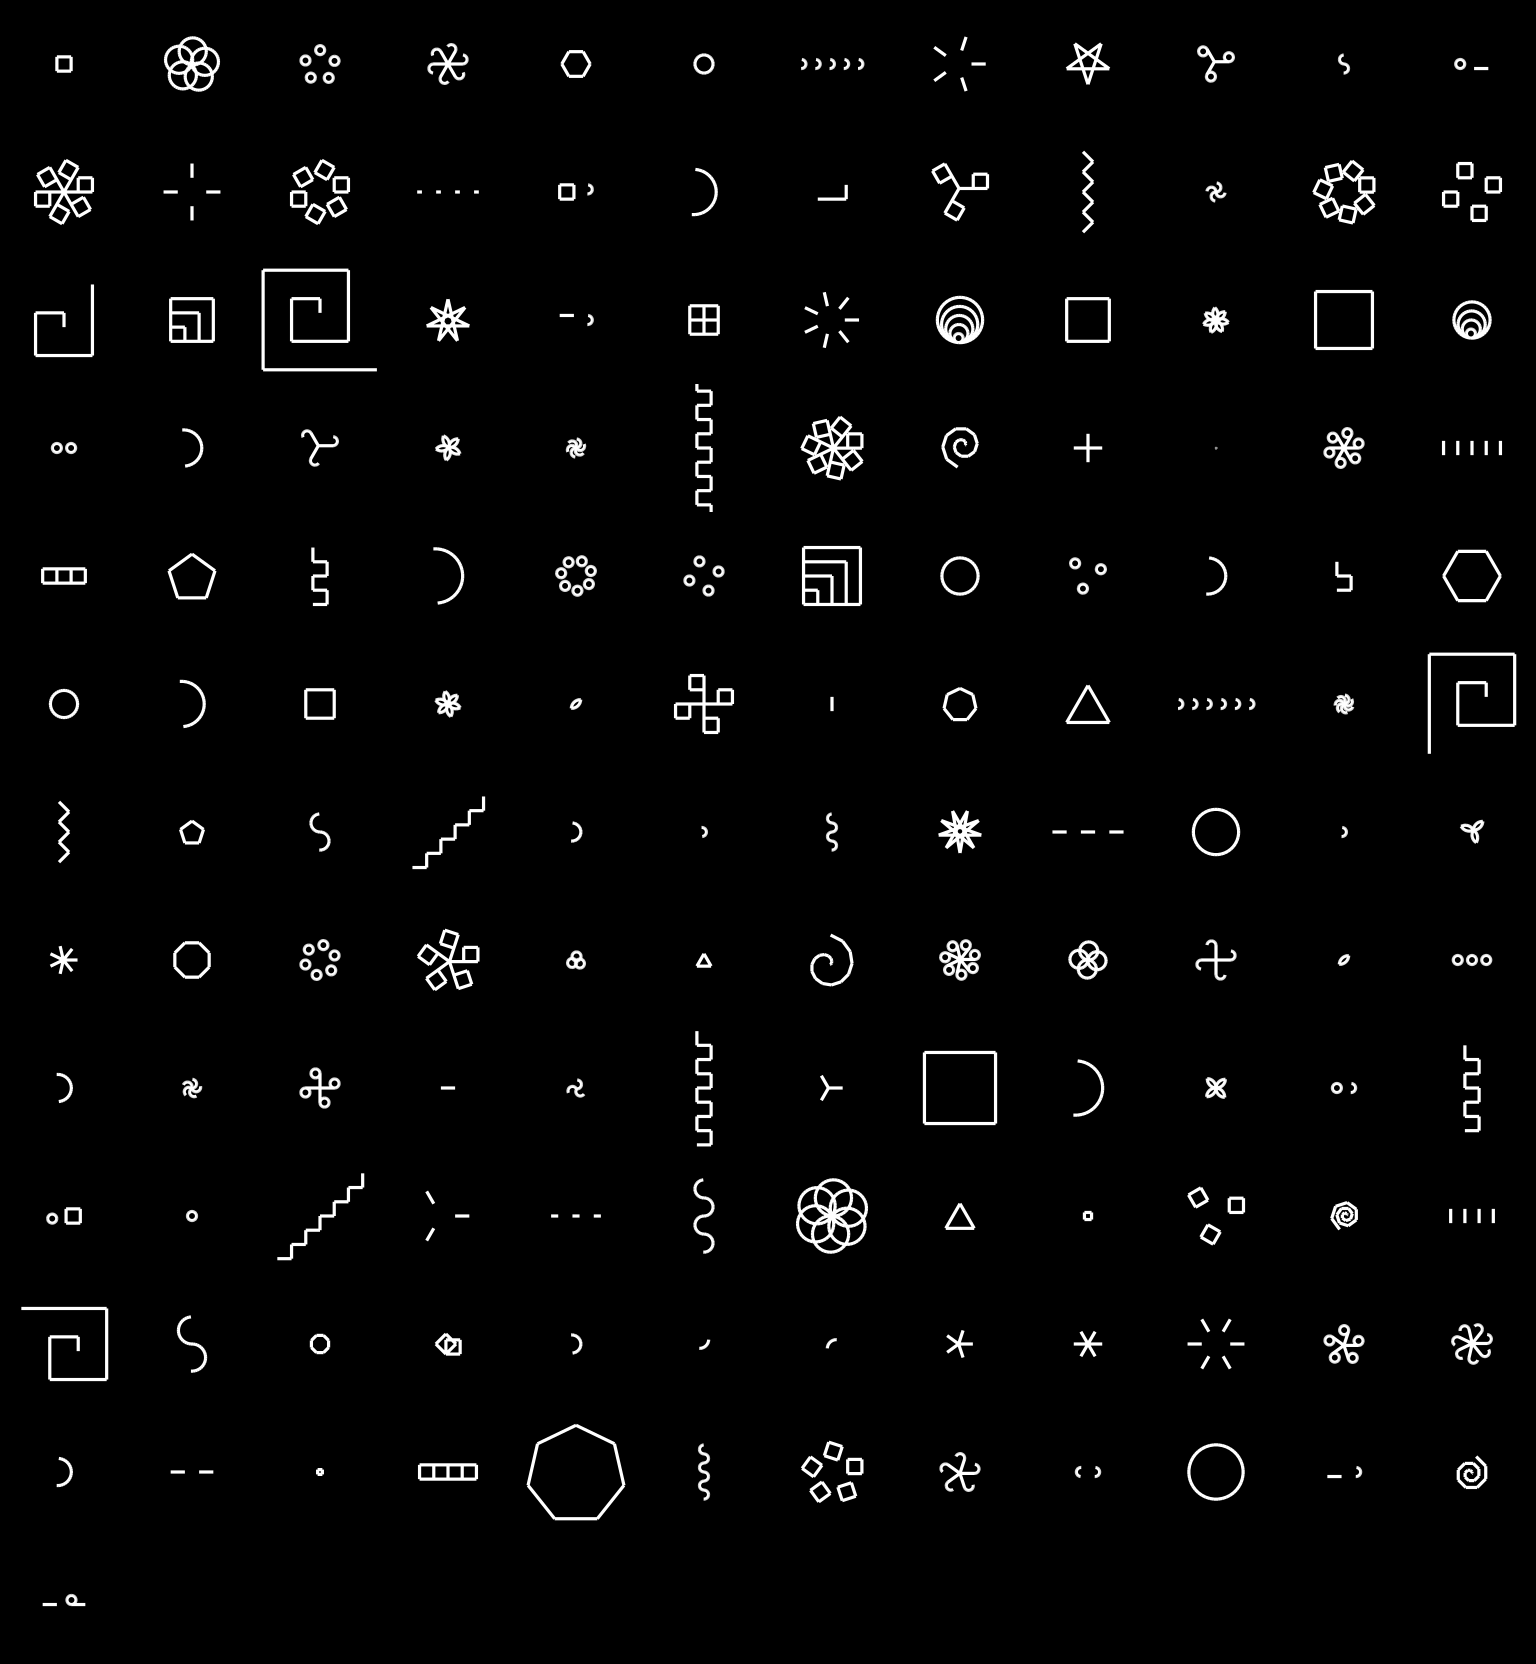
\includegraphics[width = \textwidth]{figures/fullLogo.png}
  \caption{Full set of LOGO graphics tasks that we apply our system to}
\end{figure}

\subsection{Full set of tower tasks}
\begin{figure}
  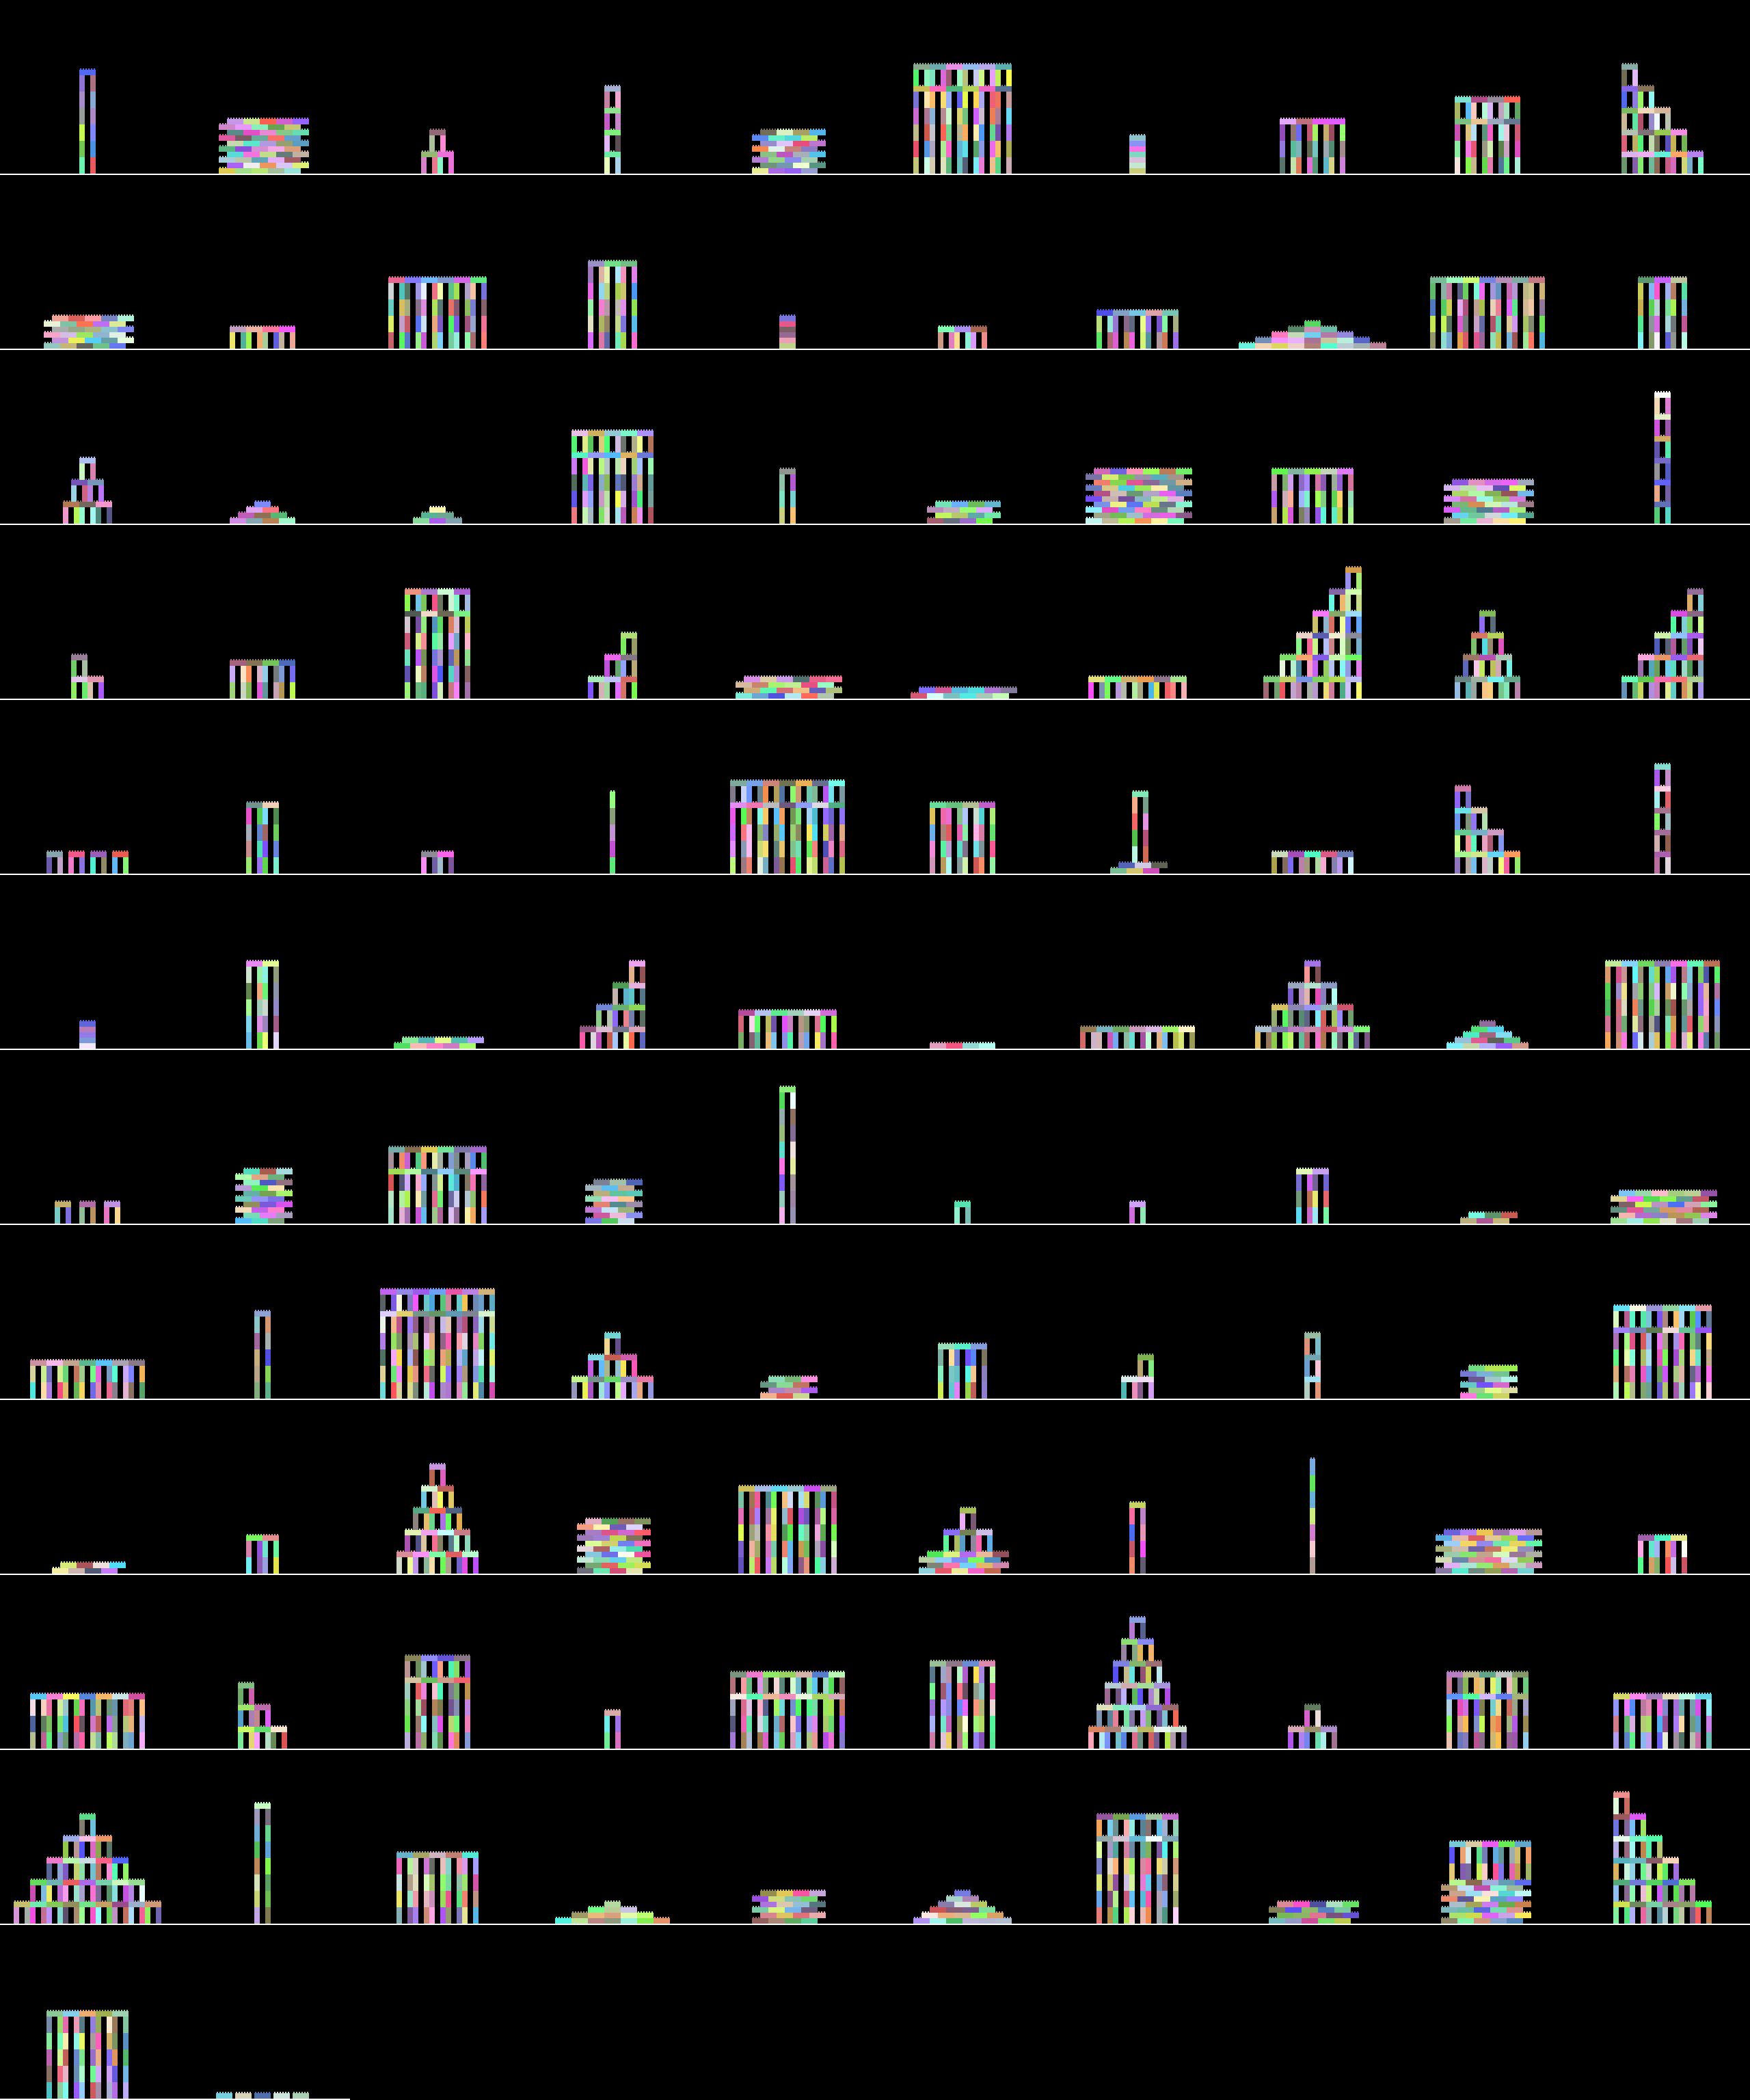
\includegraphics[width = \textwidth]{figures/fullTower.png}
  \caption{Full set of tower building tasks that we apply our system to}
\end{figure}

\subsection{Learning from Scratch: Tasks and DSL}\label{appendixMcCarthy}

We gave our system the following primitives: \code{if}, \code{=},
\code{>}, \code{+}, \code{-}, \code{0}, \code{1}, \code{cons},
\code{car}, \code{cdr}, \code{nil}, and \code{is-nil}, all of which
are present in some form in McCarthy's 1959
Lisp~\cite{mccarthy1960recursive}.\footnote{McCarthy's first version
  of Lisp used \code{cond} instead of \code{if}. Because we are using
  a typed language, we instead used \code{if}, because Lisp-style
  \code{cond} is unwieldy to express as a function in typed
  languages.}  We furthermore allowed functions to call themselves,
which we modeled using the Y combinator.  We did not use the
recognition model for this experiment: a bottom-up pattern recognizer
is of little use for acquiring this abstract knowledge from less than
two dozen problems.

Figure~\ref{learningFromScratch} shows the full set of tasks and the learned DSL.
\begin{figure*}  \newcommand{\helpSize}{0.25cm}
  \begin{tabular}{cc}\toprule
    \normalsize \pop{Programs} \& Tasks&\normalsize \popp{DSL}\\\midrule 
    
    \begin{tabular}{l}
      \code{[1\, 9]}$\to $\code{2}\\
      \code{[5\, 3\, 8]$\to$3}\\
    \blueCode{$f(\ell) = $($f_4$ $\ell$)}\\\\
      \code{[true\, false]}$\to $\code{2}\\
      \code{[false\, false\, false]$\to$3}\\
    \blueCode{$f(\ell) = $($f_4$ $\ell$)}\\\\

\code{[2\, 1\, 4]$\to$[2\, 1\, 4\, 0]}\\
%\code{[9\, 4\, 8]$\to$[9\, 4\, 8\, 0]}\\
\code{[9\, 8]$\to$[9\, 8\, 0]}\\
\blueCode{$f(\ell) = $($f_2$ cons $\ell$ (cons 0 nil))}\\\\

\code{[2\, 1\, 4]$\to$[2\, 1]}\\
%\code{[9\, 4\, 8]$\to$[9\, 4\, 8\, 0]}\\
\code{[9\, 8]$\to$[9]}\\
\blueCode{$f(\ell) = $($f_0$ ($\lambda$ (z) (empty? (cdr z))) car cdr $\ell$)}\\\\

\code{[2\, 5\, 6\, 0\, 6]$\to$19}\\
\code{[9\, 2\, 7\, 6\, 3]$\to$27}\\
\blueCode{$f(\ell) = $($f_2$ + $\ell$ 0)}\\\\

\code{[4\, 2\, 6\, 4]$\to$[8\, 4\, 12\, 8]}\\
%\code{[0\, 3\, 5\, 0\, 3\, 2]$\to$[0\, 6\, 10\, 0\, 6\, 4]}\\
\code{[2\, 3\, 0\, 7]$\to$[4\, 6\, 0\, 14]}\\
\blueCode{$f(\ell) = $($f_3$ ($\lambda$ (x) (+ x x)) $\ell$)}\\\\
\code{[4\, 2\, 6\, 4]$\to$[-4\, -2\, -6\, -4]}\\
%\code{[0\, 3\, 5\, 0\, 3\, 2]$\to$[0\, 6\, 10\, 0\, 6\, 4]}\\
\code{[2\, 3\, 0\, 7]$\to$[-2\, -3\, -0\, -7]}\\
\blueCode{$f(\ell) = $($f_3$ (- 0) $\ell$)}\\\\
\code{[4\, 2\, 6\, 4]$\to$[5\, 3\, 7\, 5]}\\
%\code{[0\, 3\, 5\, 0\, 3\, 2]$\to$[0\, 6\, 10\, 0\, 6\, 4]}\\
\code{[2\, 3\, 0\, 7]$\to$[3\, 4\, 1\, 8]}\\
\blueCode{$f(\ell) = $($f_3$ (+ 1) $\ell$)}\\\\



      \code{[1\, 5\, 2\, 9]}$\to$\code{[1\, 2]}\\
      \code{[3\, 8\, 1\, 3\, 1\, 2]}$\to$\code{[3\, 1\, 1]}\\
      \blueCode{$f(\ell) = $($f_0$ empty? car}\\
      \phantom{\blueCode{$f(\ell) = $($f_0$}}\blueCode{($\lambda$ (l) (cdr (cdr l))) $\ell$)}
      \\\\

      \code{3$\to $[0\, 1\, 2]}\\
      \code{2$\to $[0\, 1]}\\
      \blueCode{$f(n) = $($f_5$ ($\lambda$ (x) x) 0 $n$)}\\\\

      \code{3$\to $[0\, 1\, 2\, 3]}\\
      \code{2$\to $[0\, 1\, 2]}\\
      \blueCode{$f(n) = $($f_5$ ($\lambda$ (x) x) 0 (+ 1 $n$))}\\\\

      


      
      \end{tabular}&

%    \rotatebox[origin=c]{90}{\normalsize \popp{DSL}}&
    \begin{tabular}{l}
        \popp{\code{$f_0($p$,$f$,$n$,$x$)\,=\,$(if (p x) nil}}\\
      \phantom{\code{$f_1($f$,$l$,$x$)\,=\,$(if }}}\popp{\code{(cons (f x) ($f_0$ (n x))))}}\\
        \hspace{\helpSize}($f_0$: \emph{unfold})\\
        \popp{\code{$f_1($i$,$l$)\,=\,$(if (= i 0) (car l)}}\\
      \phantom{\code{$f_1($f$,$l$,$x$)\,=\,$(if}}}\popp{\code{($f_1$ (- i 1) (cdr l))))}}\\
        \hspace{\helpSize}($f_1$: \emph{index})\\
        \popp{\code{$f_2($f$,$l$,$x$)\,=\,$(if (empty? l) x}}\\
      \phantom{\code{$f_2($f$,$l$,$x$)\,=\,$(if }}}\popp{\code{(f (car l) ($f_2$ (cdr l))))}}\\
        \hspace{\helpSize}($f_2$: \emph{fold})\\
        \greenCode{$f_3($f$,$l$)\,=\,$($f_2$ nil l ($\lambda$ (x a) (cons (f x) a)))}\\
        \hspace{\helpSize}($f_3$: \emph{map})\\
        \greenCode{$f_4(\ell)$\,=\,(if (empty? $\ell$) 0 (+ 1 ($f_4$ (cdr $\ell$)))))}\\
        \hspace{\helpSize}($f_4$: \emph{length})\\
        \greenCode{$f_5(\code{f},\code{m},\code{n})$\,=\,($f_0$ (= m) f (+ 1) n)}\\
        \hspace{\helpSize}($f_5$: \emph{generalization of range})

%        -0.222777	int -> int -> list(int)	#(lambda (lambda (fix1 $0 (lambda (lambda (#(lambda (lambda (lambda (if $0 empty (cons $1 $2))))) (map (lambda (#(+ 1) $0)) ($1 (#(lambda (- $0 1)) $0))) 0 (eq? $0 $3)))))))

      \end{tabular}
    %% : (lambda (#(#(lambda (lambda (lambda (lambda (fix1 $0 (lambda (lambda (if (empty? $0) $3 ($4 ($5 $0) ($1 (cdr $0))))))))))) (lambda (car $0))) (lambda (lambda (+ $0 $1))) 0 $0))
    %% (lambda (lambda (lambda (lambda (fix1 $0 (lambda (lambda (#(lambda (lambda (lambda (if $0 empty (cons $1 $2))))) ($1 ($3 $0)) ($4 $0) ($5 $0)))))))))
    %% (lambda (lambda (fix1 $0 (lambda (lambda (#(lambda (lambda (lambda (if $0 empty (cons $1 $2))))) (#(lambda (lambda (fix1 $0 (lambda (lambda (if (empty? $0) empty (cons ($3 (car $0)) ($1 (cdr $0))))))))) (lambda (#(+ 1) $0)) ($1 (#(lambda (- $0 1)) $0))) 0 (eq? $0 $3)))))))
    \\\bottomrule 
    \end{tabular}
  \caption{Bootstrapping a standard library of functional programming routines, starting from recursion along with primitive operations found in 1959 Lisp.}\label{learningFromScratch}
  \end{figure*}


%% \begin{figure}
%%   \begin{tikzpicture}
%%     \node at (0,0) (d){DSL};
%%     \node at ([yshift = -2cm]d) (t){$\text{Task}$};

%%     \node at ([xshift = 2cm]t) (nn){
%%       \begin{tikzpicture}[x=2.5cm,y=1.25cm,transform canvas={scale=0.2,shift={+(-1,2.5)}}]
%%         \tikzstyle{neuron}=[circle,fill=blue!50,minimum size=20pt]
%%         \fill[fill=white] (-0.25,-0.5) rectangle (2.25,-4.5);
%%         \node[rectangle] at (1,1) {};
%%         \foreach \name / \y in {1,...,4}
%%             \node[neuron] (I-\name) at (0,-\y) {};
%%         \foreach \name / \y in {1,...,3}
%%             \node[neuron] (H-\name) at (1,-\y-0.5) {};
%%         \foreach \name / \y in {1,...,4}
%%             \node[neuron] (O-\name) at (2,-\y) {};
%%         \foreach \source in {1,...,4}
%%             \foreach \dest in {1,...,3}
%%                 \draw [-latex] (I-\source) -- (H-\dest);
%%         \foreach \source in {1,...,3}
%%             \foreach \dest in {1,...,4}
%%                 \draw [-latex] (H-\source) -- (O-\dest);
%%       \end{tikzpicture}
%%     };
%%     \node[align = center, text width = 1cm] at ([yshift = 0.6cm]nn.north) {\baselineskip=0pt \small Recognition model\par};
%%     \draw [->] (t.east) -- ([xshift = -0.5cm]nn.west);

%%     \node[draw,rounded corners, inner sep = 10] at ([xshift = 4.2cm,yshift = -1cm]) (s){Search};
%%     \node at ([xshift=-7pt,yshift=5pt]s.north west) {$\mathcal{D}$};

%%     \draw [->] ([xshift = 0.5cm]nn.east) -- ([yshift = -0.25cm]s.west);
%%     \draw [->,rounded corners] (d.east) -- ([yshift = 2cm]nn.center) -- ([yshift = 0.25cm]s.west);

%%     \node[align=left] at (7,-1) (f) {Frontier\\{\small (set of programs)}};
%%     \draw [->  ] (s.east) -- (f.west);

%%     \draw [->  ,rounded corners] (t.south) -- ([yshift = -0.5cm]t.south) -- ([yshift = -0.5cm] s.south |- t.south) -- (s.south);
%%     \node at ([xshift = 0.5cm,yshift = -0.75cm]s.south) {Spec};

%%     \node at (4,-3.5) {\textbf{\textsc{Wake: Problem Solving}}};
    
    
%%   \end{tikzpicture}

%%   \vspace{1cm}
  
  

%%   \begin{tikzpicture}
%%     \node at (0,0) (f1){Frontier$_1$};
%%     \node at ([yshift = -1cm]f1.south) (f2){Frontier$_2$};
%%     \node at ([yshift = -1cm]f2.south) (f3){Frontier$_3$};

%%     \node at ([xshift = 2cm]f1.east) (p1){program$_1$};
%%     \node at ([xshift = 2cm]f2.east) (p2){program$_2$};
%%     \node at ([xshift = 2cm]f3.east) (p3){program$_3$};


%%     \draw [->,squiggle ] (f1.east) -- node[above]{\small sample} (p1.west);
%%     \draw [->,squiggle ] (f2.east) -- node[above]{\small sample} (p2.west);
%%     \draw [->,squiggle ] (f3.east) -- node[above]{\small sample} (p3.west);
    
%%     \node at ([xshift = 1.5cm]p1.east) (t1){task$_1$};
%%     \node at ([xshift = 1.5cm]p2.east) (t2){task$_2$};
%%     \node at ([xshift = 1.5cm]p3.east) (t3){task$_3$};

%%     \node at ([yshift = -0.5cm]p3.south) {\textsc{\textbf{Sleep-R: Experience Replay}}};
%%   \end{tikzpicture}

%%   \begin{tikzpicture}
%%     \node[align=center] at (0,0) (d){DSL\\$(\mathcal{D},\theta)$};
%%     \node at ([xshift = 3cm]d.east) (p2){program};
%%     \node at ([yshift = 1.5cm]p2) (p1){program};
%%     \node at ([yshift = -1.5cm]p2) (p3){program};


%%     \draw[squiggle,-> ] (d.east) -- node[above]{\small sample} (p2.west);
%%     \draw[squiggle,-> ] (d.east) -- (p1.west);
%%     \draw[squiggle,-> ] (d.east) -- (p3.west);

%%     \node at ([xshift = 2cm]p1.east) (t1){task};
%%     \node at ([xshift = 2cm]p2.east) (t2){task};
%%     \node at ([xshift = 2cm]p3.east) (t3){task};
%%     \draw [-> ] (p1.east) -- node[above]{\small execute} (t1.west);
%%     \draw [-> ] (p3.east) -- node[above]{\small execute} (t3.west);
%%     \draw [-> ] (p2.east) -- node[above]{\small execute} (t2.west);

%%     \node at ([yshift = -0.5cm]p3.south) {\textsc{\textbf{Sleep-R: Dreaming}}};
%%   \end{tikzpicture}
  
%%   \vspace{2cm}
  
%%   \begin{tikzpicture}
%%     \node at (0,0) (f1){Frontier$_1$};
%%     \node at ([yshift = -1cm]f1.south) (f2){Frontier$_2$};
%%     \node at ([yshift = -0.7cm]f2.south) (ff){\textbf{$\vdots$}};
%%     \node at ([yshift = -1.2cm]f2.south) (ff){\textbf{$\vdots$}};
%%     \node at ([yshift = -1cm]ff.south) (f3){Frontier$_N$};

%%     \node(c)[rectangle, rounded corners, draw, minimum width = 3cm, minimum height = 6cm, anchor = north west] at (2,1) {};
%%     \node[anchor=north] at (c.north) {Compression};

%%     \draw [-> ] (f1.east) -- (c.west|-f1.east);
%%     \draw [-> ] (f2.east) -- (c.west|-f2.east);
%%     \draw [-> ] (f3.east) -- (c.west|-f3.east);

%%     \node[right](d) at ([xshift = 1.2cm,yshift = 0.7cm]c.east) {DSL $\mathcal{D}$};
%%     \node[right](t) at ([xshift = 1.2cm,yshift = -0.7cm]c.east) {Weights $\theta$};
%%     \draw [-> ] (c.east) -- (d.west);
%%     \draw [-> ] (c.east) -- (t.west);

%%     \node at (c.center) {
%% \begin{tikzpicture}[scale=0.7]
%%     %% \node[rotate=30] at (-2,0) {\begin{tabular}{c}
%%     %%     \footnotesize Program:\\
%%     %%     \code{($\lambda$ (x) (+ (- x) 1))}
%%     %% \end{tabular}};
%%     %\node at (,0.5) {\code{cons}};
%% %    \node [rotate=90] at (-2.3,-0.5) {\small program};
    
%%           \node(l1) at (0,0) {};
%%   \node[color=pop3](p1) at (-1,-1) {\code{+}};
%%   \node[color=pop3](n1) at (0.7,-0.9) {\code{1}};
%%   \node(x1) at (0,-1) {\code{1}};
%%   \draw[color=pop3] (l1.south) -- (p1.north);
%%   \draw[color=pop3] (l1.south) -- (n1.north);
%%   \draw[color=pop3] (-0.5,-0.45) -- (x1.north);

%%   \node(t) at (-0.5,0.5) {};
%%   \draw (l1.south) -- (t.south);
%%   \node(c) at (-1.5,-0.2) {\code{cons}};
%%   \draw (t.south) -- (c.north);
  
%% %    \draw  (l1.south) -- (-0.5,0.5);

%%   %% \node(c) at (-0.5,-1.5) {\code{-}};
%%   %% \node(z) at (0.5,-1.5) {\code{x}};

%%   %% \draw (0,-1) -- (c.north);
%%   %% \draw (0,-1) -- (z.north);
  
%%   \begin{scope}[shift={(-1,-2.5)}]
%%       \node(l1) at (0,0) {};
%%   \node[color=pop3](p1) at (-1,-1) {\code{+}};
%%   \node[color=pop3](n1) at (0.7,-0.9) {\code{1}};
%%   %\node(x1) at (0,-1) {};
%%   \draw[color=pop3] (l1.south) -- (p1.north);
%%   \draw[color=pop3] (l1.south) -- (n1.north);
%%   \draw[color=pop3] (-0.5,-0.45) -- (0,-1);


%%   \node(c) at (-0.5,-1.5) {\code{car}};
%%   \node(z) at (0.5,-1.5) {\code{z}};

%%   \draw (0,-1) -- (c.north);
%%   \draw (0,-1) -- (z.north);

%% %  \node [rotate=90] at (-2.3,-0.7) {\small program};
  
%%   \end{scope}

%% \begin{scope}[shift={(0,-5)}]
%%   \node[pop3](p1) at (-1,-1) {\code{+}};
%%   \node[pop3](n1) at (0.8,-0.7) {\code{1}};
%%   \node[pop3](a) at (0,-1) {\code{ }};
%%   %\node(x1) at (0,-1) {};
%%   \draw[pop3] (0,0) -- (p1.north);
%%   \draw[pop3] (0,0) -- (n1.north);
%%   \draw[pop3] (-0.55,-0.4) -- (a.north);
%% %  \node [rotate=90] at (-2.3,-0.7) {\small fragment};

%%   \end{scope}

%% \end{tikzpicture}
%%     };

%%     \node at ([yshift=-2.5cm,xshift = 4cm]c.south) {\textsc{\textbf{Sleep-G: Memory Consolidation}}};

%%     \end{tikzpicture}
%% \end{figure}

%% \begin{table*}%[t!]
%%   \makebox[\textwidth][c]{
%%     \scriptsize
%%   \tabcolsep=4pt
%%   \renewcommand\code\texttt
%%   \renewcommand\codechar[1]{\texttt{"#1"}}
%%   \newcommand{\helpSize}{0.25cm}
%%   \begin{tabular}{cccc}
%%     \toprule
%%     &{\normalsize Symbolic regression}&{\normalsize Laws of motion}&\\\midrule
%%     \rotatebox[origin=c]{90}{\normalsize \pop{Programs} \& Tasks}&{\tabcolsep=7pt
%%     \begin{tabular}{cc}
%%       
\includegraphics[width = 3em]{figures/functions/4.png}&
%%       
\includegraphics[width = 3em]{figures/functions/146}\\
%%       \pop{\code{$f($x$) = $($f_1$ x)}}&    \pop{\code{$f($x$) = $($f_6$ x)}}\\
%%       ~\\
%%       
\includegraphics[width = 3em]{figures/functions/112.png}&
%%         
\includegraphics[width = 3em]{figures/functions/92.png}
%%       \\
%%       \pop{\code{$f($x$) = $($f_4$ x)}}&    \pop{\code{$f($x$) = $($f_3$ x)}}\\

%%     \end{tabular}
%%     }
%%     &
%%     \begin{tabular}{cc}
%%       \includegraphics[width = 15em]{figures/massOnSpring.png} &
%%             \includegraphics[width = 15em]{figures/planets.png}
%%       \\
%%       \begin{tabular}{l}
%%               \blueCode{$f($o,$\Delta) = $($f_3$ o $\Delta$}\\
%%       \hspace{1cm}\blueCode{(- (* $k$ (pos o))}\\
%%       \hspace{1cm}\phantom{\code{(- }}\blueCode{(* $-9.8$ $\hat{x}$)))}\\
%%       \end{tabular}&
%%       \begin{tabular}{l}
%%               \blueCode{$f($a,b,$\Delta) = $($f_3$ a $\Delta$}\\
%%       \hspace{1cm}\blueCode{(/ (* $G$ (mass a) (mass b))}\\
%%       \hspace{1cm}\phantom{\code{(- }}\blueCode{(square (- (pos a) (pos b)))))}\\
%%         \end{tabular}
%%       \end{tabular}
%%     &

%%     ~\\
%%     \midrule
%%     \rotatebox[origin=c]{90}{\normalsize \popp{DSL}}&
%%       \begin{tabular}{l}
%%     \popp{$f_0($\code{x}$)\,=\,$\code{(+ x real)}}\\
%%     \popp{$f_1($\code{x}$)\,=\,$\code{($f_0$ (* real x))} }\\
%%     \popp{$f_2($\code{x}$)\,=\,$\code{($f_1$ (* x (}$f_0$\code{ x)))}}\\
%%     \popp{$f_3($\code{x}$)\,=\,$\code{($f_0$ (* x (}$f_2$\code{ x)))}}\\
%%     \popp{$f_4($\code{x}$)\,=\,$\code{($f_0$ (* x (}$f_3$\code{ x)))}}\\
%%     \hspace{\helpSize}\emph{($f_4$: 4th order polynomial)}\\
%%     \popp{$f_5($\code{x}$)\,=\,$\code{(/ real x)}}\\
%%     \popp{$f_6($\code{x}$)\,=\,$\code{($f_5$ ($f_0$ x))}}\\
%%     \hspace{\helpSize}\emph{($f_6$: rational function)}\\

%%   \end{tabular}
%%       &
%%       \begin{tabular}{l}
%%         \greenCode{$f_0($\code{o},$\Delta)\, = \,$(set-pos o (+ (pos o) (* $\Delta$ (vel o))))}\\
%%         \hspace{\helpSize}\emph{($f_0$: integrates position)}\\
%%         \greenCode{$f_1($\code{o},\code{a},$\Delta)\, = \,$(set-vel o (+ (vel o) (* $\Delta$ a)))}\\
%%         \hspace{\helpSize}\emph{($f_1$: integrates velocity)}\\
%%         \greenCode{$f_2($\code{o},\code{F}$)\, = \,$(/ F (mass o))}\\
%%         \hspace{\helpSize}\emph{($f_2$: Newton's second law)}\\
%%         \greenCode{$f_3($\code{o},$\Delta$,\code{F}$)\, = \,$($f_0$ o $\Delta$ ($f_1$ o ($f_2$ o F) $\Delta$))}\\
%%         \hspace{\helpSize}\emph{($f_3$: applies Newton's second law and integrates)}
        
%%         \end{tabular}


%% &


%%   \\\bottomrule\\
%% \end{tabular}}\vspace{-0.5cm} 
%% \caption{Top: Tasks from three domains we apply our algorithm to, each followed by the programs \system discovers for them. Bottom: Several examples from learned DSL. Notice that learned DSL primitives can call each other, and that \system rediscovers higher-order functions like \code{filter} ($f_1$ under List Functions)}\label{initialExampleDSL}%\vspace{-0.5cm}
%% \end{table*}


\end{document}
